\chapter{Defining computation}\label{compchap}

\begin{objectives} \label[objectives]{See-that-computation-can-}

\begin{itemize}
\tightlist
\item
  See that computation can be precisely modeled.\\
\item
  Learn the computational model of \emph{Boolean circuits} /
  \emph{straight-line programs}.
\item
  Equivalence of circuits and straight-line programs.
\item
  Equivalence of AND/OR/NOT and NAND.
\item
  Examples of computing in the physical world.\\
\end{itemize}

\end{objectives}

\begin{quote}
\emph{``there is no reason why mental as well as bodily labor should not
be economized by the aid of machinery''}, Charles Babbage, 1852
\end{quote}

\begin{quote}
\emph{``If, unwarned by my example, any man shall undertake and shall
succeed in constructing an engine embodying in itself the whole of the
executive department of mathematical analysis upon different principles
or by simpler mechanical means, I have no fear of leaving my reputation
in his charge, for he alone will be fully able to appreciate the nature
of my efforts and the value of their results.''}, Charles Babbage, 1864
\end{quote}

\begin{quote}
\emph{``To understand a program you must become both the machine and the
program.''}, Alan Perlis, 1982
\end{quote}


\begin{marginfigure}
\centering
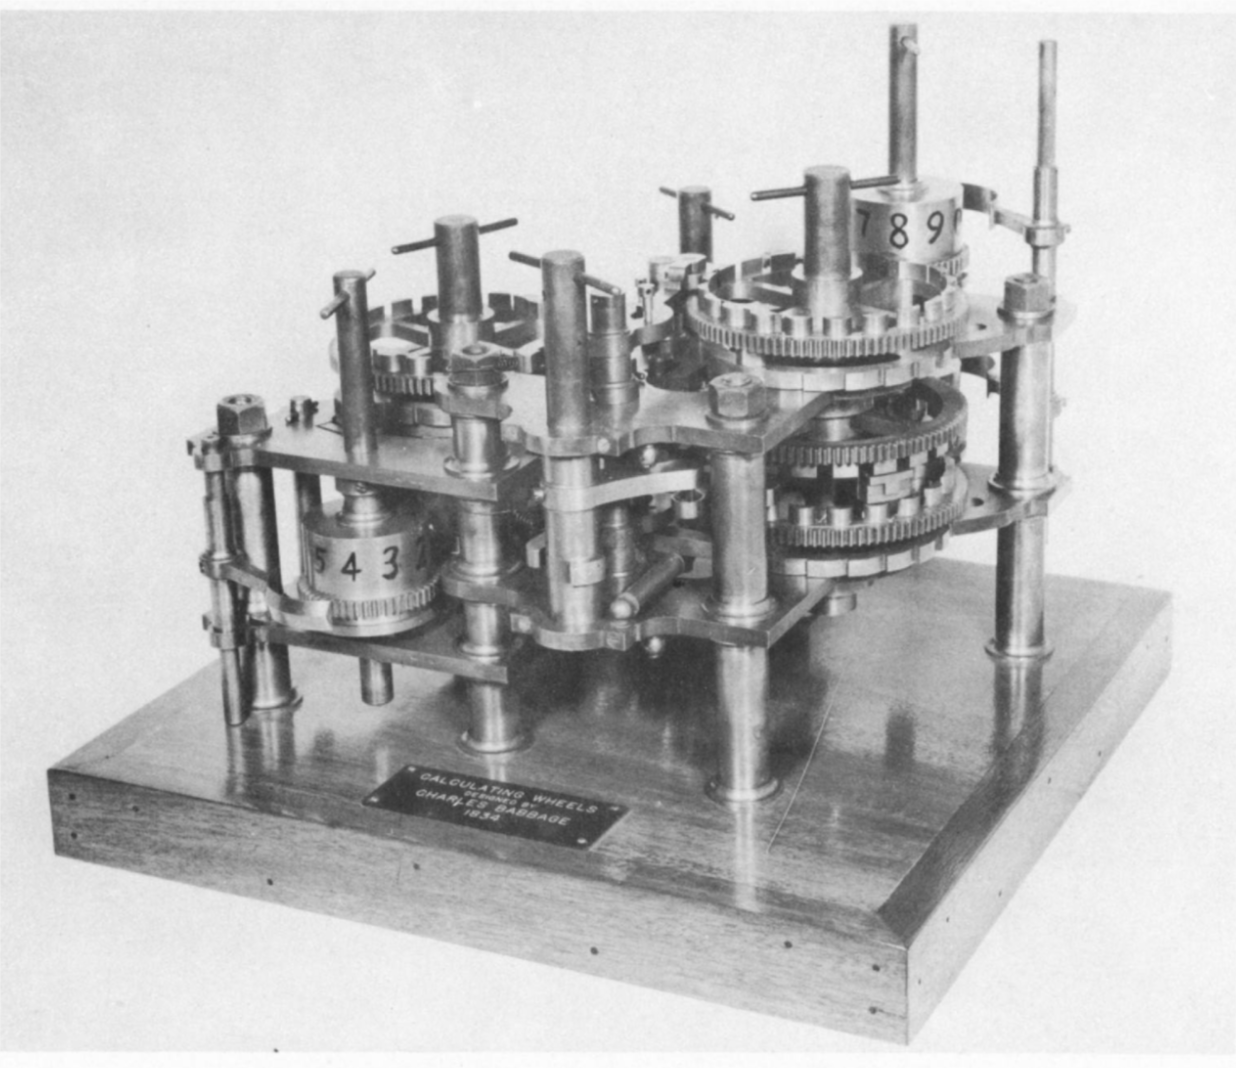
\includegraphics[width=\linewidth, height=1.5in, keepaspectratio]{../figure/wheels_babbage.png}
\caption{Calculating wheels by Charles Babbage. Image taken from the
Mark I `operating manual'}
\label{babbagewheels}
\end{marginfigure}


\begin{marginfigure}
\centering
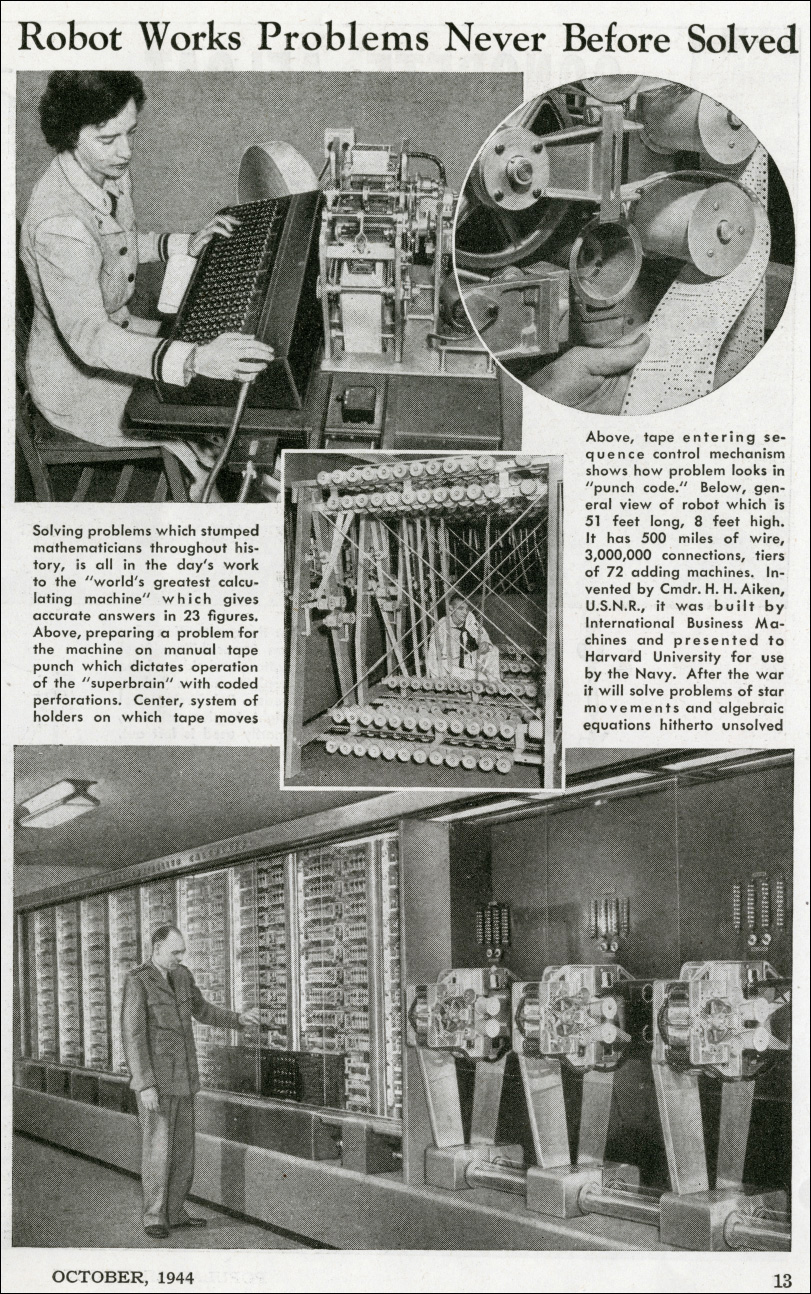
\includegraphics[width=\linewidth, height=1.5in, keepaspectratio]{../figure/PopularMechanics1944smaller.jpg}
\caption{A 1944 \emph{Popular Mechanics} article on the
\href{http://sites.harvard.edu/~chsi/markone/about.html}{Harvard Mark I
computer}.}
\label{markIcomp}
\end{marginfigure}

People have been computing for thousands of years, with aids that
include not just pen and paper, but also abacus, slide rules, various
mechanical devices, and modern electronic computers. A priori, the
notion of computation seems to be tied to the particular mechanism that
you use. You might think that the ``best'' algorithm for multiplying
numbers will differ if you implement it in \emph{Python} on a modern
laptop than if you use pen and paper. However, as we saw in the
introduction (\cref{chapintro}), an algorithm that is asymptotically
better would eventually beat a worse one regardless of the underlying
technology. This gives us hope for a \emph{technology independent} way
of defining computation. This is what we do in this chapter. We will
define the notion of computing an output from an input by applying a
sequence of basic operations (see \cref{compchapwhatvshowfig}). Using
this, we will be able to precisely define statements such as ``function
\(f\) can be computed by model \(X\)'' or ``function \(f\) can be
computed by model \(X\) using \(s\) operations''.


\begin{figure}
\centering
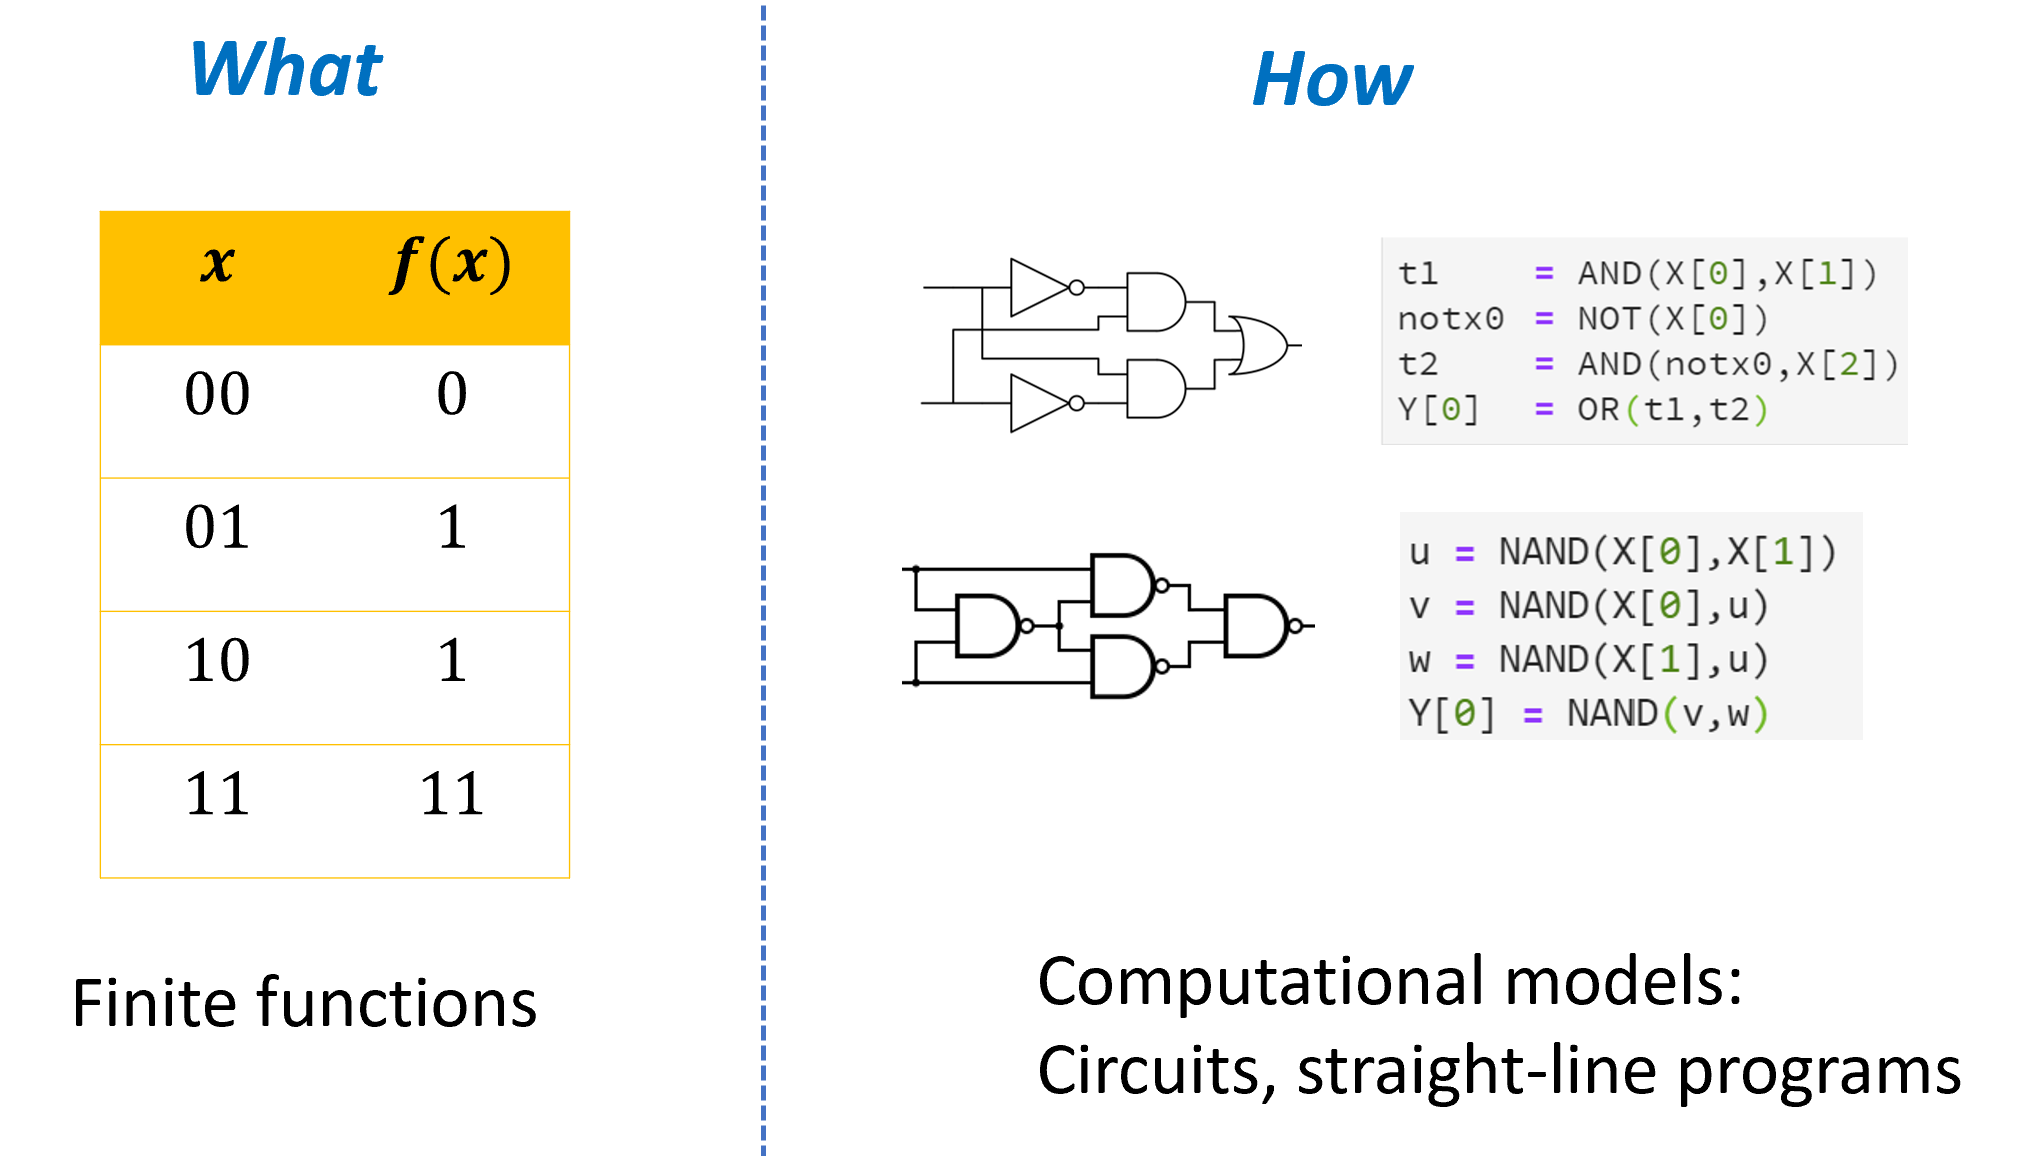
\includegraphics[width=\textwidth, height=0.25\paperheight, keepaspectratio]{../figure/compchapterwhatvshow.png}
\caption{A function mapping strings to strings \emph{specifies} a
computational task, i.e., describes \emph{what} the desired relation
between the input and the output is. In this chapter we define models
for \emph{implementing} computational processes that achieve the desired
relation, i.e., describe \emph{how} to compute the output from the
input. We will see several examples of such models using both Boolean
circuits and straight-line programming languages.}
\label{compchapwhatvshowfig}
\end{figure}

\section{Defining computation}\label{Defining-computation}

The name ``algorithm'' is derived from the Latin transliteration of
Muhammad ibn Musa al-Khwarizmi's name. Al-Khwarizmi was a Persian
scholar during the 9th century whose books introduced the western world
to the decimal positional numeral system, as well as to the solutions of
linear and quadratic equations (see \cref{alKhwarizmi}). However
Al-Khwarizmi's descriptions of algorithms were rather informal by
today's standards. Rather than use ``variables'' such as \(x,y\), he
used concrete numbers such as 10 and 39, and trusted the reader to be
able to extrapolate from these examples, much as algorithms are still
taught to children today.

Here is how Al-Khwarizmi described the algorithm for solving an equation
of the form \(x^2 +bx = c\):

\begin{quote}
\emph{{[}How to solve an equation of the form {]} ``roots and squares
are equal to numbers'': For instance ``one square , and ten roots of the
same, amount to thirty-nine dirhems'' that is to say, what must be the
square which, when increased by ten of its own root, amounts to
thirty-nine? The solution is this: you halve the number of the roots,
which in the present instance yields five. This you multiply by itself;
the product is twenty-five. Add this to thirty-nine' the sum is
sixty-four. Now take the root of this, which is eight, and subtract from
it half the number of roots, which is five; the remainder is three. This
is the root of the square which you sought for; the square itself is
nine.}
\end{quote}


\begin{marginfigure}
\centering
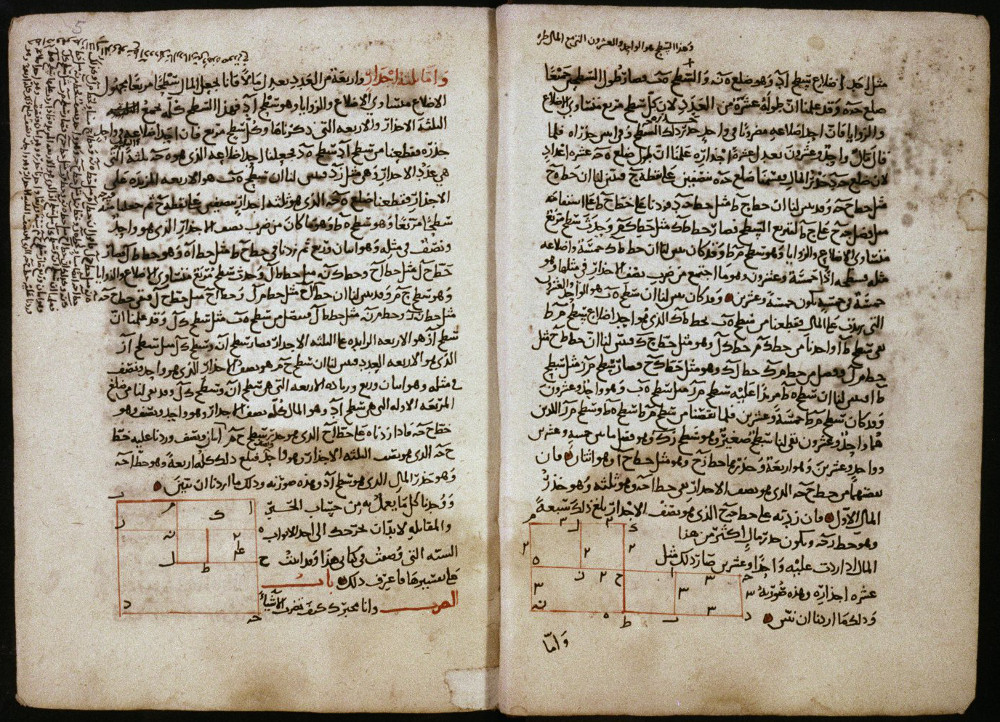
\includegraphics[width=\linewidth, height=1.5in, keepaspectratio]{../figure/alKhwarizmi.jpg}
\caption{Text pages from Algebra manuscript with geometrical solutions
to two quadratic equations. Shelfmark: MS. Huntington 214
fol.~004v-005r}
\label{alKhwarizmi}
\end{marginfigure}


\begin{marginfigure}
\centering
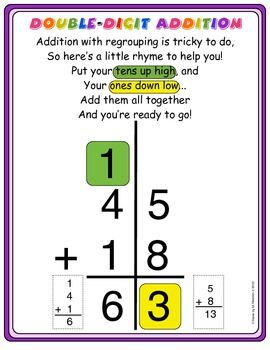
\includegraphics[width=\linewidth, height=1.5in, keepaspectratio]{../figure/addition_regrouping.jpg}
\caption{An explanation for children of the two digit addition
algorithm}
\label{childrenalg}
\end{marginfigure}

For the purposes of this book, we will need a much more precise way to
describe algorithms. Fortunately (or is it unfortunately?), at least at
the moment, computers lag far behind school-age children in learning
from examples. Hence in the 20th century, people came up with exact
formalisms for describing algorithms, namely \emph{programming
languages}. Here is al-Khwarizmi's quadratic equation solving algorithm
described in the \emph{Python} programming language:

\begin{code}
from math import sqrt
#Pythonspeak to enable use of the sqrt function to compute square roots.

def solve_eq(b,c):
    # return solution of x^2 + bx = c following Al Khwarizmi's instructions
    # Al Kwarizmi demonstrates this for the case b=10 and c= 39

    val1 = b / 2.0 # "halve the number of the roots"
    val2 = val1 * val1 # "this you multiply by itself"
    val3 = val2 + c # "Add this to thirty-nine"
    val4 = sqrt(val3) # "take the root of this"
    val5 = val4 - val1 # "subtract from it half the number of roots"
    return val5  # "This is the root of the square which you sought for"

# Test: solve x^2 + 10*x = 39
print(solve_eq(10,39))
# 3.0
\end{code}

We can define algorithms informally as follows:

\begin{quote} \label[quote]{Informal-definition-of-an}

\textbf{Informal definition of an algorithm:} An \emph{algorithm} is a
set of instructions for how to compute an output from an input by
following a sequence of ``elementary steps''.

An algorithm \(A\) \emph{computes} a function \(F\) if for every input
\(x\), if we follow the instructions of \(A\) on the input \(x\), we
obtain the output \(F(x)\).

\end{quote}

In this chapter we will make this informal definition precise using the
model of \textbf{Boolean Circuits}. We will show that Boolean Circuits
are equivalent in power to \textbf{straight line programs} that are
written in ``ultra simple'' programming languages that do not even have
loops. We will also see that the particular choice of \textbf{elementary
operations} is immaterial and many different choices yield models with
equivalent power (see \cref{compchapoverviewfig}). However, it will take
us some time to get there. We will start by discussing what are
``elementary operations'' and how we map a description of an algorithm
into an actual physical process that produces an output from an input in
the real world.


\begin{figure}
\centering
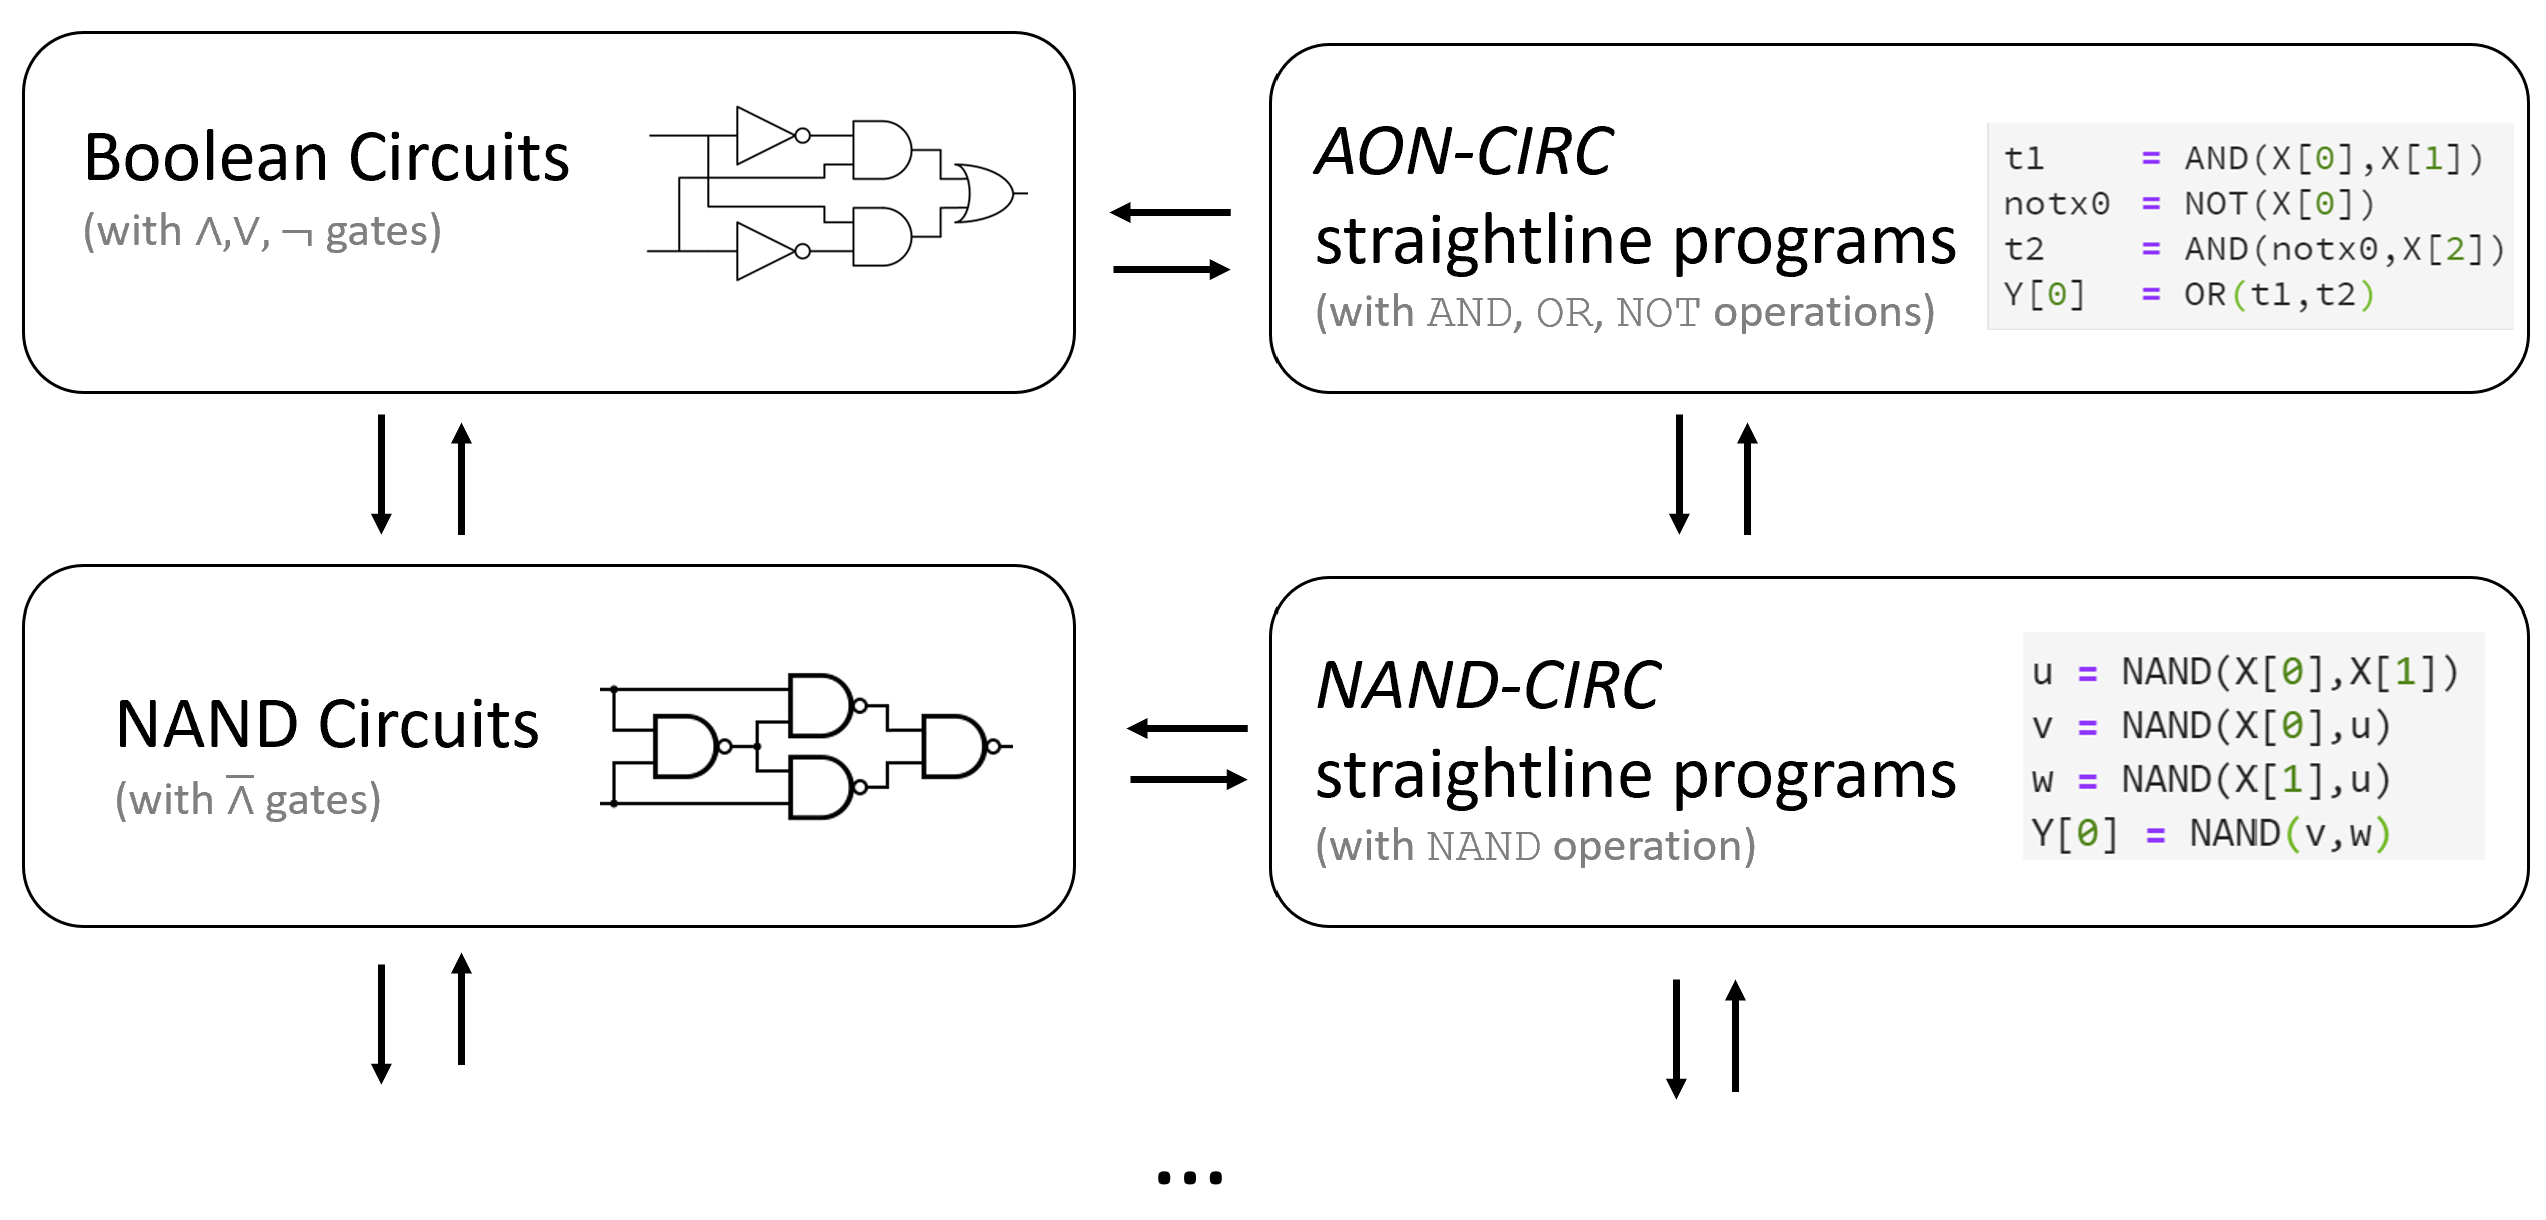
\includegraphics[width=\textwidth, height=0.25\paperheight, keepaspectratio]{../figure/compcharoverview.png}
\caption{An overview of the computational models defined in this
chapter. We will show several equivalent ways to represent a recipe for
performing a finite computation. Specifically we will show that we can
model such a computation using either a \emph{Boolean circuit} or a
\emph{straight line program}, and these two representations are
equivalent to one another. We will also show that we can choose as our
basic operations either the set
\(\{ \ensuremath{\mathit{AND}} , \ensuremath{\mathit{OR}} , \ensuremath{\mathit{NOT}} \}\)
or the set \(\{ \ensuremath{\mathit{NAND}} \}\) and these two choices
are equivalent in power. By making the choice of whether to use circuits
or programs, and whether to use
\(\{ \ensuremath{\mathit{AND}} , \ensuremath{\mathit{OR}} , \ensuremath{\mathit{NOT}} \}\)
or \(\{ \ensuremath{\mathit{NAND}} \}\) we obtain four equivalent ways
of modeling finite computation. Moreover, there are many other choices
of sets of basic operations that are equivalent in power.}
\label{compchapoverviewfig}
\end{figure}

\section{Computing using AND, OR, and
NOT.}\label{Computing-using-AND-OR-an}

An algorithm breaks down a \emph{complex} calculation into a series of
\emph{simpler} steps. These steps can be executed in a variety of
different ways, including:

\begin{itemize}
\item
  Writing down symbols on a piece of paper.
\item
  Modifying the current flowing on electrical wires.
\item
  Binding a protein to a strand of DNA.
\item
  Responding to a stimulus by a member of a collection (e.g., a bee in a
  colony, a trader in a market).
\end{itemize}

To formally define algorithms, let us try to ``err on the side of
simplicity'' and model our ``basic steps'' as truly minimal. For
example, here are some very simple functions:

\begin{itemize}
\tightlist
\item
  \(\ensuremath{\mathit{OR}}:\{0,1\}^2 \rightarrow \{0,1\}\) defined as
\end{itemize}

\[\ensuremath{\mathit{OR}}(a,b) = \begin{cases} 0 & a=b=0 \\ 1 & \text{otherwise} \end{cases}\]

\begin{itemize}
\tightlist
\item
  \(\ensuremath{\mathit{AND}}:\{0,1\}^2 \rightarrow \{0,1\}\) defined as
\end{itemize}

\[\ensuremath{\mathit{AND}}(a,b) = \begin{cases} 1 & a=b=1 \\ 0 & \text{otherwise} \end{cases}\]

\begin{itemize}
\tightlist
\item
  \(\ensuremath{\mathit{NOT}}:\{0,1\} \rightarrow \{0,1\}\) defined as
\end{itemize}

\[\ensuremath{\mathit{NOT}}(a) = \begin{cases} 0 & a = 1 \\ 1 & a = 0 \end{cases}\]

The functions \(\ensuremath{\mathit{AND}}\),
\(\ensuremath{\mathit{OR}}\) and \(\ensuremath{\mathit{NOT}}\), are the
basic logical operators used in logic and many computer systems. In the
context of logic, it is common to use the notation \(a \wedge b\) for
\(\ensuremath{\mathit{AND}}(a,b)\), \(a \vee b\) for
\(\ensuremath{\mathit{OR}}(a,b)\) and \(\overline{a}\) and \(\neg a\)
for \(\ensuremath{\mathit{NOT}}(a)\), and we will use this notation as
well.

Each one of the functions
\(\ensuremath{\mathit{AND}},\ensuremath{\mathit{OR}},\ensuremath{\mathit{NOT}}\)
takes either one or two single bits as input, and produces a single bit
as output. Clearly, it cannot get much more basic than that. However,
the power of computation comes from \emph{composing} such simple
building blocks together.

\hypertarget{majorityfunctionex}{}
\begin{example}[Majority from $AND$,$OR$ and $NOT$] \label[example]{majorityfunctionex}

Consider the function
\(\ensuremath{\mathit{MAJ}}:\{0,1\}^3 \rightarrow \{0,1\}\) that is
defined as follows:

\[\ensuremath{\mathit{MAJ}}(x) = \begin{cases}1 & x_0 + x_1 + x_2 \geq 2 \\ 0 & \text{otherwise}\end{cases} \;.\]

That is, for every \(x\in \{0,1\}^3\),
\(\ensuremath{\mathit{MAJ}}(x)=1\) if and only if the majority (i.e., at
least two out of the three) of \(x\)'s elements are equal to \(1\). Can
you come up with a formula involving \(\ensuremath{\mathit{AND}}\),
\(\ensuremath{\mathit{OR}}\) and \(\ensuremath{\mathit{NOT}}\) to
compute \(\ensuremath{\mathit{MAJ}}\)? (It would be useful for you to
pause at this point and work out the formula for yourself. As a hint,
although the \(\ensuremath{\mathit{NOT}}\) operator is needed to compute
some functions, you will not need to use it to compute
\(\ensuremath{\mathit{MAJ}}\).)

Let us first try to rephrase \(\ensuremath{\mathit{MAJ}}(x)\) in words:
``\(\ensuremath{\mathit{MAJ}}(x)=1\) if and only if there exists some
pair of distinct elements \(i,j\) such that both \(x_i\) and \(x_j\) are
equal to \(1\).'' In other words it means that
\(\ensuremath{\mathit{MAJ}}(x)=1\) iff \emph{either} both \(x_0=1\)
\emph{and} \(x_1=1\), \emph{or} both \(x_1=1\) \emph{and} \(x_2=1\),
\emph{or} both \(x_0=1\) \emph{and} \(x_2=1\). Since the
\(\ensuremath{\mathit{OR}}\) of three conditions \(c_0,c_1,c_2\) can be
written as
\(\ensuremath{\mathit{OR}}(c_0,\ensuremath{\mathit{OR}}(c_1,c_2))\), we
can now translate this into a formula as follows:

\[
\ensuremath{\mathit{MAJ}}(x_0,x_1,x_2) = \ensuremath{\mathit{OR}}\left(\, \ensuremath{\mathit{AND}}(x_0,x_1)\;,\; \ensuremath{\mathit{OR}} \bigl( \ensuremath{\mathit{AND}}(x_1,x_2) \;,\; \ensuremath{\mathit{AND}}(x_0,x_2) \bigr) \, \right) \;. \label{eqmajandornot}
\]

Recall that we can also write \(a \vee b\) for
\(\ensuremath{\mathit{OR}}(a,b)\) and \(a \wedge b\) for
\(\ensuremath{\mathit{AND}}(a,b)\). With this notation,
\eqref{eqmajandornot} can also be written as

\[\ensuremath{\mathit{MAJ}}(x_0,x_1,x_2) = ((x_0 \wedge x_1) \vee (x_1 \wedge x_2)) \vee (x_0 \wedge x_2)\;.\]

We can also write \eqref{eqmajandornot} in a ``programming language''
format, expressing it as a set of instructions for computing
\(\ensuremath{\mathit{MAJ}}\) given the basic operations
\(\ensuremath{\mathit{AND}},\ensuremath{\mathit{OR}},\ensuremath{\mathit{NOT}}\):

\begin{code}
def MAJ(X[0],X[1],X[2]):
    firstpair  = AND(X[0],X[1])
    secondpair = AND(X[1],X[2])
    thirdpair  = AND(X[0],X[2])
    temp       = OR(secondpair,thirdpair)
    return OR(firstpair,temp)
\end{code}

\end{example}

\subsection{Some properties of AND and
OR}\label{Some-properties-of-AND-an}

Like standard addition and multiplication, the functions
\(\ensuremath{\mathit{AND}}\) and \(\ensuremath{\mathit{OR}}\) satisfy
the properties of \emph{commutativity}: \(a \vee b = b \vee a\) and
\(a \wedge b = b \wedge a\) and \emph{associativity}:
\((a \vee b) \vee c = a \vee (b \vee c)\) and
\((a \wedge b) \wedge c = a \wedge (b \wedge c)\). As in the case of
addition and multiplication, we often drop the parenthesis and write
\(a \vee b \vee c \vee d\) for \(((a \vee b) \vee c) \vee d\), and
similarly OR's and AND's of more terms. They also satisfy a variant of
the distributive law:

\hypertarget{distributivelaw}{}
\begin{solvedexercise}[Distributive law for AND and OR] \label[solvedexercise]{distributivelaw}

Prove that for every \(a,b,c \in \{0,1\}\),
\(a \wedge (b \vee c) = (a \wedge b) \vee (a \wedge c)\).

\end{solvedexercise}

\begin{solution} \label[solution]{We-can-prove-this-by-enum}

We can prove this by enumerating over all the \(8\) possible values for
\(a,b,c \in \{0,1\}\) but it also follows from the standard distributive
law. Suppose that we identify any positive integer with ``true'' and the
value zero with ``false''. Then for every numbers \(u,v \in \N\),
\(u+v\) is positive if and only if \(u \vee v\) is true and
\(u \cdot v\) is positive if and only if \(u \wedge v\) is true. This
means that for every \(a,b,c \in \{0,1\}\), the expression
\(a \wedge (b \vee c)\) is true if and only if \(a \cdot(b+c)\) is
positive, and the expression \((a \wedge b) \vee (a \wedge c)\) is true
if and only if \(a \cdot b + a \cdot c\) is positive, But by the
standard distributive law \(a\cdot (b+c) = a\cdot b + a \cdot c\) and
hence the former expression is true if and only if the latter one is.

\end{solution}

\subsection{Extended example: Computing \(\ensuremath{\mathit{XOR}}\)
from \(\ensuremath{\mathit{AND}}\), \(\ensuremath{\mathit{OR}}\), and
\(\ensuremath{\mathit{NOT}}\)}\label{xoraonexample}

Let us see how we can obtain a different function from the same building
blocks. Define
\(\ensuremath{\mathit{XOR}}:\{0,1\}^2 \rightarrow \{0,1\}\) to be the
function \(\ensuremath{\mathit{XOR}}(a,b)= a + b \mod 2\). That is,
\(\ensuremath{\mathit{XOR}}(0,0)=\ensuremath{\mathit{XOR}}(1,1)=0\) and
\(\ensuremath{\mathit{XOR}}(1,0)=\ensuremath{\mathit{XOR}}(0,1)=1\). We
claim that we can construct \(\ensuremath{\mathit{XOR}}\) using only
\(\ensuremath{\mathit{AND}}\), \(\ensuremath{\mathit{OR}}\), and
\(\ensuremath{\mathit{NOT}}\).

\begin{pause} \label[pause]{As-usual-it-is-a-good-exe}

As usual, it is a good exercise to try to work out the algorithm for
\(\ensuremath{\mathit{XOR}}\) using \(\ensuremath{\mathit{AND}}\),
\(\ensuremath{\mathit{OR}}\) and \(\ensuremath{\mathit{NOT}}\) on your
own before reading further.

\end{pause}

The following algorithm computes \(\ensuremath{\mathit{XOR}}\) using
\(\ensuremath{\mathit{AND}}\), \(\ensuremath{\mathit{OR}}\), and
\(\ensuremath{\mathit{NOT}}\):

\begin{algorithm}[$XOR$ from $AND$/$OR$/$NOT$]
\label[algorithm]{XORfromAONalg} ~ \\ \noindent
\begin{algorithmic}[1]
\INPUT  $a,b \in \{0,1\}$.
\OUTPUT  $XOR(a,b)$
\STATE $w1 \leftarrow AND(a,b)$
\STATE $w2 \leftarrow NOT(w1)$
\STATE $w3 \leftarrow OR(a,b)$
\RETURN $AND(w2,w3)$
\end{algorithmic}
\end{algorithm}

\hypertarget{alganalaysis}{}
\begin{lemma} \label[lemma]{alganalaysis}

For every \(a,b\in \{0,1\}\), on input \(a,b\), \cref{XORfromAONalg}
outputs \(a+b \mod 2\).

\end{lemma}

\begin{proof} \label[proof]{For-every-ab-ensuremathma}

For every \(a,b\), \(\ensuremath{\mathit{XOR}}(a,b)=1\) if and only if
\(a\) is \emph{different} from \(b\). On input \(a,b\in \{0,1\}\),
\cref{XORfromAONalg} outputs \(\ensuremath{\mathit{AND}}(w2,w3)\) where
\(w2=\ensuremath{\mathit{NOT}}(\ensuremath{\mathit{AND}}(a,b))\) and
\(w3=\ensuremath{\mathit{OR}}(a,b)\).

\begin{itemize}
\item
  If \(a=b=0\) then \(w3=\ensuremath{\mathit{OR}}(a,b)=0\) and so the
  output will be \(0\).
\item
  If \(a=b=1\) then \(\ensuremath{\mathit{AND}}(a,b)=1\) and so
  \(w2=\ensuremath{\mathit{NOT}}(\ensuremath{\mathit{AND}}(a,b))=0\) and
  the output will be \(0\).
\item
  If \(a=1\) and \(b=0\) (or vice versa) then both
  \(w3=\ensuremath{\mathit{OR}}(a,b)=1\) and
  \(w1=\ensuremath{\mathit{AND}}(a,b)=0\), in which case the algorithm
  will output
  \(\ensuremath{\mathit{OR}}(\ensuremath{\mathit{NOT}}(w1),w3)=1\).
\end{itemize}

\end{proof}

We can also express \cref{XORfromAONalg} using a programming language.
Specifically, the following is a \emph{Python} program that computes the
\(\ensuremath{\mathit{XOR}}\) function:

\begin{code}
def AND(a,b): return a*b
def OR(a,b):  return 1-(1-a)*(1-b)
def NOT(a):   return 1-a

def XOR(a,b):
    w1 = AND(a,b)
    w2 = NOT(w1)
    w3 = OR(a,b)
    return AND(w2,w3)

# Test out the code
print([f"XOR({a},{b})={XOR(a,b)}" for a in [0,1] for b in [0,1]])
# ['XOR(0,0)=0', 'XOR(0,1)=1', 'XOR(1,0)=1', 'XOR(1,1)=0']
\end{code}

\hypertarget{xorthreebits}{}
\begin{solvedexercise}[Compute $XOR$ on three bits of input] \label[solvedexercise]{xorthreebits}

Let \(\ensuremath{\mathit{XOR}}_3:\{0,1\}^3 \rightarrow \{0,1\}\) be the
function defined as
\(\ensuremath{\mathit{XOR}}_3(a,b,c) = a + b +c \mod 2\). That is,
\(\ensuremath{\mathit{XOR}}_3(a,b,c)=1\) if \(a+b+c\) is odd, and
\(\ensuremath{\mathit{XOR}}_3(a,b,c)=0\) otherwise. Show that you can
compute \(\ensuremath{\mathit{XOR}}_3\) using AND, OR, and NOT. You can
express it as a formula, use a programming language such as Python, or
use a Boolean circuit.

\end{solvedexercise}

\begin{solution} \label[solution]{Addition-modulo-two-satis}

Addition modulo two satisfies the same properties of
\emph{associativity} (\((a+b)+c=a+(b+c)\)) and \emph{commutativity}
(\(a+b=b+a\)) as standard addition. This means that, if we define
\(a \oplus b\) to equal \(a + b \mod 2\), then \[
\ensuremath{\mathit{XOR}}_3(a,b,c) = (a \oplus b) \oplus c
\] or in other words \[
\ensuremath{\mathit{XOR}}_3(a,b,c) = \ensuremath{\mathit{XOR}}(\ensuremath{\mathit{XOR}}(a,b),c) \;.
\]

Since we know how to compute \(\ensuremath{\mathit{XOR}}\) using AND,
OR, and NOT, we can compose this to compute
\(\ensuremath{\mathit{XOR}}_3\) using the same building blocks. In
Python this corresponds to the following program:

\begin{code}
def XOR3(a,b,c):
    w1 = AND(a,b)
    w2 = NOT(w1)
    w3 = OR(a,b)
    w4 = AND(w2,w3)
    w5 = AND(w4,c)
    w6 = NOT(w5)
    w7 = OR(w4,c)
    return AND(w6,w7)

# Let's test this out
print([f"XOR3({a},{b},{c})={XOR3(a,b,c)}" for a in [0,1] for b in [0,1] for c in [0,1]])
# ['XOR3(0,0,0)=0', 'XOR3(0,0,1)=1', 'XOR3(0,1,0)=1', 'XOR3(0,1,1)=0', 'XOR3(1,0,0)=1', 'XOR3(1,0,1)=0', 'XOR3(1,1,0)=0', 'XOR3(1,1,1)=1']
\end{code}

\end{solution}

\begin{pause} \label[pause]{Try-to-generalize-the-abo}

Try to generalize the above examples to obtain a way to compute
\(\ensuremath{\mathit{XOR}}_n:\{0,1\}^n \rightarrow \{0,1\}\) for every
\(n\) using at most \(4n\) basic steps involving applications of a
function in
\(\{ \ensuremath{\mathit{AND}}, \ensuremath{\mathit{OR}} , \ensuremath{\mathit{NOT}} \}\)
to outputs or previously computed values.

\end{pause}

\subsection{Informally defining ``basic operations'' and
``algorithms''}\label{Informally-defining-basic}

We have seen that we can obtain at least some examples of interesting
functions by composing together applications of
\(\ensuremath{\mathit{AND}}\), \(\ensuremath{\mathit{OR}}\), and
\(\ensuremath{\mathit{NOT}}\). This suggests that we can use
\(\ensuremath{\mathit{AND}}\), \(\ensuremath{\mathit{OR}}\), and
\(\ensuremath{\mathit{NOT}}\) as our ``basic operations'', hence
obtaining the following definition of an ``algorithm'':

\begin{quote} \label[quote]{Semi-formal-definition-of}

\textbf{Semi-formal definition of an algorithm:} An \emph{algorithm}
consists of a sequence of steps of the form ``compute a new value by
applying \(\ensuremath{\mathit{AND}}\), \(\ensuremath{\mathit{OR}}\), or
\(\ensuremath{\mathit{NOT}}\) to previously computed values''.

An algorithm \(A\) \emph{computes} a function \(F\) if for every input
\(x\) to \(F\), if we feed \(x\) as input to the algorithm, the value
computed in its last step is \(F(x)\).

\end{quote}

There are several concerns that are raised by this definition:

\begin{enumerate}
\def\labelenumi{\arabic{enumi}.}
\item
  First and foremost, this definition is indeed too informal. We do not
  specify exactly what each step does, nor what it means to ``feed \(x\)
  as input''.
\item
  Second, the choice of \(\ensuremath{\mathit{AND}}\),
  \(\ensuremath{\mathit{OR}}\) or \(\ensuremath{\mathit{NOT}}\) seems
  rather arbitrary. Why not \(\ensuremath{\mathit{XOR}}\) and
  \(\ensuremath{\mathit{MAJ}}\)? Why not allow operations like addition
  and multiplication? What about any other logical constructions such
  \texttt{if}/\texttt{then} or \texttt{while}?
\item
  Third, do we even know that this definition has anything to do with
  actual computing? If someone gave us a description of such an
  algorithm, could we use it to actually compute the function in the
  real world?
\end{enumerate}

\begin{pause} \label[pause]{These-concerns-will-to-a-}

These concerns will to a large extent guide us in the upcoming chapters.
Thus you would be well advised to re-read the above informal definition
and see what you think about these issues.

\end{pause}

A large part of this book will be devoted to addressing the above
issues. We will see that:

\begin{enumerate}
\def\labelenumi{\arabic{enumi}.}
\item
  We can make the definition of an algorithm fully formal, and so give a
  precise mathematical meaning to statements such as ``Algorithm \(A\)
  computes function \(f\)''.
\item
  While the choice of
  \(\ensuremath{\mathit{AND}}\)/\(\ensuremath{\mathit{OR}}\)/\(\ensuremath{\mathit{NOT}}\)
  is arbitrary, and we could just as well have chosen other functions,
  we will also see this choice does not matter much. We will see that we
  would obtain the same computational power if we instead used addition
  and multiplication, and essentially every other operation that could
  be reasonably thought of as a basic step.
\item
  It turns out that we can and do compute such
  ``\(\ensuremath{\mathit{AND}}\)/\(\ensuremath{\mathit{OR}}\)/\(\ensuremath{\mathit{NOT}}\)
  based algorithms'' in the real world. First of all, such an algorithm
  is clearly well specified, and so can be executed by a human with a
  pen and paper. Second, there are a variety of ways to \emph{mechanize}
  this computation. We've already seen that we can write Python code
  that corresponds to following such a list of instructions. But in fact
  we can directly implement operations such as
  \(\ensuremath{\mathit{AND}}\), \(\ensuremath{\mathit{OR}}\), and
  \(\ensuremath{\mathit{NOT}}\) via electronic signals using components
  known as \emph{transistors}. This is how modern electronic computers
  operate.
\end{enumerate}

In the remainder of this chapter, and the rest of this book, we will
begin to answer some of these questions. We will see more examples of
the power of simple operations to compute more complex operations
including addition, multiplication, sorting and more. We will also
discuss how to \emph{physically implement} simple operations such as
\(\ensuremath{\mathit{AND}}\), \(\ensuremath{\mathit{OR}}\) and
\(\ensuremath{\mathit{NOT}}\) using a variety of technologies.

\section{Boolean Circuits}\label{booleancircuitfig}


\begin{marginfigure}
\centering
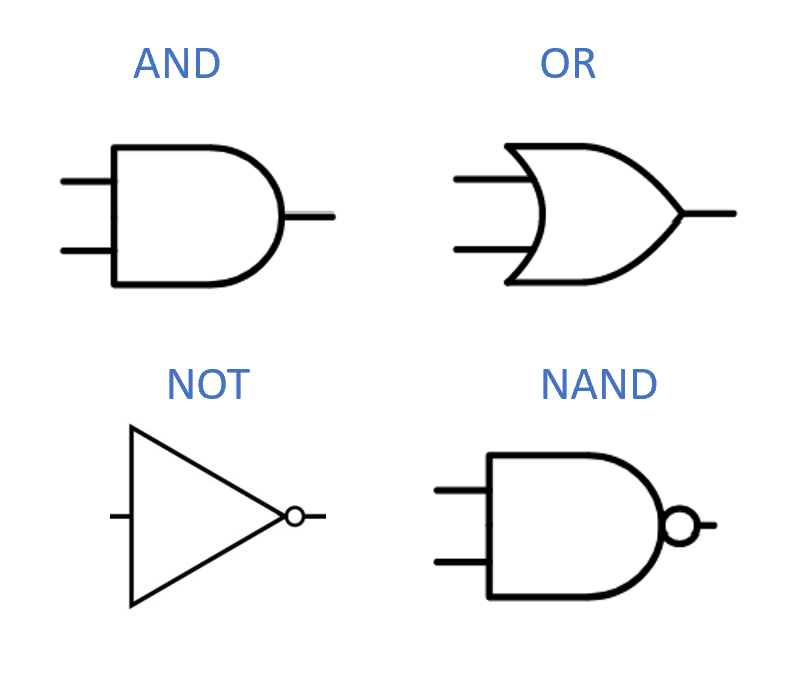
\includegraphics[width=\linewidth, height=1.5in, keepaspectratio]{../figure/logicgates.png}
\caption{Standard symbols for the logical operations or ``gates'' of
\(\ensuremath{\mathit{AND}}\), \(\ensuremath{\mathit{OR}}\),
\(\ensuremath{\mathit{NOT}}\), as well as the operation
\(\ensuremath{\mathit{NAND}}\) discussed in \cref{nandsec}.}
\label{logicgatesfig}
\end{marginfigure}


\begin{marginfigure}
\centering
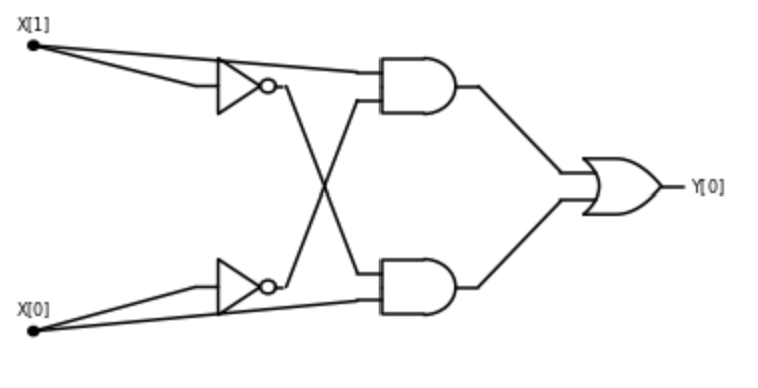
\includegraphics[width=\linewidth, height=1.5in, keepaspectratio]{../figure/xorcircuitschemdraw.png}
\caption{A circuit with \(\ensuremath{\mathit{AND}}\),
\(\ensuremath{\mathit{OR}}\) and \(\ensuremath{\mathit{NOT}}\) gates for
computing the \(\ensuremath{\mathit{XOR}}\) function.}
\label{andornotcircxorfig}
\end{marginfigure}

\emph{Boolean circuits} provide a precise notion of ``composing basic
operations together''. A Boolean circuit (see \cref{boolancircfig}) is
composed of \emph{gates} and \emph{inputs} that are connected by
\emph{wires}. The \emph{wires} carry a signal that represents either the
value \(0\) or \(1\). Each gate corresponds to either the \emph{OR},
\emph{AND}, or \emph{NOT} operation. An \emph{OR gate} has two incoming
wires, and one or more outgoing wires. If these two incoming wires carry
the signals \(a\) and \(b\) (for \(a,b \in \{0,1\}\)), then the signal
on the outgoing wires will be \(\ensuremath{\mathit{OR}}(a,b)\).
\emph{AND} and \emph{NOT} gates are defined similarly. The \emph{inputs}
have only outgoing wires. If we set a certain input to a value
\(a\in \{0,1\}\), then this value is propagated on all the wires
outgoing from it. We also designate some gates as \emph{output gates},
and their value corresponds to the result of evaluating the circuit. For
example, \cref{andornotcircxorfig} gives such a circuit for the
\(\ensuremath{\mathit{XOR}}\) function, following \cref{xoraonexample}.
We evaluate an \(n\)-input Boolean circuit \(C\) on an input
\(x\in \{0,1\}^n\) by placing the bits of \(x\) on the inputs, and then
propagating the values on the wires until we reach an output, see
\cref{boolancircfig}.

\hypertarget{booleancircimprem}{}
\begin{remark}[Physical realization of Boolean circuits] \label[remark]{booleancircimprem}

Boolean circuits are a \emph{mathematical model} that does not
necessarily correspond to a physical object, but they can be implemented
physically. In physical implementation of circuits, the signal is
\href{https://goo.gl/gntTQE}{often implemented} by electric potential,
or \emph{voltage}, on a wire, where for example voltage above a certain
level is interpreted as a logical value of \(1\), and below a certain
level is interpreted as a logical value of \(0\).
\cref{physicalimplementationsec} discusses physical implementation of
Boolean circuits (with examples including using electrical signals such
as in silicon-based circuits, but also biological and mechanical
implementations as well).

\end{remark}


\begin{figure}
\centering
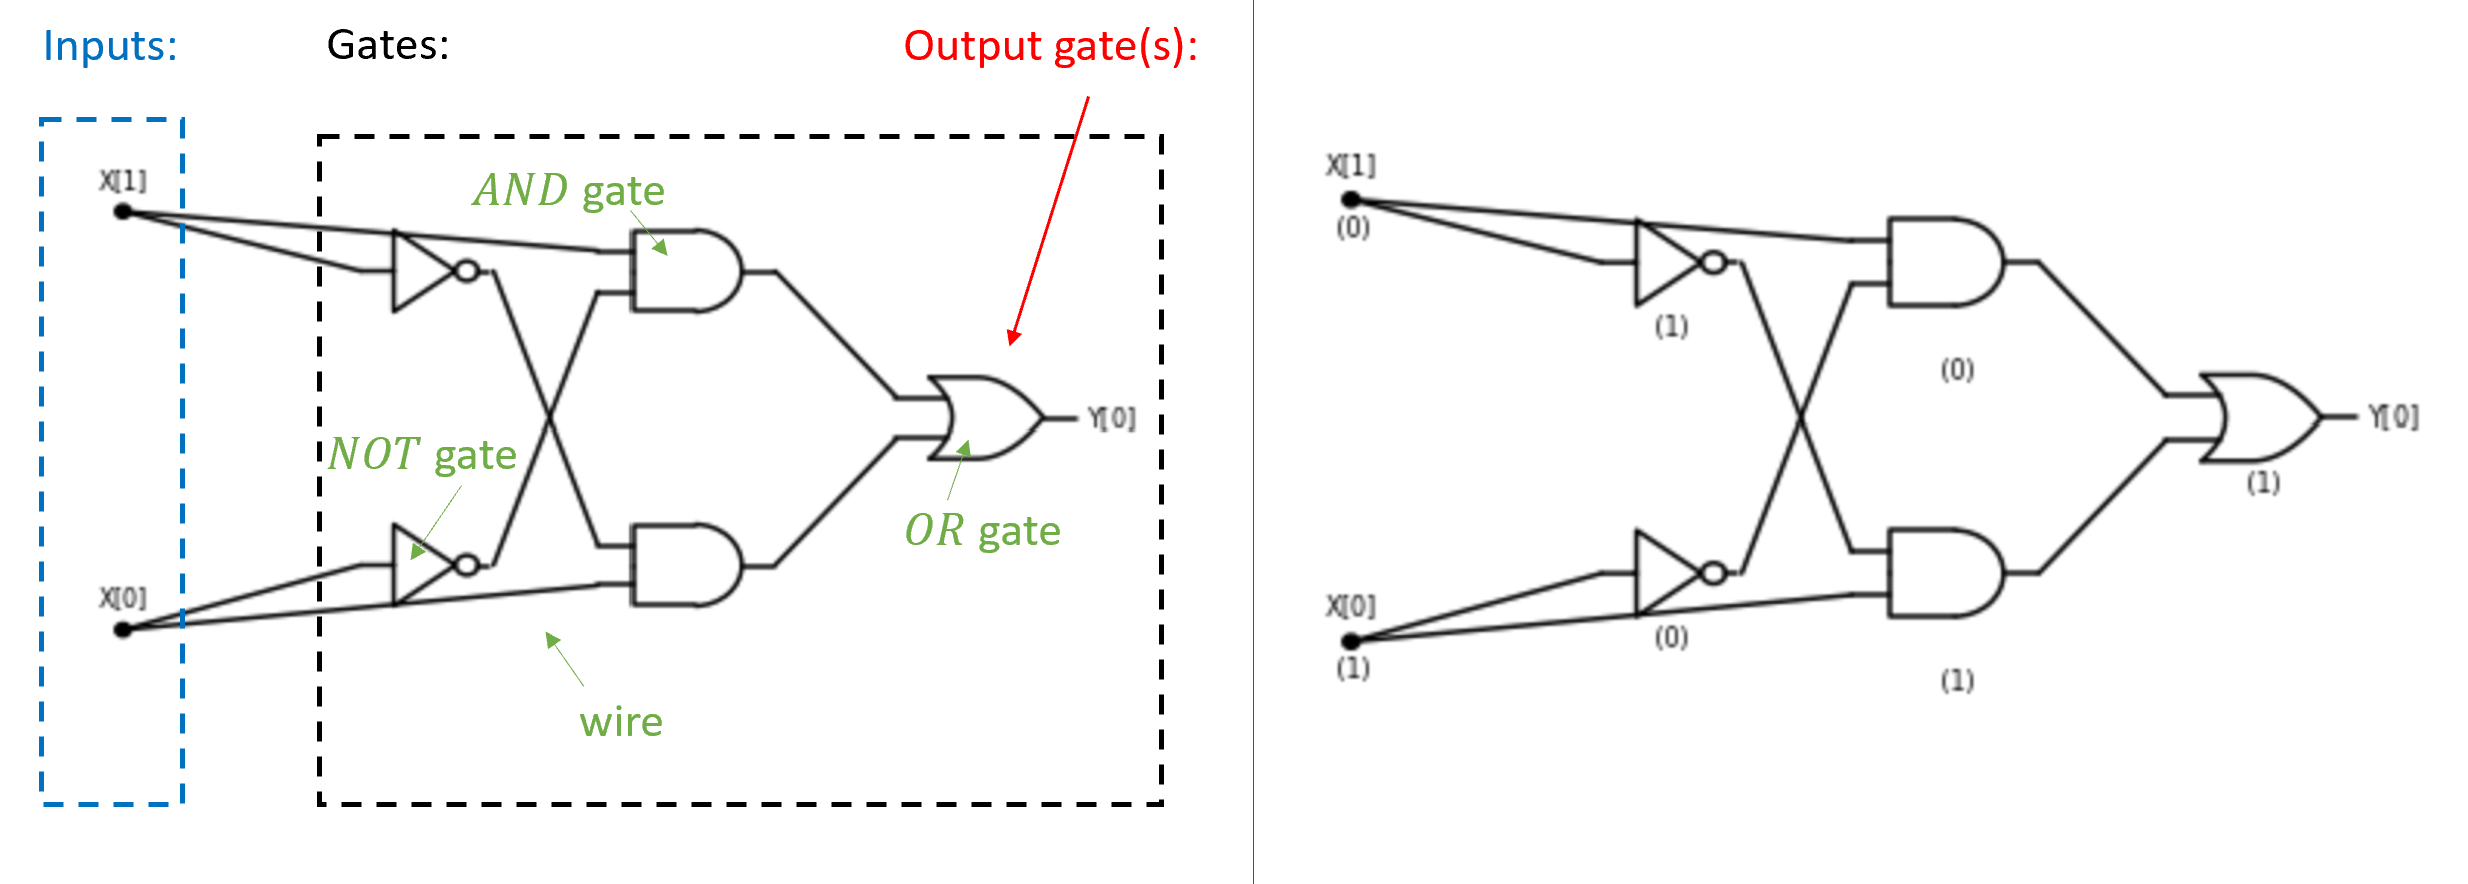
\includegraphics[width=\textwidth, height=0.25\paperheight, keepaspectratio]{../figure/booleancircuit.png}
\caption{A \emph{Boolean Circuit} consists of \emph{gates} that are
connected by \emph{wires} to one another and the \emph{inputs}. The left
side depicts a circuit with \(2\) inputs and \(5\) gates, one of which
is designated the output gate. The right side depicts the evaluation of
this circuit on the input \(x\in \{0,1\}^2\) with \(x_0=1\) and
\(x_1=0\). The value of every gate is obtained by applying the
corresponding function (\(\ensuremath{\mathit{AND}}\),
\(\ensuremath{\mathit{OR}}\), or \(\ensuremath{\mathit{NOT}}\)) to
values on the wire(s) that enter it. The output of the circuit on a
given input is the value of the output gate(s). In this case, the
circuit computes the \(\ensuremath{\mathit{XOR}}\) function and hence it
outputs \(1\) on the input \(10\).}
\label{boolancircfig}
\end{figure}

\hypertarget{allequalex}{}
\begin{solvedexercise}[All equal function] \label[solvedexercise]{allequalex}

Define \(\ensuremath{\mathit{ALLEQ}}:\{0,1\}^4 \rightarrow \{0,1\}\) to
be the function that on input \(x\in \{0,1\}^4\) outputs \(1\) if and
only if \(x_0=x_1=x_2=x_3\). Give a Boolean circuit for computing
\(\ensuremath{\mathit{ALLEQ}}\).

\end{solvedexercise}

\begin{solution} \label[solution]{Another-way-to-describe-t}

Another way to describe the function \(\ensuremath{\mathit{ALLEQ}}\) is
that it outputs \(1\) on an input \(x\in \{0,1\}^4\) if and only if
\(x = 0^4\) or \(x=1^4\). We can phrase the condition \(x=1^4\) as
\(x_0 \wedge x_1 \wedge x_2 \wedge x_3\) which can be computed using
three AND gates. Similarly we can phrase the condition \(x=0^4\) as
\(\overline{x}_0 \wedge \overline{x}_1 \wedge \overline{x}_2 \wedge \overline{x}_3\)
which can be computed using four NOT gates and three AND gates. The
output of \(\ensuremath{\mathit{ALLEQ}}\) is the OR of these two
conditions, which results in the circuit of 4 NOT gates, 6 AND gates,
and one OR gate presented in \cref{allequalfig}.

\end{solution}


\begin{marginfigure}
\centering
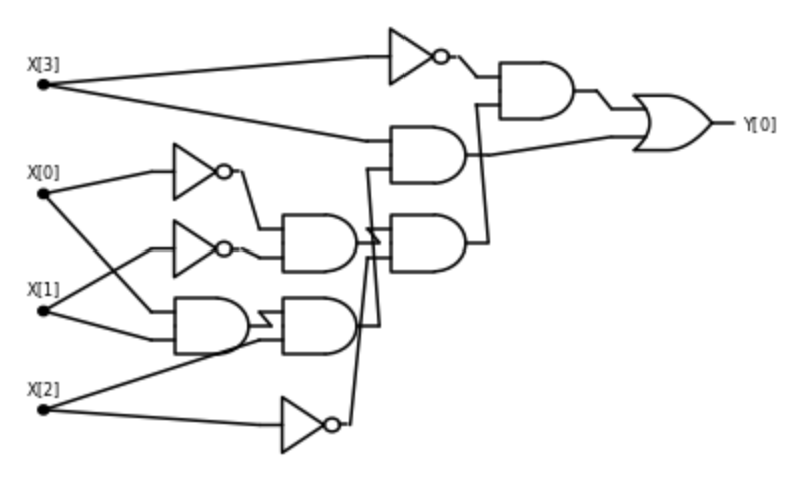
\includegraphics[width=\linewidth, height=1.5in, keepaspectratio]{../figure/allequalcirc2.png}
\caption{A Boolean circuit for computing the \emph{all equal} function
\(\ensuremath{\mathit{ALLEQ}}:\{0,1\}^4 \rightarrow \{0,1\}\) that
outputs \(1\) on \(x\in \{0,1\}^4\) if and only if \(x_0=x_1=x_2=x_3\).}
\label{allequalfig}
\end{marginfigure}

\subsection{Boolean circuits: a formal
definition}\label{Boolean-circuits-a-formal}

We defined Boolean circuits informally as obtained by connecting
\emph{AND}, \emph{OR}, and \emph{NOT} gates via wires so as to produce
an output from an input. However, to be able to prove theorems about the
existence or non-existence of Boolean circuits for computing various
functions we need to:

\begin{enumerate}
\def\labelenumi{\arabic{enumi}.}
\item
  Formally define a Boolean circuit as a mathematical object.
\item
  Formally define what it means for a circuit \(C\) to compute a
  function \(f\).
\end{enumerate}

We now proceed to do so. We will define a Boolean circuit as a labeled
\emph{Directed Acyclic Graph (DAG)}. The \emph{vertices} of the graph
correspond to the gates and inputs of the circuit, and the \emph{edges}
of the graph correspond to the wires. A wire from an input or gate \(u\)
to a gate \(v\) in the circuit corresponds to a directed edge between
the corresponding vertices. The inputs are vertices with no incoming
edges, while each gate has the appropriate number of incoming edges
based on the function it computes. (That is, \emph{AND} and \emph{OR}
gates have two in-neighbors, while \emph{NOT} gates have one
in-neighbor.) The formal definition is as follows (see also
\cref{generalcircuitfig}):


\begin{figure}
\centering
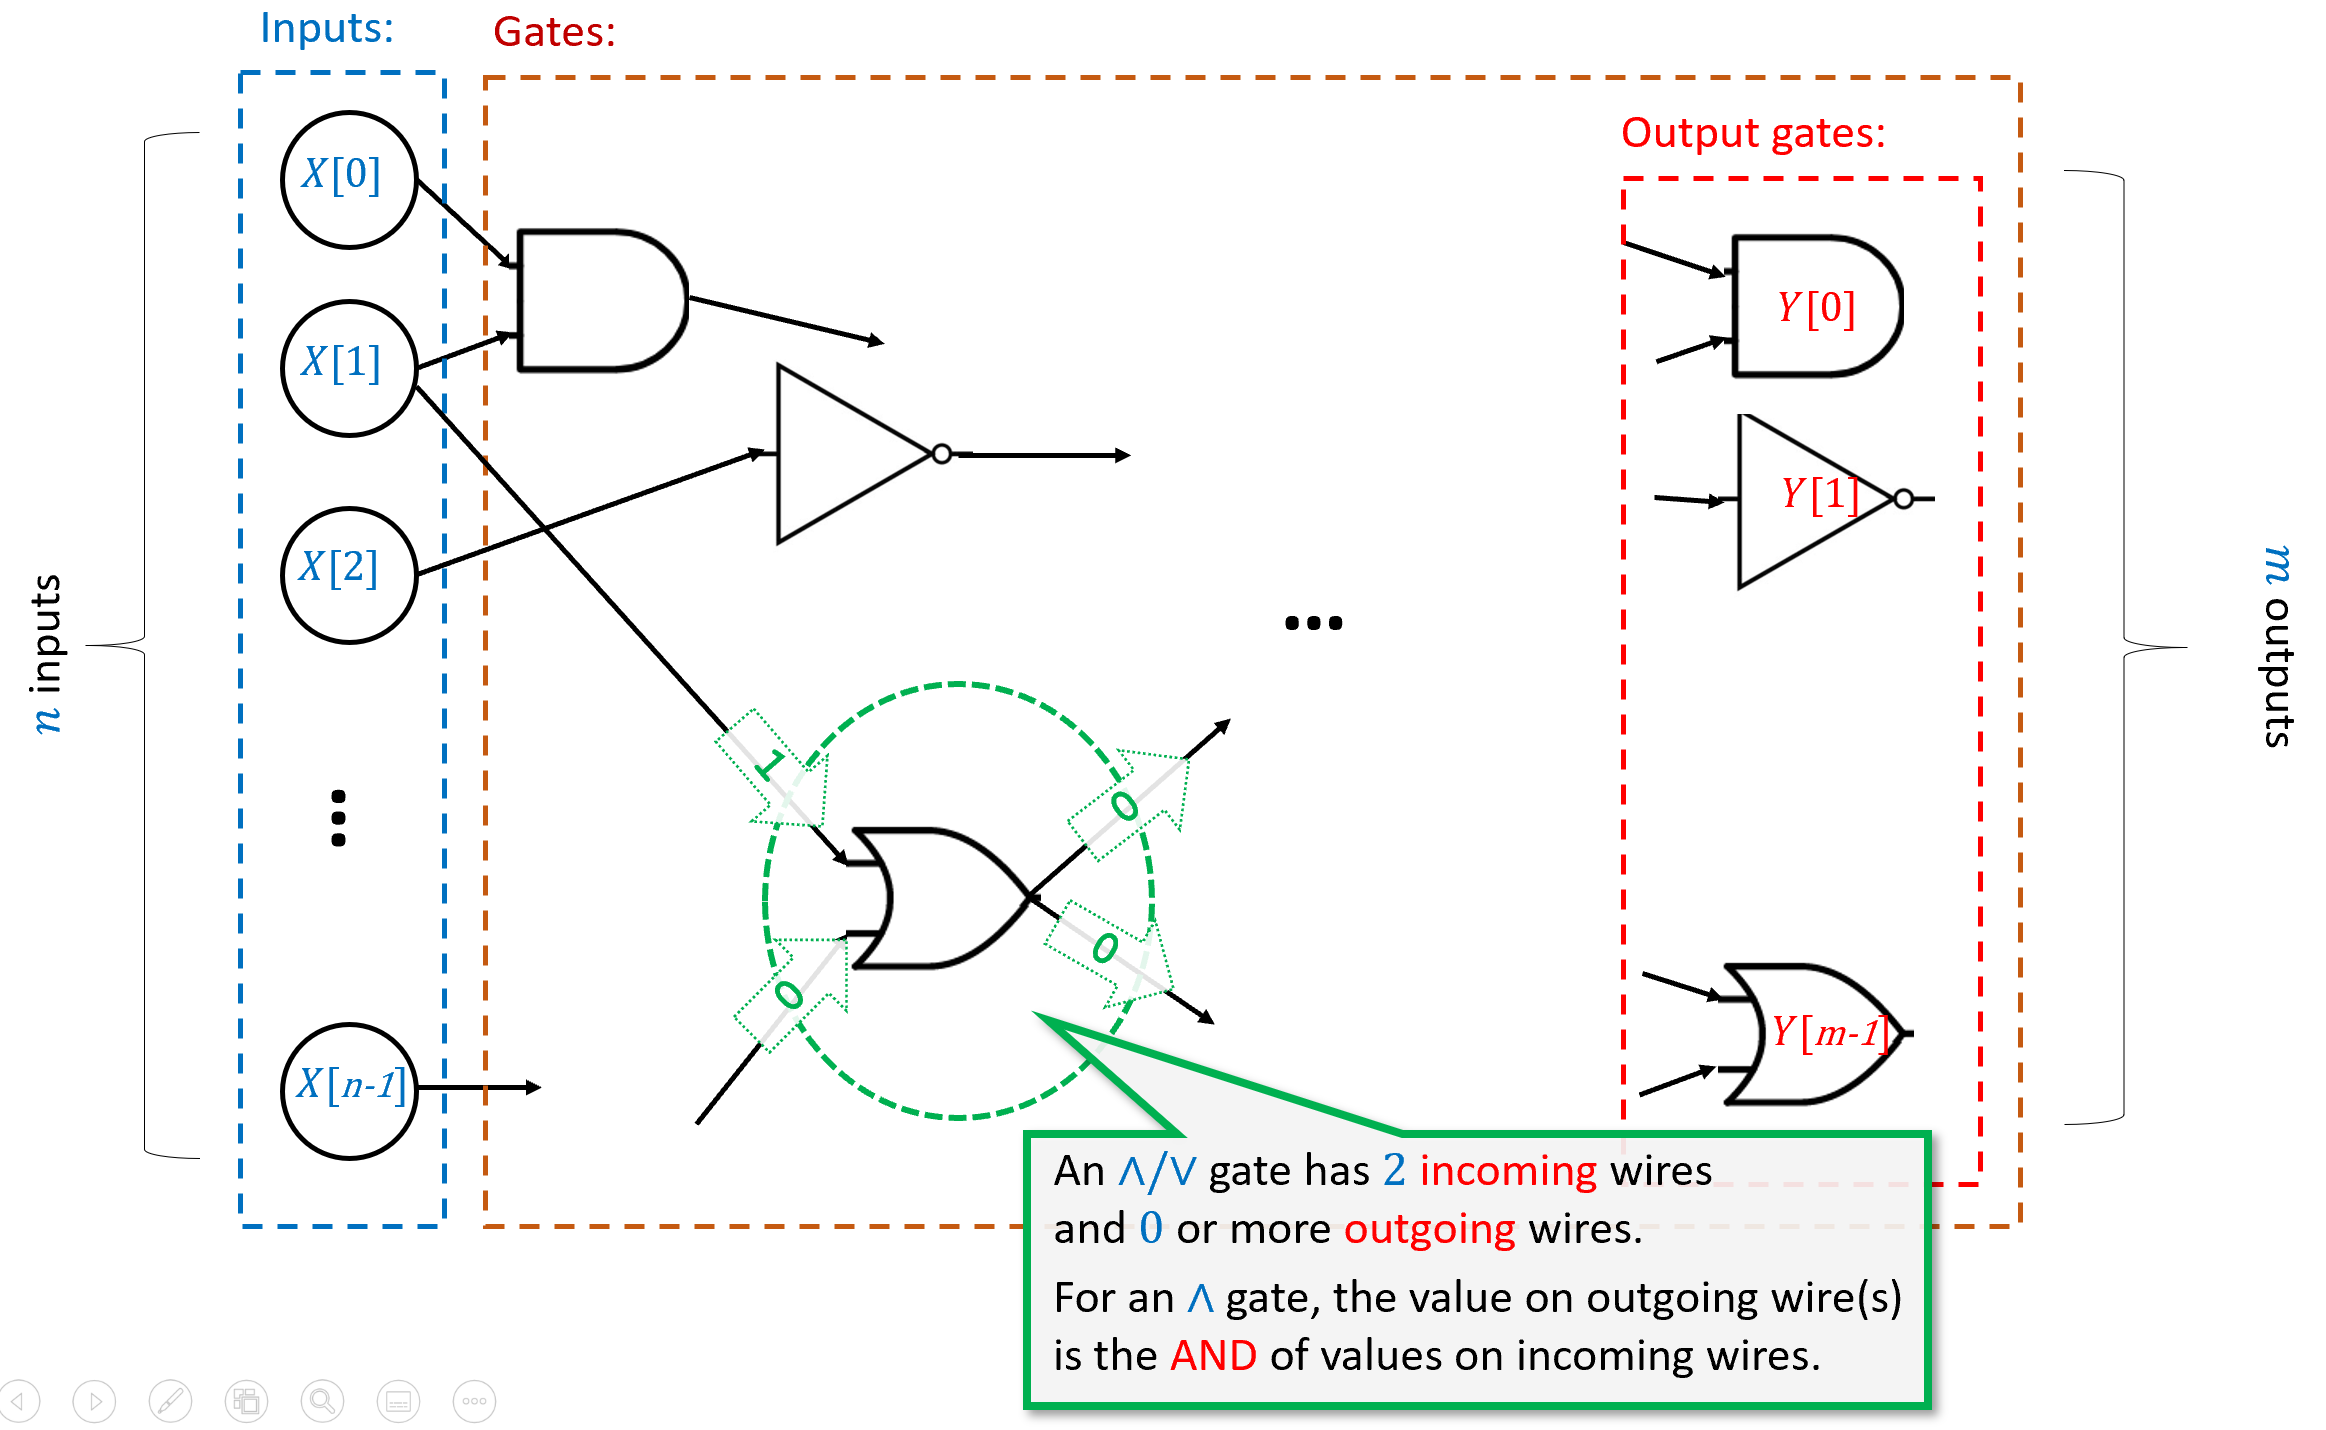
\includegraphics[width=\textwidth, height=0.25\paperheight, keepaspectratio]{../figure/generalcircuit.png}
\caption{A \emph{Boolean Circuit} is a labeled directed acyclic graph
(DAG). It has \(n\) \emph{input} vertices, which are marked with
\texttt{X[}\(0\)\texttt{]},\(\ldots\), \texttt{X[}\(n-1\)\texttt{]} and
have no incoming edges, and the rest of the vertices are \emph{gates}.
\emph{AND}, \emph{OR}, and \emph{NOT} gates have two, two, and one
incoming edges, respectively. If the circuit has \(m\) outputs, then
\(m\) of the gates are known as \emph{outputs} and are marked with
\texttt{Y[}\(0\)\texttt{]},\(\ldots\),\texttt{Y[}\(m-1\)\texttt{]}. When
we evaluate a circuit \(C\) on an input \(x\in \{0,1\}^n\), we start by
setting the value of the input vertices to \(x_0,\ldots,x_{n-1}\) and
then propagate the values, assigning to each gate \(g\) the result of
applying the operation of \(g\) to the values of \(g\)'s in-neighbors.
The output of the circuit is the value assigned to the output gates.}
\label{generalcircuitfig}
\end{figure}

\hypertarget{booleancircdef}{}
\begin{definition}[Boolean Circuits] \label[definition]{booleancircdef}

Let \(n,m,s\) be positive integers with \(s \geq m\). A \emph{Boolean
circuit} with \(n\) inputs, \(m\) outputs, and \(s\) gates, is a labeled
directed acyclic graph (DAG) \(G=(V,E)\) with \(s+n\) vertices
satisfying the following properties:

\begin{itemize}
\item
  Exactly \(n\) of the vertices have no in-neighbors. These vertices are
  known as \emph{inputs} and are labeled with the \(n\) labels
  \texttt{X[}\(0\)\texttt{]}, \(\ldots\), \texttt{X[}\(n-1\)\texttt{]}.
  Each input has at least one out-neighbor.
\item
  The other \(s\) vertices are known as \emph{gates}. Each gate is
  labeled with \(\wedge\), \(\vee\) or \(\neg\). Gates labeled with
  \(\wedge\) (\emph{AND}) or \(\vee\) (\emph{OR}) have two in-neighbors.
  Gates labeled with \(\neg\) (\emph{NOT}) have one in-neighbor. We will
  allow parallel edges.\footnote{Having parallel edges means an AND or
    OR gate \(u\) can have both its in-neighbors be the same gate \(v\).
    Since
    \(\ensuremath{\mathit{AND}}(a,a)=\ensuremath{\mathit{OR}}(a,a)=a\)
    for every \(a\in \{0,1\}\), such parallel edges don't help in
    computing new values in circuits with AND/OR/NOT gates. However, we
    will see circuits with more general sets of gates later on.}
\item
  Exactly \(m\) of the gates are also labeled with the \(m\) labels
  \texttt{Y[}\(0\)\texttt{]}, \(\ldots\), \texttt{Y[}\(m-1\)\texttt{]}
  (in addition to their label \(\wedge\)/\(\vee\)/\(\neg\)). These are
  known as \emph{outputs}.
\end{itemize}

The \emph{size} of a Boolean circuit is the number of gates it contains.

\end{definition}

\begin{pause} \label[pause]{This-is-a-non-trivial-mat}

This is a non-trivial mathematical definition, so it is worth taking the
time to read it slowly and carefully. As in all mathematical
definitions, we are using a known mathematical object --- a directed
acyclic graph (DAG) --- to define a new object, a Boolean circuit. This
might be a good time to review some of the basic properties of DAGs and
in particular the fact that they can be \emph{topologically sorted}, see
\cref{topsortsec}.

\end{pause}

If \(C\) is a circuit with \(n\) inputs and \(m\) outputs, and
\(x\in \{0,1\}^n\), then we can compute the output of \(C\) on the input
\(x\) in the natural way: assign the input vertices
\texttt{X[}\(0\)\texttt{]}, \(\ldots\), \texttt{X[}\(n-1\)\texttt{]} the
values \(x_0,\ldots,x_{n-1}\), apply each gate on the values of its
in-neighbors, and then output the values that correspond to the output
vertices. Formally, this is defined as follows:

\hypertarget{circuitcomputedef}{}
\begin{definition}[Computing a function via a Boolean circuit] \label[definition]{circuitcomputedef}

Let \(C\) be a Boolean circuit with \(n\) inputs and \(m\) outputs. For
every \(x\in \{0,1\}^n\), the \emph{output} of \(C\) on the input \(x\),
denoted by \(C(x)\), is defined as the result of the following process:

We let \(h:V \rightarrow \N\) be the \emph{minimal layering} of \(C\)
(aka \emph{topological sorting}, see \cref{minimallayeruniquethm}). We
let \(L\) be the maximum layer of \(h\), and for \(\ell=0,1,\ldots,L\)
we do the following:

\begin{itemize}
\item
  For every \(v\) in the \(\ell\)-th layer (i.e., \(v\) such that
  \(h(v)=\ell\)) do:

  \begin{itemize}
  \item
    If \(v\) is an input vertex labeled with \texttt{X[}\(i\)\texttt{]}
    for some \(i\in [n]\), then we assign to \(v\) the value \(x_i\).
  \item
    If \(v\) is a gate vertex labeled with \(\wedge\) and with two
    in-neighbors \(u,w\) then we assign to \(v\) the \emph{AND} of the
    values assigned to \(u\) and \(w\). (Since \(u\) and \(w\) are
    in-neighbors of \(v\), they are in a lower layer than \(v\), and
    hence their values have already been assigned.)
  \item
    If \(v\) is a gate vertex labeled with \(\vee\) and with two
    in-neighbors \(u,w\) then we assign to \(v\) the OR of the values
    assigned to \(u\) and \(w\).
  \item
    If \(v\) is a gate vertex labeled with \(\neg\) and with one
    in-neighbor \(u\) then we assign to \(v\) the negation of the value
    assigned to \(u\).
  \end{itemize}
\item
  The result of this process is the value \(y\in \{0,1\}^m\) such that
  for every \(j\in [m]\), \(y_j\) is the value assigned to the vertex
  with label \texttt{Y[}\(j\)\texttt{]}.
\end{itemize}

Let \(f:\{0,1\}^n \rightarrow \{0,1\}^m\). We say that the circuit \(C\)
\emph{computes} \(f\) if for every \(x\in \{0,1\}^n\), \(C(x)=f(x)\).

\end{definition}

\hypertarget{booleancircuitsremarks}{}
\begin{remark}[Boolean circuits nitpicks (optional)] \label[remark]{booleancircuitsremarks}

In phrasing \cref{booleancircdef}, we've made some technical choices
that are not very important, but will be convenient for us later on.
Having parallel edges means an AND or OR gate \(u\) can have both its
in-neighbors be the same gate \(v\). Since
\(\ensuremath{\mathit{AND}}(a,a)=\ensuremath{\mathit{OR}}(a,a)=a\) for
every \(a\in \{0,1\}\), such parallel edges don't help in computing new
values in circuits with AND/OR/NOT gates. However, we will see circuits
with more general sets of gates later on. The condition that every input
vertex has at least one out-neighbor is also not very important because
we can always add ``dummy gates'' that touch these inputs. However, it
is convenient since it guarantees that (since every gate has at most two
in-neighbors) that the number of inputs in a circuit is never larger
than twice its size.

\end{remark}

\subsection{Equivalence of circuits and straight-line
programs}\label{Equivalence-of-circuits-a}

We have seen two ways to describe how to compute a function \(f\) using
\emph{AND}, \emph{OR} and \emph{NOT}:

\begin{itemize}
\item
  A \emph{Boolean circuit}, defined in \cref{booleancircdef}, computes
  \(f\) by connecting via wires \emph{AND}, \emph{OR}, and \emph{NOT}
  gates to the inputs.
\item
  We can also describe such a computation using a \emph{straight-line
  program} that has lines of the form \texttt{foo = AND(bar,blah)},
  \texttt{foo = OR(bar,blah)} and \texttt{foo = NOT(bar)} where
  \texttt{foo}, \texttt{bar} and \texttt{blah} are variable names. (We
  call this a \emph{straight-line program} since it contains no loops or
  branching (e.g., if/then) statements.)
\end{itemize}

We now formally define the AON-CIRC programming language (``AON'' stands
for \emph{AND}/\emph{OR}/\emph{NOT}; ``CIRC'' stands for \emph{circuit})
which has the above operations, and show that it is equivalent to
Boolean circuits.

\hypertarget{AONcircdef}{}
\begin{definition}[AON-CIRC Programming language] \label[definition]{AONcircdef}

An \emph{AON-CIRC program} is a string of lines of the form
\texttt{foo = AND(bar,blah)}, \texttt{foo = OR(bar,blah)} and
\texttt{foo = NOT(bar)} where \texttt{foo}, \texttt{bar} and
\texttt{blah} are variable names.\footnote{We follow the common
  \href{https://goo.gl/QyHa3b}{programming languages convention} of
  using names such as \texttt{foo}, \texttt{bar}, \texttt{baz},
  \texttt{blah} as stand-ins for generic identifiers. A variable
  identifier in our programming language can be any combination of
  letters, numbers, underscores, and brackets. The
  \href{http://tiny.cc/introtcsappendix}{appendix} contains a full
  formal specification of our programming language.} Variables of the
form \texttt{X[}\(i\)\texttt{]} are known as \emph{input} variables, and
variables of the form \texttt{Y[}\(j\)\texttt{]} are known as
\emph{output} variables. In every line, the variables on the righthand
side of the assignment operators must either be input variables or
variables that have already been assigned a value.

A valid AON-CIRC program \(P\) includes input variables of the form
\texttt{X[}\(0\)\texttt{]},\(\ldots\),\texttt{X[}\(n-1\)\texttt{]} and
output variables of the form \texttt{Y[}\(0\)\texttt{]},\(\ldots\),
\texttt{Y[}\(m-1\)\texttt{]} for some \(n,m \geq 1\). If \(P\) is valid
AON-CIRC program and \(x\in \{0,1\}^n\), then we define the \emph{output
of \(P\) on input \(x\)}, denoted by \(P(x)\), to be the string
\(y\in \{0,1\}^m\) corresponding to the values of the output variables
\texttt{Y[}\(0\)\texttt{]} ,\(\ldots\), \texttt{Y[}\(m-1\)\texttt{]} in
the execution of \(P\) where we initialize the input variables
\texttt{X[}\(0\)\texttt{]},\(\ldots\),\texttt{X[}\(n-1\)\texttt{]} to
the values \(x_0,\ldots,x_{n-1}\).

We say that such an AON-CIRC program \(P\) \emph{computes} a function
\(f:\{0,1\}^n \rightarrow \{0,1\}^m\) if \(P(x)=f(x)\) for every
\(x\in \{0,1\}^n\).

\end{definition}

AON-CIRC is not a practical programming language: it was designed for
pedagogical purposes only, as a way to model computation as composition
of \(\ensuremath{\mathit{AND}}\), \(\ensuremath{\mathit{OR}}\), and
\(\ensuremath{\mathit{NOT}}\). However, AON-CIRC can still be easily
implemented on a computer. The following solved exercise gives an
example of an AON-CIRC program.

\hypertarget{aonforcmpsolved}{}
\begin{solvedexercise} \label[solvedexercise]{aonforcmpsolved}

Consider the following function
\(\ensuremath{\mathit{CMP}}:\{0,1\}^4 \rightarrow \{0,1\}\) that on four
input bits \(a,b,c,d\in \{0,1\}\), outputs \(1\) iff the number
represented by \((a,b)\) is larger than the number represented by
\((c,d)\). That is \(\ensuremath{\mathit{CMP}}(a,b,c,d)=1\) iff
\(2a+b>2c+d\).

Write an AON-CIRC program to compute \(\ensuremath{\mathit{CMP}}\).

\end{solvedexercise}

\begin{solution} \label[solution]{Writing-such-a-program-is}

Writing such a program is tedious but not truly hard. To compare two
numbers we first compare their most significant digit, and then go down
to the next digit and so on and so forth. In this case where the numbers
have just two binary digits, these comparisons are particularly simple.
The number represented by \((a,b)\) is larger than the number
represented by \((c,d)\) if and only if one of the following conditions
happens:

\begin{enumerate}
\def\labelenumi{\arabic{enumi}.}
\tightlist
\item
  The most significant bit \(a\) of \((a,b)\) is larger than the most
  significant bit \(c\) of \((c,d)\).
\end{enumerate}

or

\begin{enumerate}
\def\labelenumi{\arabic{enumi}.}
\setcounter{enumi}{1}
\tightlist
\item
  The two most significant bits \(a\) and \(c\) are equal, but \(b>d\).
\end{enumerate}

Another way to express the same condition is the following: the number
\((a,b)\) is larger than \((c,d)\) iff \(a>c\) \textbf{OR} (\(a\ge c\)
\textbf{AND} \(b>d\)).

For binary digits \(\alpha,\beta\), the condition \(\alpha>\beta\) is
simply that \(\alpha=1\) and \(\beta=0\) or
\(\ensuremath{\mathit{AND}}(\alpha,\ensuremath{\mathit{NOT}}(\beta))=1\),
and the condition \(\alpha\ge\beta\) is simply
\(\ensuremath{\mathit{OR}}(\alpha, \ensuremath{\mathit{NOT}}(\beta))=1\).
Together these observations can be used to give the following AON-CIRC
program to compute \(\ensuremath{\mathit{CMP}}\):

\begin{code}
temp_1 = NOT(X[2])
temp_2 = AND(X[0],temp_1)
temp_3 = OR(X[0],temp_1)
temp_4 = NOT(X[3])
temp_5 = AND(X[1],temp_4)
temp_6 = AND(temp_5,temp_3)
Y[0] = OR(temp_2,temp_6)
\end{code}

We can also present this 8-line program as a circuit with 8 gates, see
\cref{aoncmpfig}.

\end{solution}


\begin{marginfigure}
\centering
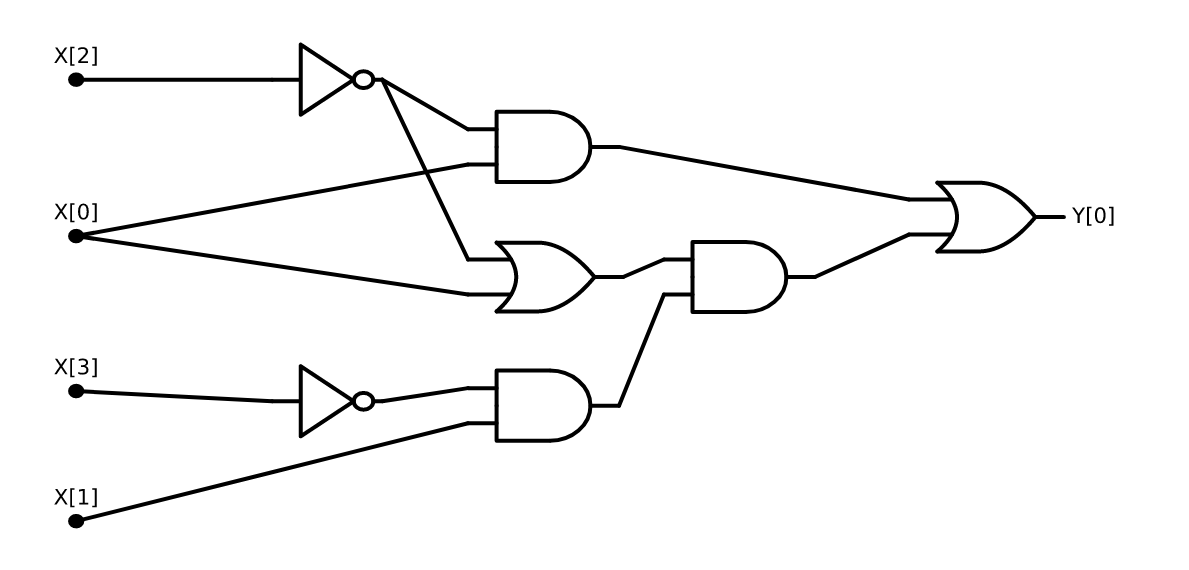
\includegraphics[width=\linewidth, height=1.5in, keepaspectratio]{../figure/comparecircuit.png}
\caption{A circuit for computing the \(\ensuremath{\mathit{CMP}}\)
function. The evaluation of this circuit on \((1,1,1,0)\) yields the
output \(1\), since the number \(3\) (represented in binary as \(11\))
is larger than the number \(2\) (represented in binary as \(10\)).}
\label{aoncmpfig}
\end{marginfigure}

It turns out that AON-CIRC programs and Boolean circuits have exactly
the same power:

\hypertarget{slcircuitequivthm}{}
\begin{theorem}[Equivalence of circuits and straight-line programs] \label[theorem]{slcircuitequivthm}

Let \(f:\{0,1\}^n \rightarrow \{0,1\}^m\) and \(s \geq m\) be some
number. Then \(f\) is computable by a Boolean circuit of \(s\) gates if
and only if \(f\) is computable by an AON-CIRC program of \(s\) lines.

\end{theorem}

\begin{proofidea} \label[proofidea]{The-idea-is-simple---AON-}

The idea is simple - AON-CIRC programs and Boolean circuits are just
different ways of describing the exact same computational process. For
example, an \emph{AND} gate in a Boolean circuit corresponding to
computing the \emph{AND} of two previously-computed values. In a
AON-CIRC program this will correspond to the line that stores in a
variable the \texttt{AND} of two previously-computed variables.

\end{proofidea}

\begin{pause} \label[pause]{This-proof-of-crefslcircu}

This proof of \cref{slcircuitequivthm} is simple at heart, but all the
details it contains can make it a little cumbersome to read. You might
be better off trying to work it out yourself before reading it. Our
\href{https://github.com/boazbk/tcscode}{GitHub repository} contains a
``proof by Python'' of \cref{slcircuitequivthm}: implementation of
functions \texttt{circuit2prog} and \texttt{prog2circuits} mapping
Boolean circuits to AON-CIRC programs and vice versa.

\end{pause}

\begin{proof}[Proof of \cref{slcircuitequivthm}] \label[proof]{Let-fn-rightarrow-m-Since}

Let \(f:\{0,1\}^n \rightarrow \{0,1\}^m\). Since the theorem is an ``if
and only if'' statement, to prove it we need to show both directions:
translating an AON-CIRC program that computes \(f\) into a circuit that
computes \(f\), and translating a circuit that computes \(f\) into an
AON-CIRC program that does so.

We start with the first direction. Let \(P\) be an \(s\) line AON-CIRC
that computes \(f\). We define a circuit \(C\) as follows: the circuit
will have \(n\) inputs and \(s\) gates. For every \(i \in [s]\), if the
\(i\)-th line has the form \texttt{foo = AND(bar,blah)} then the
\(i\)-th gate in the circuit will be an AND gate that is connected to
gates \(j\) and \(k\) where \(j\) and \(k\) correspond to the last lines
before \(i\) where the variables \texttt{bar} and \texttt{blah}
(respectively) where written to. (For example, if \(i=57\) and the last
line \texttt{bar} was written to is \(35\) and the last line
\texttt{blah} was written to is \(17\) then the two in-neighbors of gate
\(57\) will be gates \(35\) and \(17\).) If either \texttt{bar} or
\texttt{blah} is an input variable then we connect the gate to the
corresponding input vertex instead. If \texttt{foo} is an output
variable of the form \texttt{Y[}\(j\)\texttt{]} then we add the same
label to the corresponding gate to mark it as an output gate. We do the
analogous operations if the \(i\)-th line involves an \texttt{OR} or a
\texttt{NOT} operation (except that we use the corresponding \emph{OR}
or \emph{NOT} gate, and in the latter case have only one in-neighbor
instead of two). For every input \(x\in \{0,1\}^n\), if we run the
program \(P\) on \(x\), then the value written that is computed in the
\(i\)-th line is exactly the value that will be assigned to the \(i\)-th
gate if we evaluate the circuit \(C\) on \(x\). Hence \(C(x)=P(x)\) for
every \(x\in \{0,1\}^n\).

For the other direction, let \(C\) be a circuit of \(s\) gates and \(n\)
inputs that computes the function \(f\). We sort the gates according to
a topological order and write them as \(v_0,\ldots,v_{s-1}\). We now can
create a program \(P\) of \(s\) lines as follows. For every
\(i\in [s]\), if \(v_i\) is an AND gate with in-neighbors \(v_j,v_k\)
then we will add a line to \(P\) of the form \texttt{temp\_}\(i\)
\texttt{= AND(temp\_}\(j\)\texttt{,temp\_}\(k\)\texttt{)}, unless one of
the vertices is an input vertex or an output gate, in which case we
change this to the form \texttt{X[.]} or \texttt{Y[.]} appropriately.
Because we work in topological ordering, we are guaranteed that the
in-neighbors \(v_j\) and \(v_k\) correspond to variables that have
already been assigned a value. We do the same for OR and NOT gates. Once
again, one can verify that for every input \(x\), the value \(P(x)\)
will equal \(C(x)\) and hence the program computes the same function as
the circuit. (Note that since \(C\) is a valid circuit, per
\cref{booleancircdef}, every input vertex of \(C\) has at least one
out-neighbor and there are exactly \(m\) output gates labeled
\(0,\ldots,m-1\); hence all the variables \texttt{X[0]}, \(\ldots\),
\texttt{X[}\(n-1\)\texttt{]} and \texttt{Y[0]} ,\(\ldots\),
\texttt{Y[}\(m-1\)\texttt{]} will appear in the program \(P\).)

\end{proof}


\begin{marginfigure}
\centering
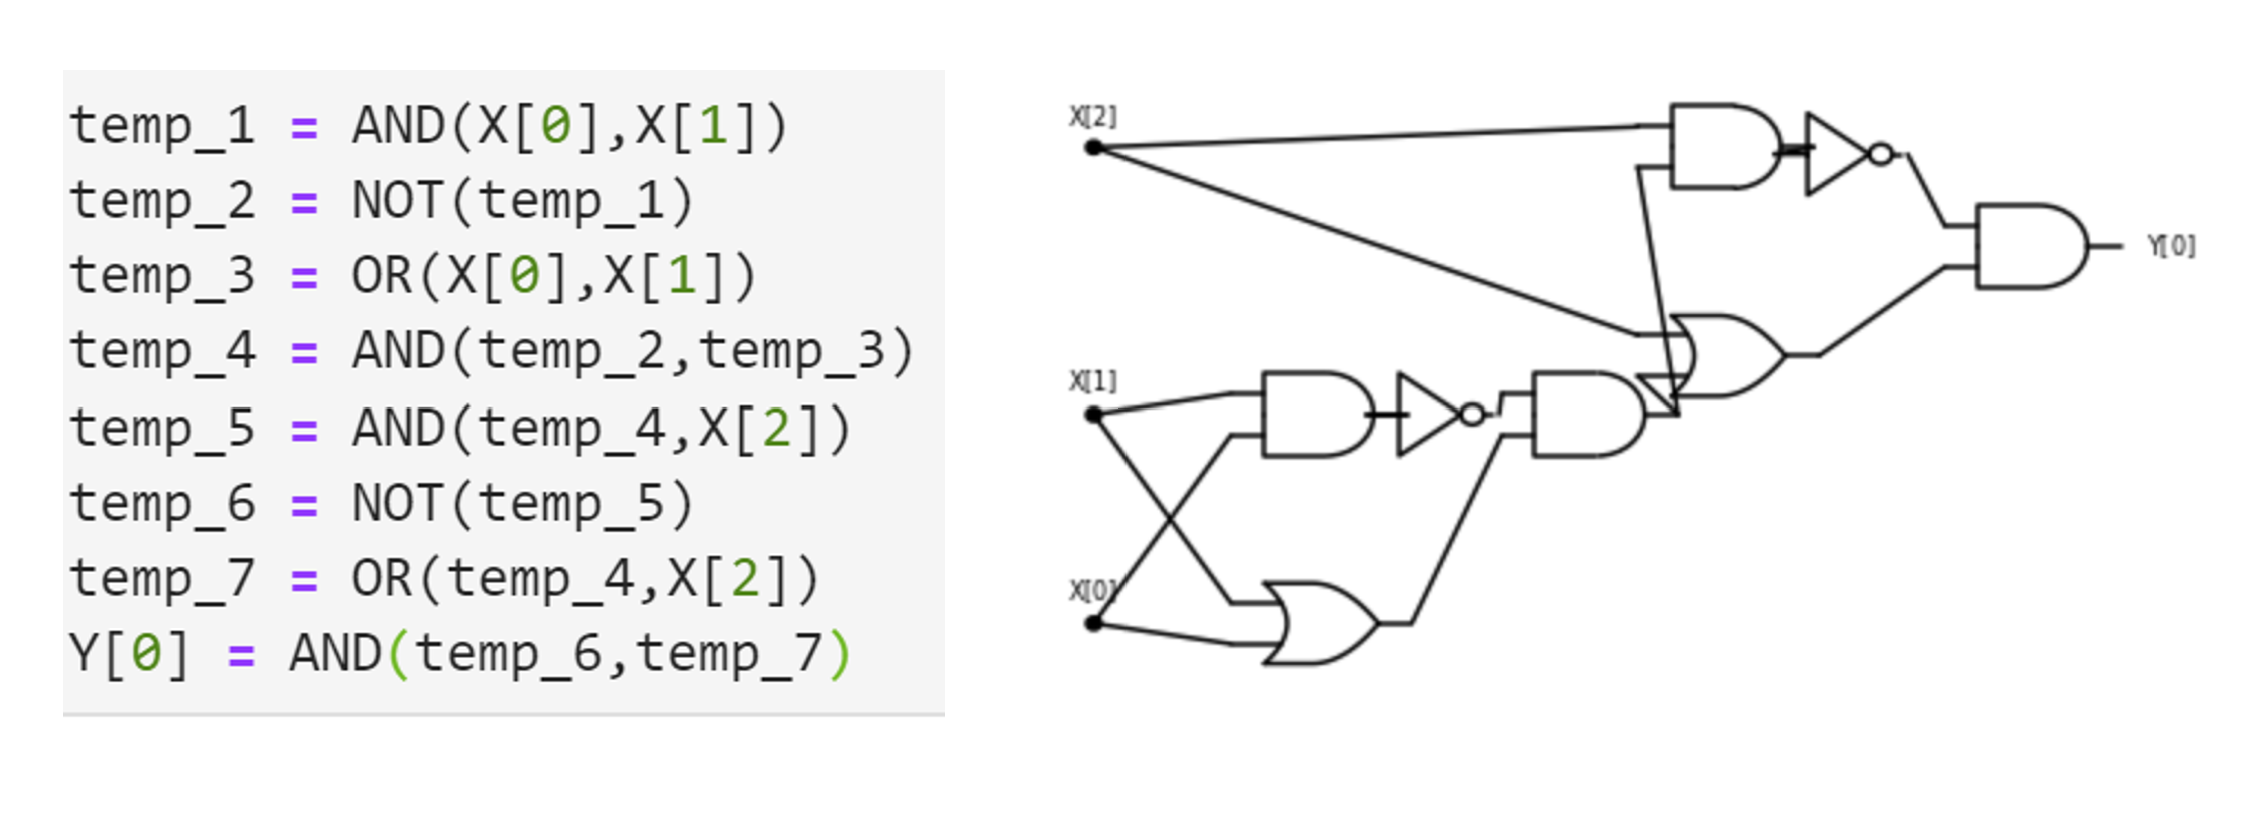
\includegraphics[width=\linewidth, height=1.5in, keepaspectratio]{../figure/aoncircequiv.png}
\caption{Two equivalent descriptions of the same AND/OR/NOT computation
as both an AON program and a Boolean circuit.}
\label{aoncircequivfig}
\end{marginfigure}

\section{Physical implementations of computing devices
(digression)}\label{physicalimplementationsec}

\emph{Computation} is an abstract notion that is distinct from its
physical \emph{implementations}. While most modern computing devices are
obtained by mapping logical gates to semiconductor based transistors,
over history people have computed using a huge variety of mechanisms,
including mechanical systems, gas and liquid (known as \emph{fluidics}),
biological and chemical processes, and even living creatures (e.g., see
\cref{crabfig} or
\href{https://www.youtube.com/watch?v=czk4xgdhdY4}{this video} for how
crabs or slime mold can be used to do computations).

In this section we will review some of these implementations, both so
you can get an appreciation of how it is possible to directly translate
Boolean circuits to the physical world, without going through the entire
stack of architecture, operating systems, and compilers, as well as to
emphasize that silicon-based processors are by no means the only way to
perform computation. Indeed, as we will see in \cref{quantumchap}, a
very exciting recent line of work involves using different media for
computation that would allow us to take advantage of \emph{quantum
mechanical effects} to enable different types of algorithms.


\begin{marginfigure}
\centering
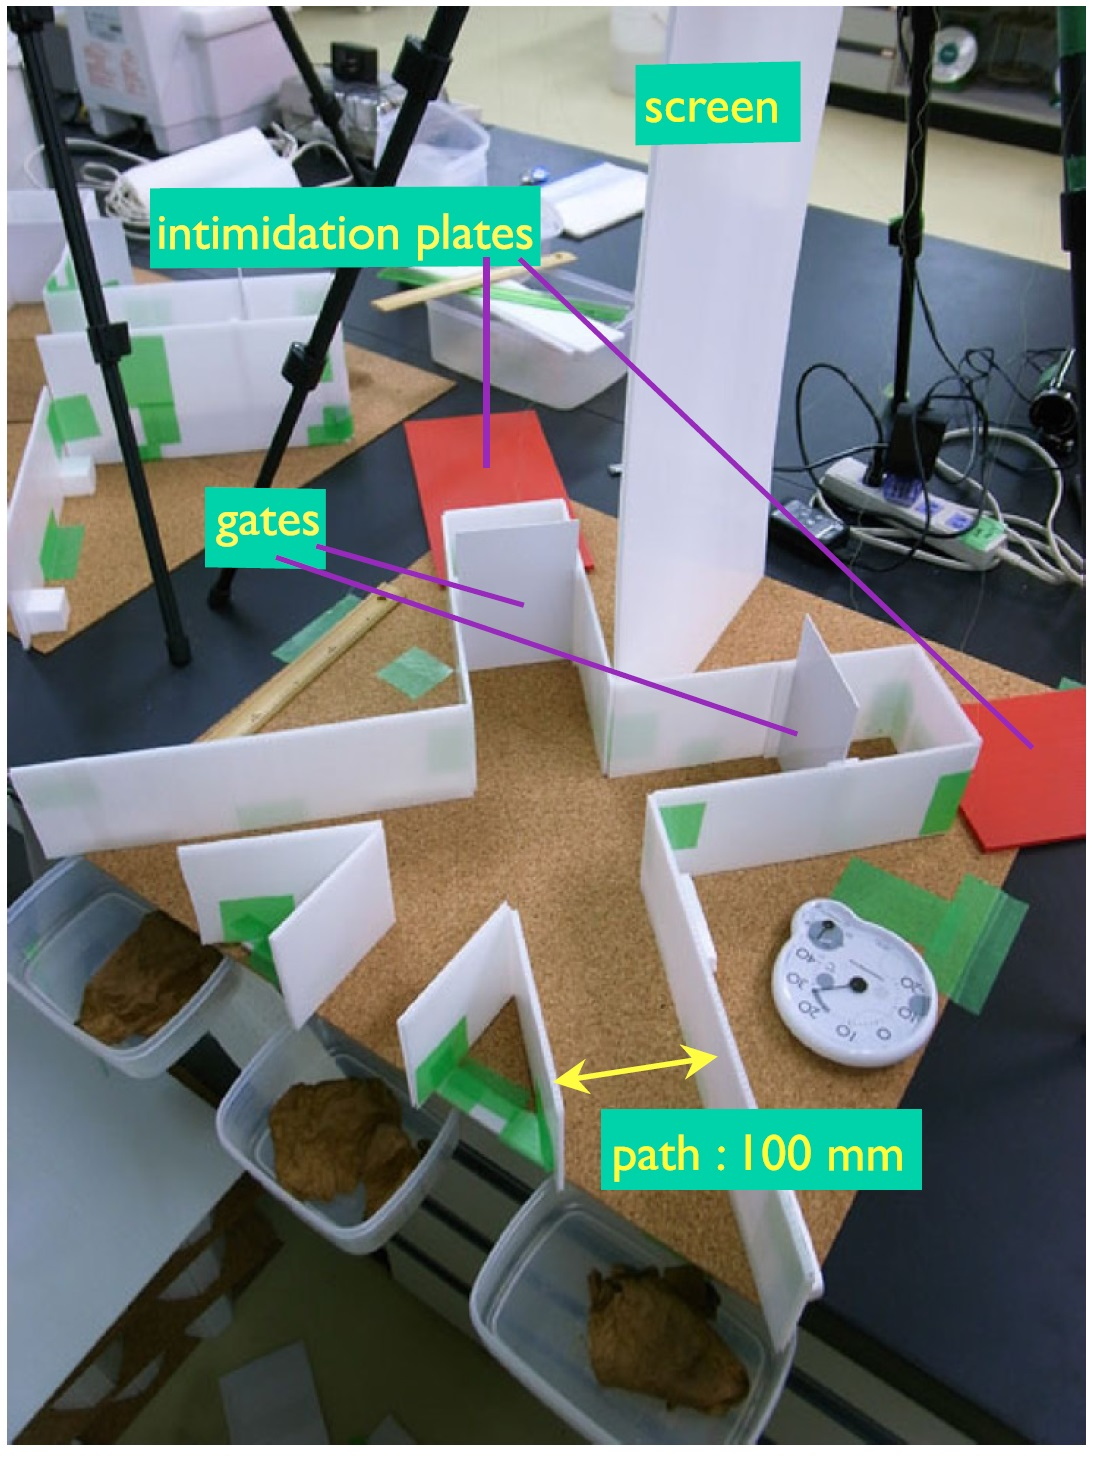
\includegraphics[width=\linewidth, height=1.5in, keepaspectratio]{../figure/crab-gate.jpg}
\caption{Crab-based logic gates from the paper ``Robust soldier-crab
ball gate'' by Gunji, Nishiyama and Adamatzky. This is an example of an
AND gate that relies on the tendency of two swarms of crabs arriving
from different directions to combine to a single swarm that continues in
the average of the directions.}
\label{crabfig}
\end{marginfigure}

\subsection{Transistors}\label{Transistors}

A \emph{transistor} can be thought of as an electric circuit with two
inputs, known as the \emph{source} and the \emph{gate} and an output,
known as the \emph{sink}. The gate controls whether current flows from
the source to the sink. In a \emph{standard transistor}, if the gate is
``ON'' then current can flow from the source to the sink and if it is
``OFF'' then it can't. In a \emph{complementary transistor} this is
reversed: if the gate is ``OFF'' then current can flow from the source
to the sink and if it is ``ON'' then it can't.


\begin{marginfigure}
\centering
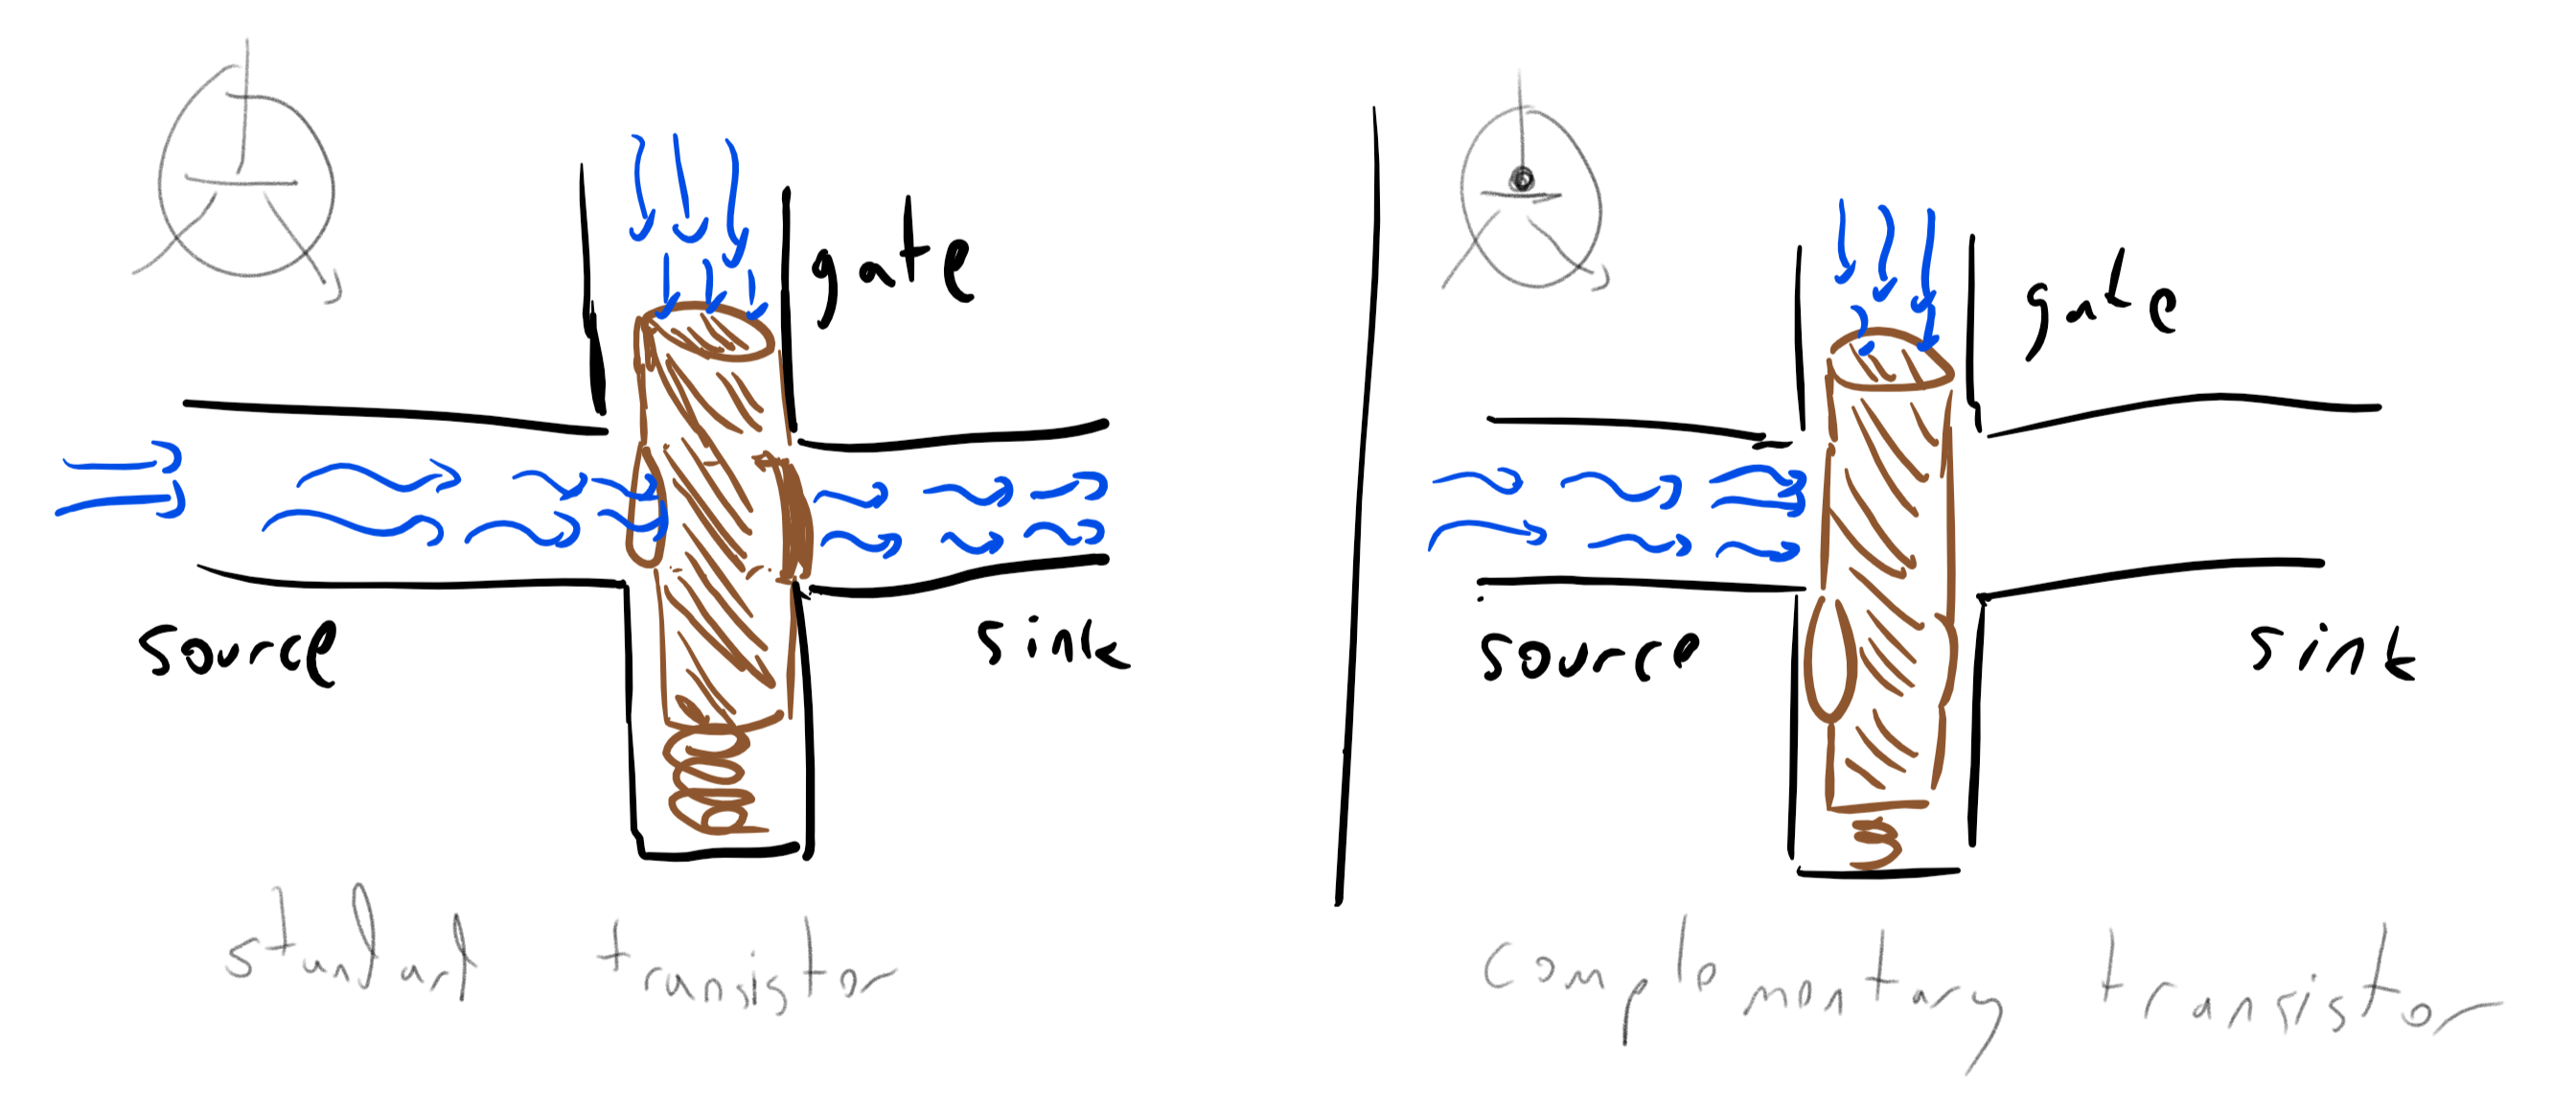
\includegraphics[width=\linewidth, height=1.5in, keepaspectratio]{../figure/transistor_water.png}
\caption{We can implement the logic of transistors using water. The
water pressure from the gate closes or opens a faucet between the source
and the sink.}
\label{transistor-water-fig}
\end{marginfigure}

There are several ways to implement the logic of a transistor. For
example, we can use faucets to implement it using water pressure
(e.g.~\cref{transistor-water-fig}). This might seem as merely a
curiosity, but there is a field known as
\href{https://en.wikipedia.org/wiki/Fluidics}{fluidics} concerned with
implementing logical operations using liquids or gasses. Some of the
motivations include operating in extreme environmental conditions such
as in space or a battlefield, where standard electronic equipment would
not survive.

The standard implementations of transistors use electrical current. One
of the original implementations used \emph{vacuum tubes}. As its name
implies, a vacuum tube is a tube containing nothing (i.e., a vacuum) and
where a priori electrons could freely flow from the source (a wire) to
the sink (a plate). However, there is a gate (a grid) between the two,
where modulating its voltage can block the flow of electrons.

Early vacuum tubes were roughly the size of lightbulbs (and looked very
much like them too). In the 1950's they were supplanted by
\emph{transistors}, which implement the same logic using
\emph{semiconductors} which are materials that normally do not conduct
electricity but whose conductivity can be modified and controlled by
inserting impurities (``doping'') and applying an external electric
field (this is known as the \emph{field effect}). In the 1960's
computers started to be implemented using \emph{integrated circuits}
which enabled much greater density. In 1965, Gordon Moore predicted that
the number of transistors per integrated circuit would double every year
(see \cref{moorefig}), and that this would lead to ``such wonders as
home computers ---or at least terminals connected to a central
computer--- automatic controls for automobiles, and personal portable
communications equipment''. Since then, (adjusted versions of) this
so-called ``Moore's law'' have been running strong, though exponential
growth cannot be sustained forever, and some physical limitations are
already
\href{http://www.nature.com/news/the-chips-are-down-for-moore-s-law-1.19338}{becoming
apparent}.


\begin{marginfigure}
\centering
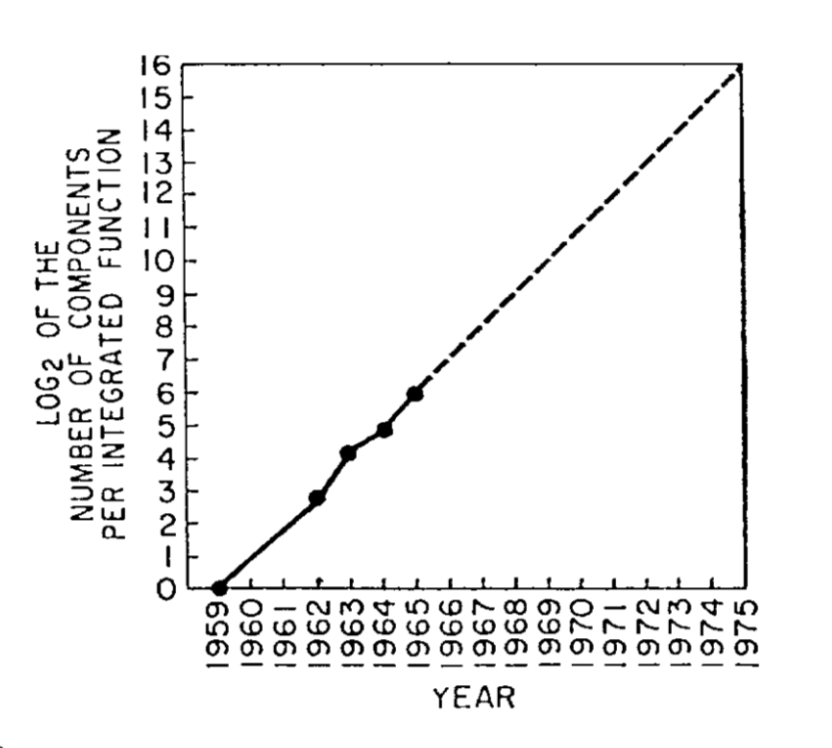
\includegraphics[width=\linewidth, height=1.5in, keepaspectratio]{../figure/gordon_moore.png}
\caption{The number of transistors per integrated circuits from 1959
till 1965 and a prediction that exponential growth will continue for at
least another decade. Figure taken from ``Cramming More Components onto
Integrated Circuits'', Gordon Moore, 1965}
\label{moorefig}
\end{marginfigure}


\begin{marginfigure}
\centering
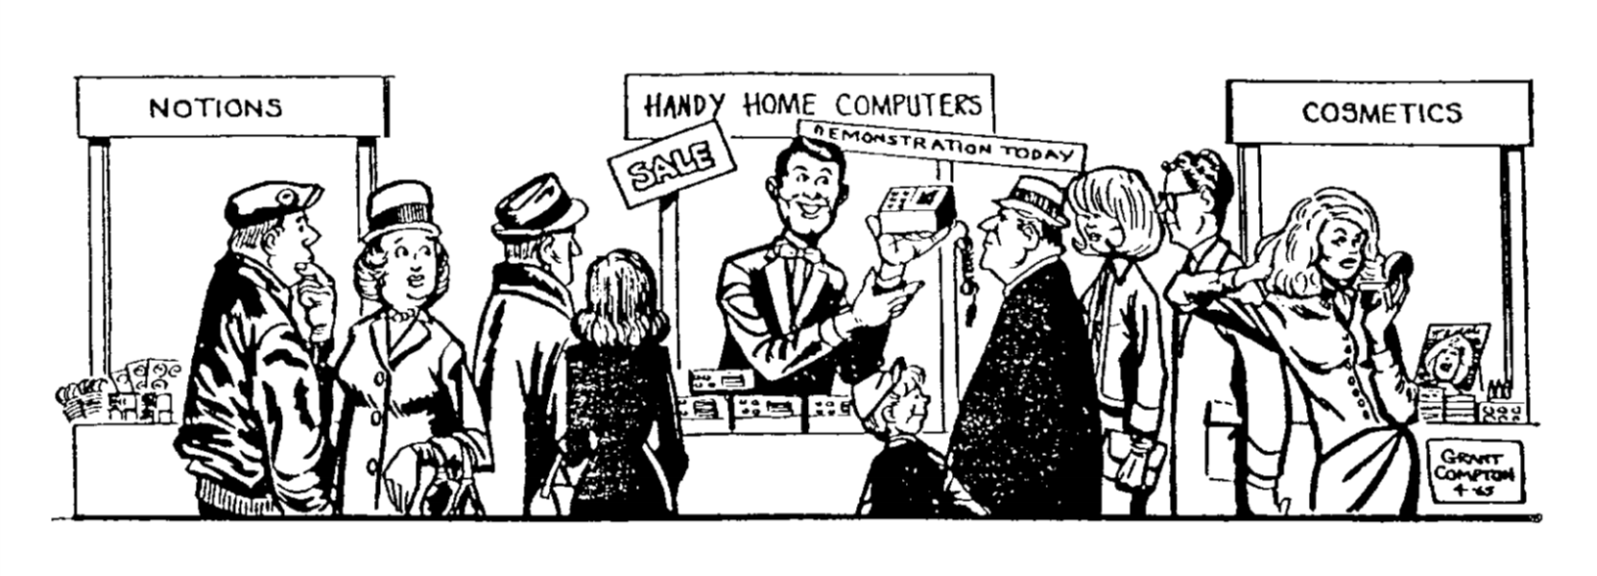
\includegraphics[width=\linewidth, height=1.5in, keepaspectratio]{../figure/moore_cartoon.png}
\caption{Cartoon from Gordon Moore's article ``predicting'' the
implications of radically improving transistor density.}
\label{moore-cartoon-fig}
\end{marginfigure}


\begin{marginfigure}
\centering
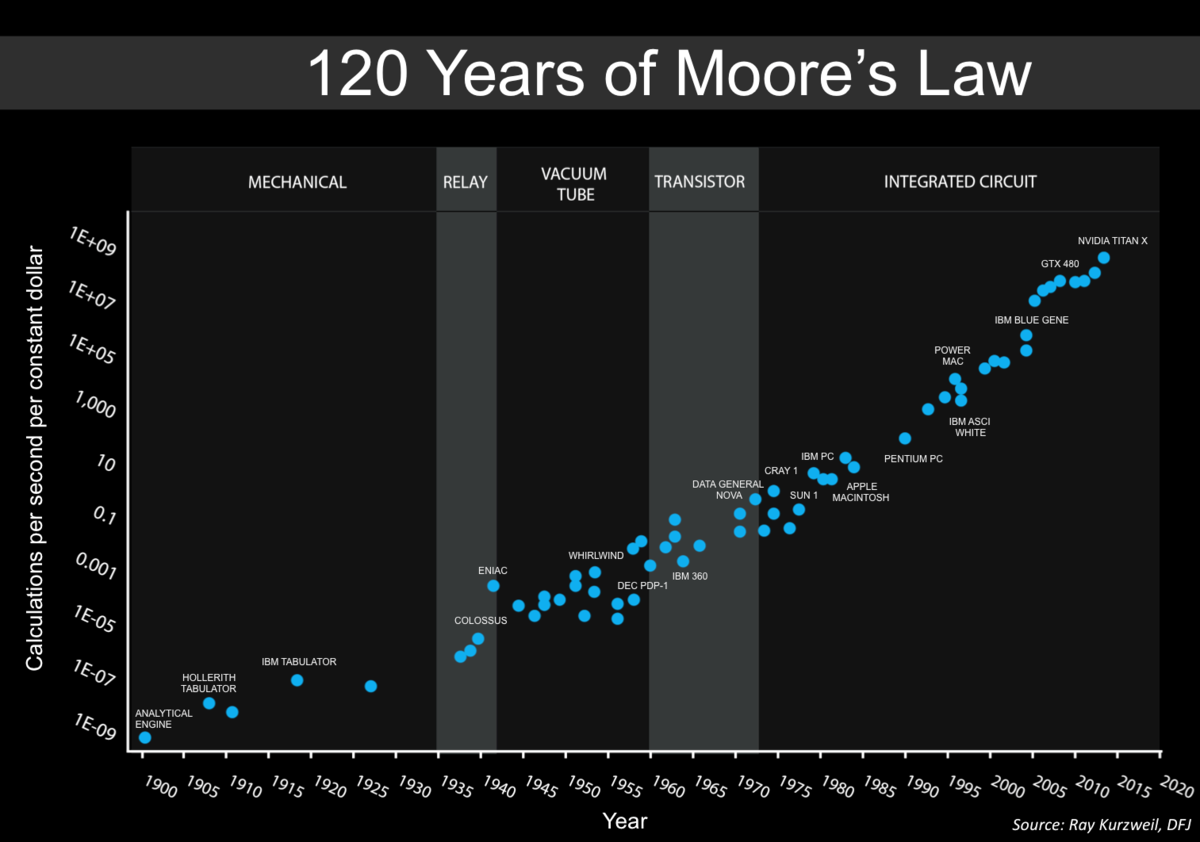
\includegraphics[width=\linewidth, height=1.5in, keepaspectratio]{../figure/1200px-Moore's_Law_over_120_Years.png}
\caption{The exponential growth in computing power over the last 120
years. Graph by Steve Jurvetson, extending a prior graph of Ray
Kurzweil.}
\label{kurzweil-fig}
\end{marginfigure}

\subsection{Logical gates from
transistors}\label{Logical-gates-from-transi}

We can use transistors to implement various Boolean functions such as
\(\ensuremath{\mathit{AND}}\), \(\ensuremath{\mathit{OR}}\), and
\(\ensuremath{\mathit{NOT}}\). For each a two-input gate
\(G:\{0,1\}^2 \rightarrow \{0,1\}\), such an implementation would be a
system with two input wires \(x,y\) and one output wire \(z\), such that
if we identify high voltage with ``\(1\)'' and low voltage with
``\(0\)'', then the wire \(z\) will equal to ``\(1\)'' if and only if
applying \(G\) to the values of the wires \(x\) and \(y\) is \(1\) (see
\cref{logicgatestransistorsfig} and \cref{transistor-nand-fig}). This
means that if there exists a AND/OR/NOT circuit to compute a function
\(g:\{0,1\}^n \rightarrow \{0,1\}^m\), then we can compute \(g\) in the
physical world using transistors as well.


\begin{marginfigure}
\centering
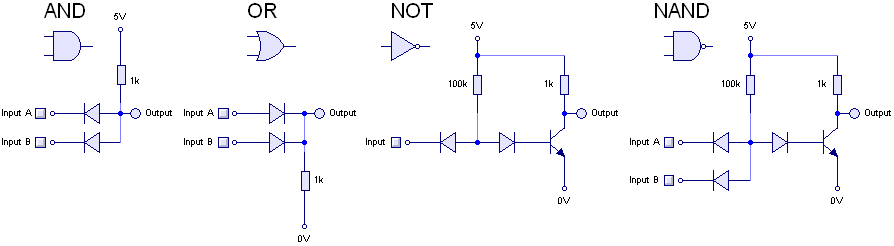
\includegraphics[width=\linewidth, height=1.5in, keepaspectratio]{../figure/DTLLogic.PNG}
\caption{Implementing logical gates using transistors. Figure taken from
\href{http://www.northdownfarm.co.uk/rory/tim/basiclogic.htm}{Rory
Mangles' website}.}
\label{logicgatestransistorsfig}
\end{marginfigure}


\begin{marginfigure}
\centering
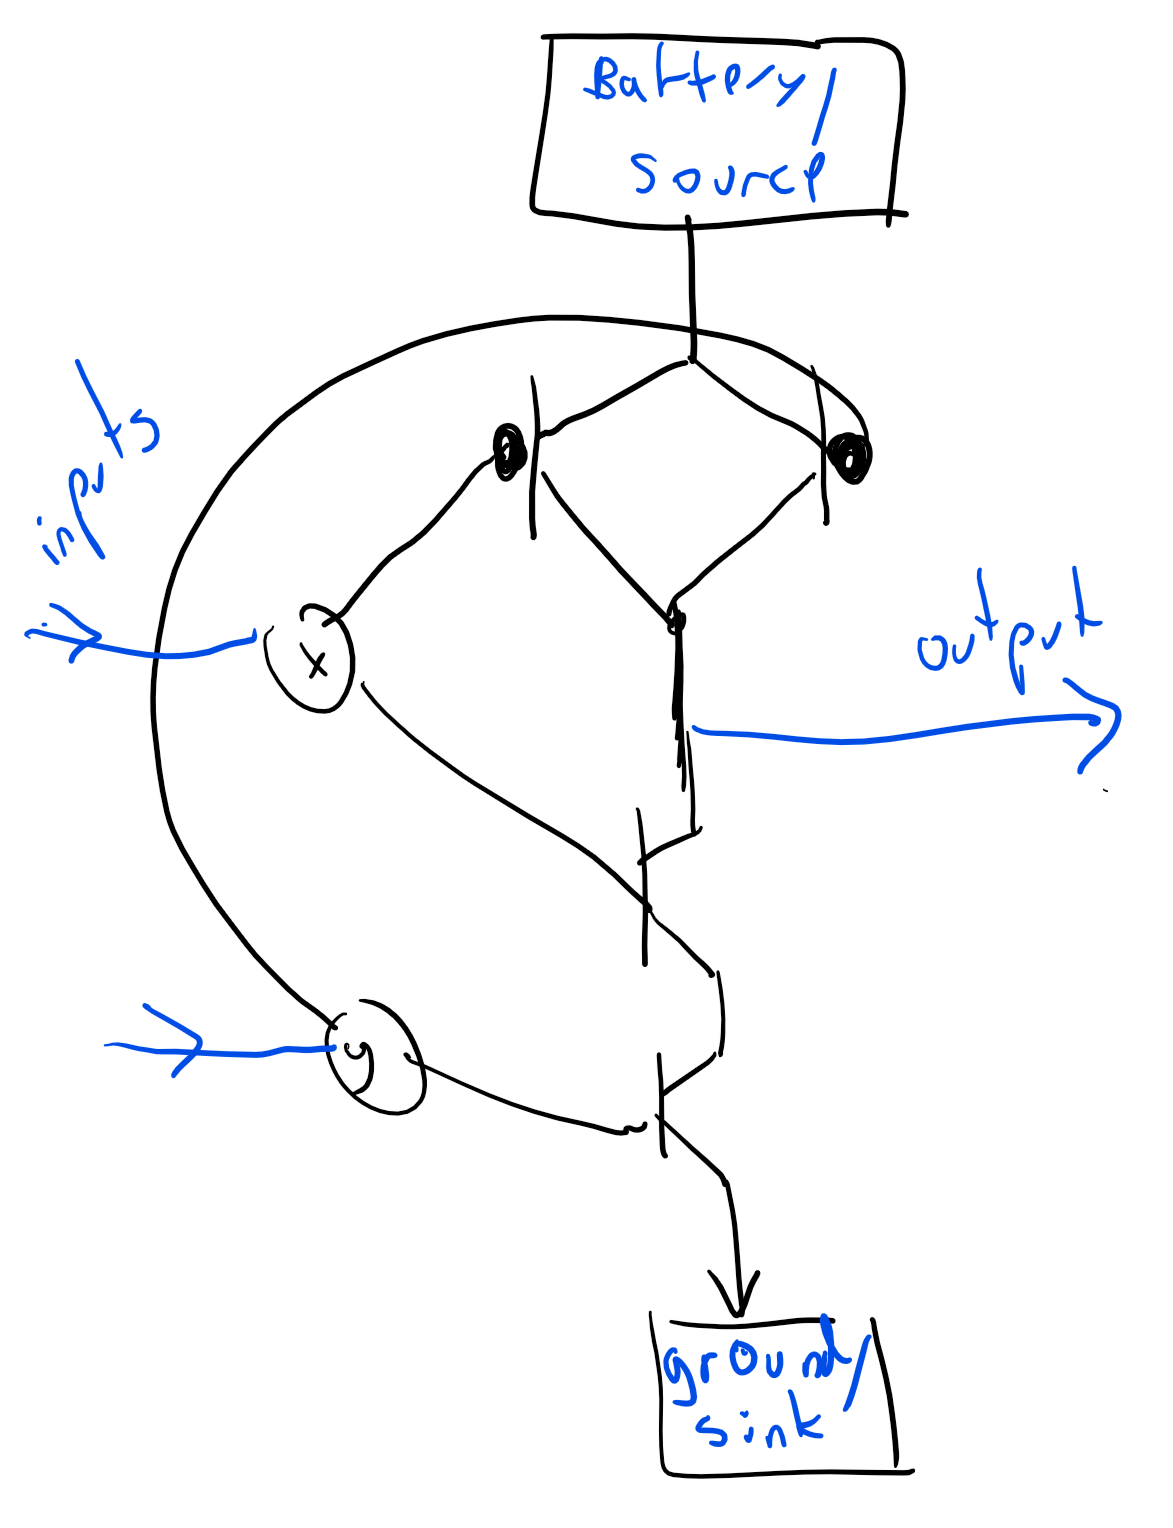
\includegraphics[width=\linewidth, height=1.5in, keepaspectratio]{../figure/nand_transistor.png}
\caption{Implementing a NAND gate (see \cref{nandsec}) using
transistors.}
\label{transistor-nand-fig}
\end{marginfigure}

\subsection{Biological computing}\label{Biological-computing}

Computation can be based on
\href{http://www.nature.com/nrg/journal/v13/n7/full/nrg3197.html}{biological
or chemical systems}. For example the
\href{https://en.wikipedia.org/wiki/Lac_operon}{\emph{lac} operon}
produces the enzymes needed to digest lactose only if the conditions
\(x \wedge (\neg y)\) hold where \(x\) is ``lactose is present'' and
\(y\) is ``glucose is present''. Researchers have managed to
\href{http://science.sciencemag.org/content/340/6132/554?iss=6132}{create
transistors}, and from them logic gates, based on DNA molecules (see
also \cref{transcriptorfig}). One motivation for DNA computing is to
achieve increased parallelism or storage density; another is to create
``smart biological agents'' that could perhaps be injected into bodies,
replicate themselves, and fix or kill cells that were damaged by a
disease such as cancer. Computing in biological systems is not
restricted, of course, to DNA: even larger systems such as
\href{https://www.cs.princeton.edu/~chazelle/pubs/cacm12-natalg.pdf}{flocks
of birds} can be considered as computational processes.


\begin{marginfigure}
\centering
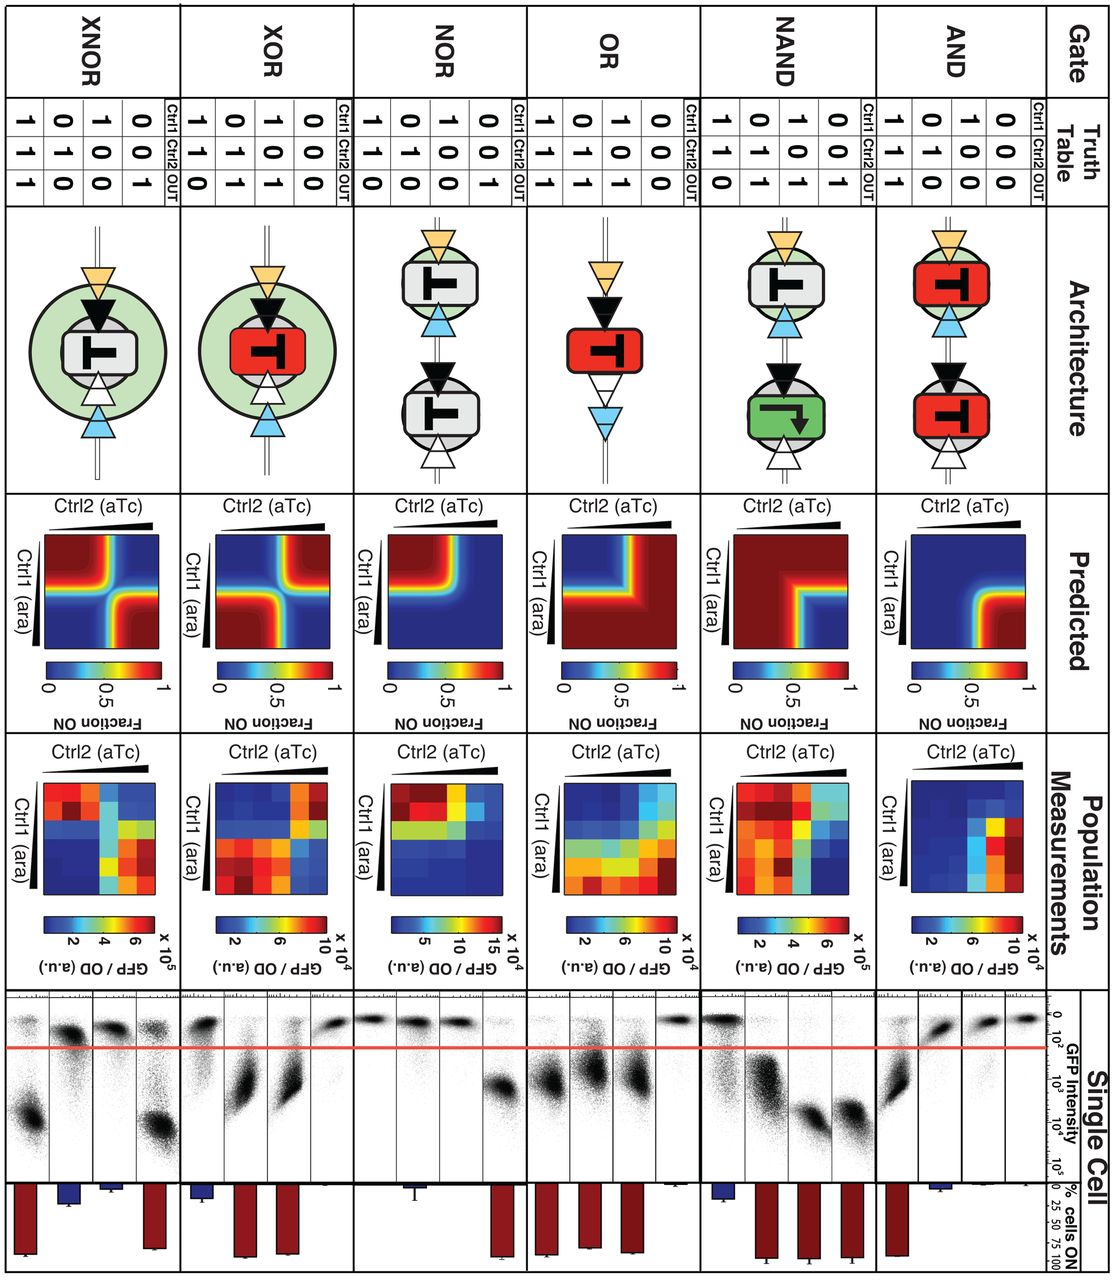
\includegraphics[width=\linewidth, height=1.5in, keepaspectratio]{../figure/transcriptor.jpg}
\caption{Performance of DNA-based logic gates. Figure taken from paper
of
\href{http://science.sciencemag.org/content/early/2013/03/27/science.1232758.full}{Bonnet
et al}, Science, 2013.}
\label{transcriptorfig}
\end{marginfigure}

\subsection{Cellular automata and the game of
life}\label{Cellular-automata-and-the}

\emph{Cellular automata} is a model of a system composed of a sequence
of \emph{cells}, each of which can have a finite state. At each step, a
cell updates its state based on the states of its \emph{neighboring
cells} and some simple rules. As we will discuss later in this book (see
\cref{cellularautomatasec}), cellular automata such as Conway's ``Game
of Life'' can be used to simulate computation gates .


\begin{marginfigure}
\centering
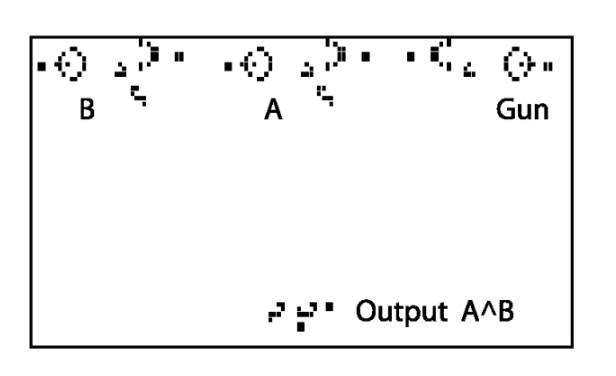
\includegraphics[width=\linewidth, height=1.5in, keepaspectratio]{../figure/game_of_life_and.png}
\caption{An AND gate using a ``Game of Life'' configuration. Figure
taken from
\href{http://www.rennard.org/alife/CollisionBasedRennard.pdf}{Jean-Philippe
Rennard's paper}.}
\label{gameoflifefig}
\end{marginfigure}

\subsection{Neural networks}\label{Neural-networks}

One computation device that we all carry with us is our own
\emph{brain}. Brains have served humanity throughout history, doing
computations that range from distinguishing prey from predators, through
making scientific discoveries and artistic masterpieces, to composing
witty 280 character messages. The exact working of the brain is still
not fully understood, but one common mathematical model for it is a
(very large) \emph{neural network}.

A neural network can be thought of as a Boolean circuit that instead of
\(\ensuremath{\mathit{AND}}\)/\(\ensuremath{\mathit{OR}}\)/\(\ensuremath{\mathit{NOT}}\)
uses some other gates as the basic basis. For example, one particular
basis we can use are \emph{threshold gates}. For every vector
\(w= (w_0,\ldots,w_{k-1})\) of integers and integer \(t\) (some or all
of which could be negative), the \emph{threshold function corresponding
to \(w,t\)} is the function \(T_{w,t}:\{0,1\}^k \rightarrow \{0,1\}\)
that maps \(x\in \{0,1\}^k\) to \(1\) if and only if
\(\sum_{i=0}^{k-1} w_i x_i \geq t\). For example, the threshold function
\(T_{w,t}\) corresponding to \(w=(1,1,1,1,1)\) and \(t=3\) is simply the
majority function \(\ensuremath{\mathit{MAJ}}_5\) on \(\{0,1\}^5\).
Threshold gates can be thought of as an approximation for \emph{neuron
cells} that make up the core of human and animal brains. To a first
approximation, a neuron has \(k\) inputs and a single output, and the
neurons ``fires'' or ``turns on'' its output when those signals pass
some threshold.

Many machine learning algorithms use \emph{artificial neural networks}
whose purpose is not to imitate biology but rather to perform some
computational tasks, and hence are not restricted to threshold or other
biologically-inspired gates. Generally, a neural network is often
described as operating on signals that are real numbers, rather than
\(0/1\) values, and where the output of a gate on inputs
\(x_0,\ldots,x_{k-1}\) is obtained by applying \(f(\sum_i w_i x_i)\)
where \(f:\R \rightarrow \R\) is an
\href{https://goo.gl/p9izfA}{activation function} such as rectified
linear unit (ReLU), Sigmoid, or many others (see
\cref{activationfunctionsfig}). However, for the purposes of our
discussion, all of the above are equivalent (see also
\cref{NANDsfromActivationfunctionex}). In particular we can reduce the
setting of real inputs to binary inputs by representing a real number in
the binary basis, and multiplying the weight of the bit corresponding to
the \(i^{th}\) digit by \(2^i\).


\begin{marginfigure}
\centering
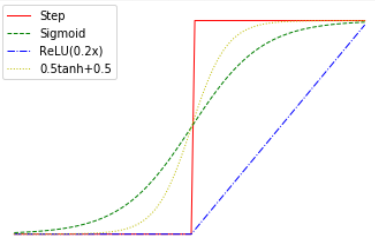
\includegraphics[width=\linewidth, height=1.5in, keepaspectratio]{../figure/activationfuncs.png}
\caption{Common activation functions used in Neural Networks, including
rectified linear units (ReLU), sigmoids, and hyperbolic tangent. All of
those can be thought of as continuous approximations to simple the step
function. All of these can be used to compute the NAND gate (see
\cref{NANDsfromActivationfunctionex}). This property enables neural
networks to (approximately) compute any function that can be computed by
a Boolean circuit.}
\label{activationfunctionsfig}
\end{marginfigure}

\subsection{A computer made from marbles and
pipes}\label{A-computer-made-from-marb}

We can implement computation using many other physical media, without
any electronic, biological, or chemical components. Many suggestions for
\emph{mechanical} computers have been put forward, going back at least
to Gottfried Leibniz' computing machines from the 1670s and Charles
Babbage's 1837 plan for a mechanical
\href{https://en.wikipedia.org/wiki/Analytical_Engine}{``Analytical
Engine''}. As one example, \cref{marblefig} shows a simple
implementation of a NAND (negation of AND, see \cref{nandsec}) gate
using marbles going through pipes. We represent a logical value in
\(\{0,1\}\) by a pair of pipes, such that there is a marble flowing
through exactly one of the pipes. We call one of the pipes the ``\(0\)
pipe'' and the other the ``\(1\) pipe'', and so the identity of the pipe
containing the marble determines the logical value. A NAND gate
corresponds to a mechanical object with two pairs of incoming pipes and
one pair of outgoing pipes, such that for every \(a,b \in \{0,1\}\), if
two marbles are rolling toward the object in the \(a\) pipe of the first
pair and the \(b\) pipe of the second pair, then a marble will roll out
of the object in the \(\ensuremath{\mathit{NAND}}(a,b)\)-pipe of the
outgoing pair. In fact, there is even a commercially-available
educational game that uses marbles as a basis of computing, see
\cref{turingtumblefig}.


\begin{marginfigure}
\centering
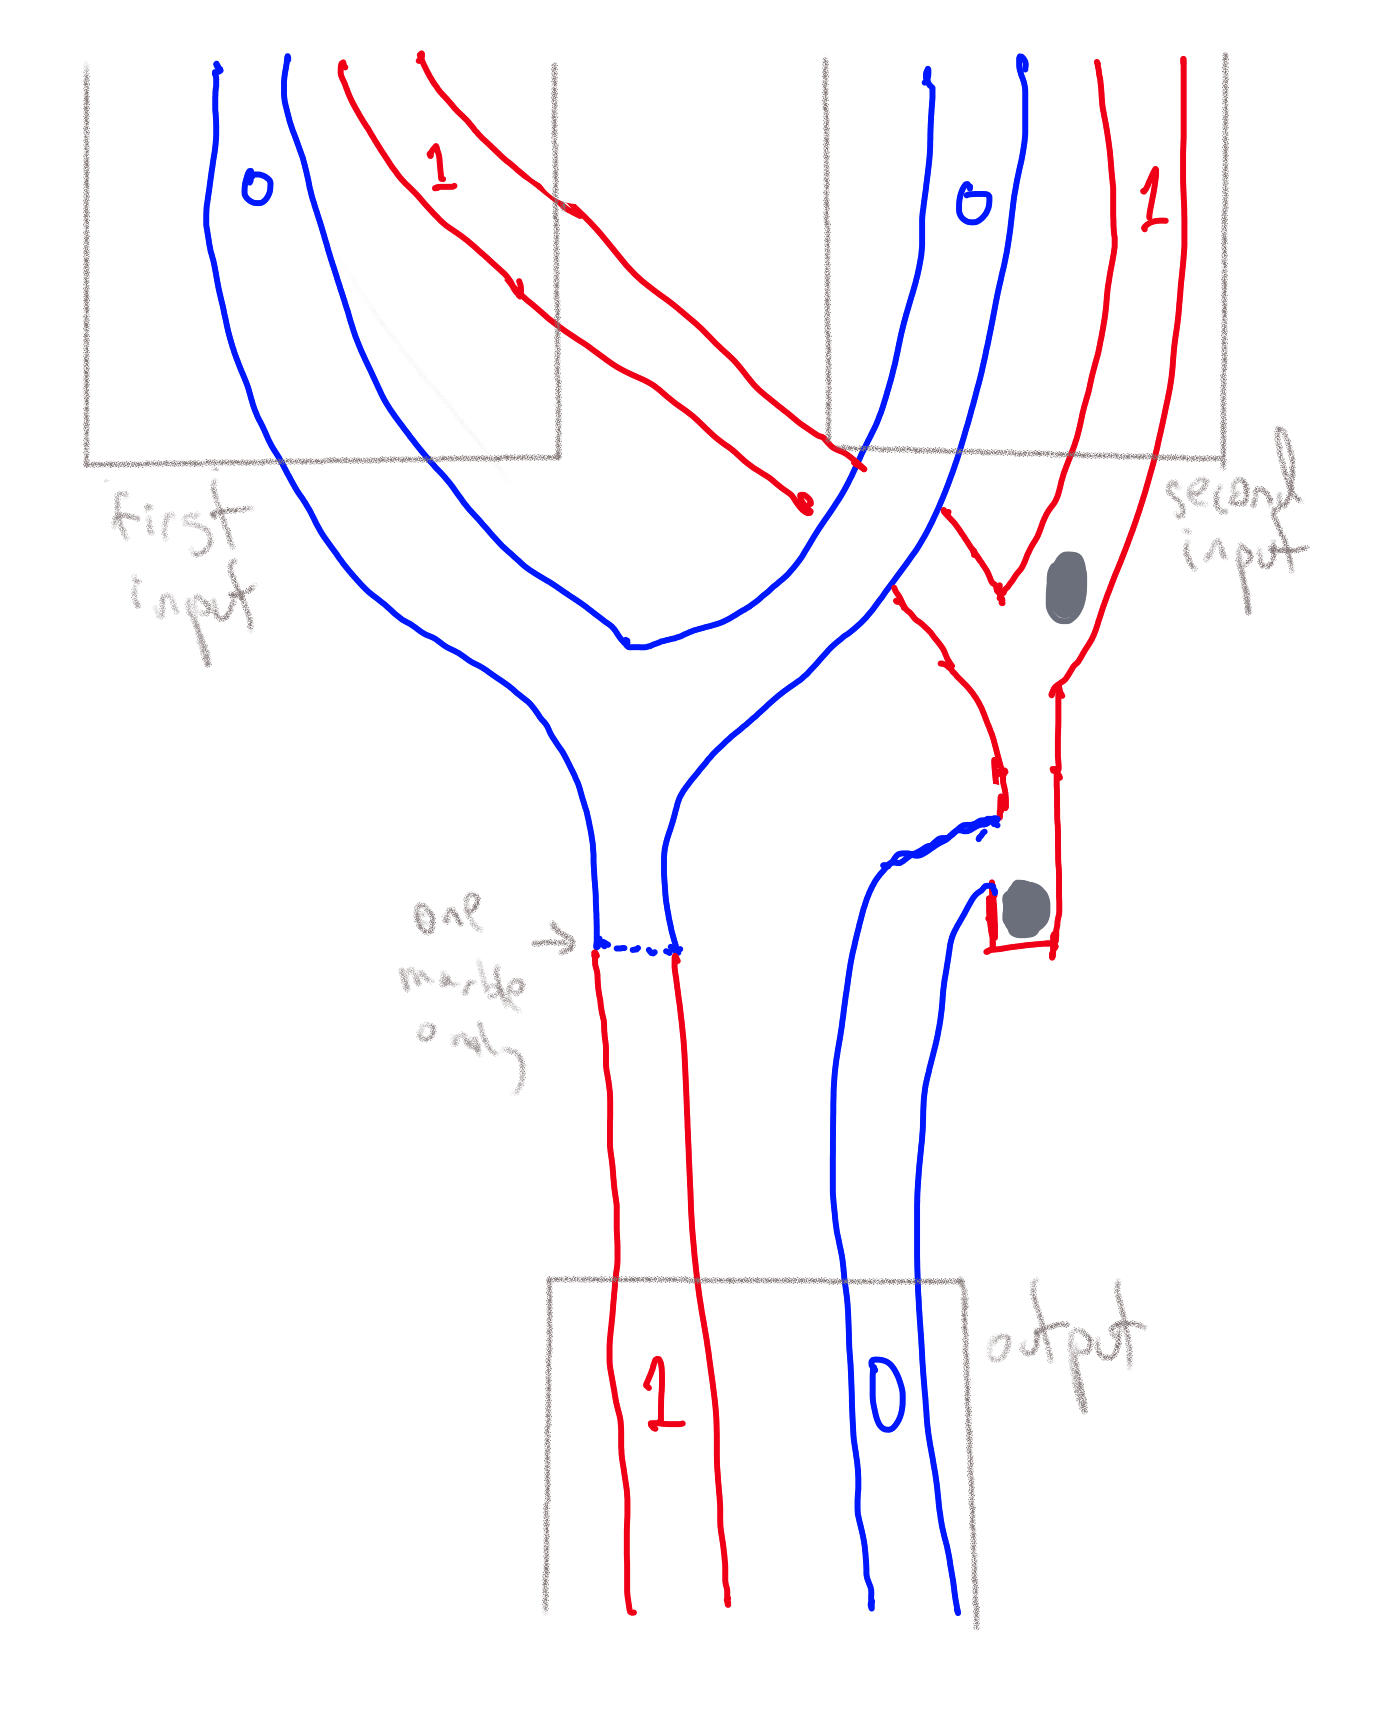
\includegraphics[width=\linewidth, height=1.5in, keepaspectratio]{../figure/marble.png}
\caption{A physical implementation of a NAND gate using marbles. Each
wire in a Boolean circuit is modeled by a pair of pipes representing the
values \(0\) and \(1\) respectively, and hence a gate has four input
pipes (two for each logical input) and two output pipes. If one of the
input pipes representing the value \(0\) has a marble in it then that
marble will flow to the output pipe representing the value \(1\). (The
dashed line represents a gadget that will ensure that at most one marble
is allowed to flow onward in the pipe.) If both the input pipes
representing the value \(1\) have marbles in them, then the first marble
will be stuck but the second one will flow onwards to the output pipe
representing the value \(0\).}
\label{marblefig}
\end{marginfigure}


\begin{marginfigure}
\centering
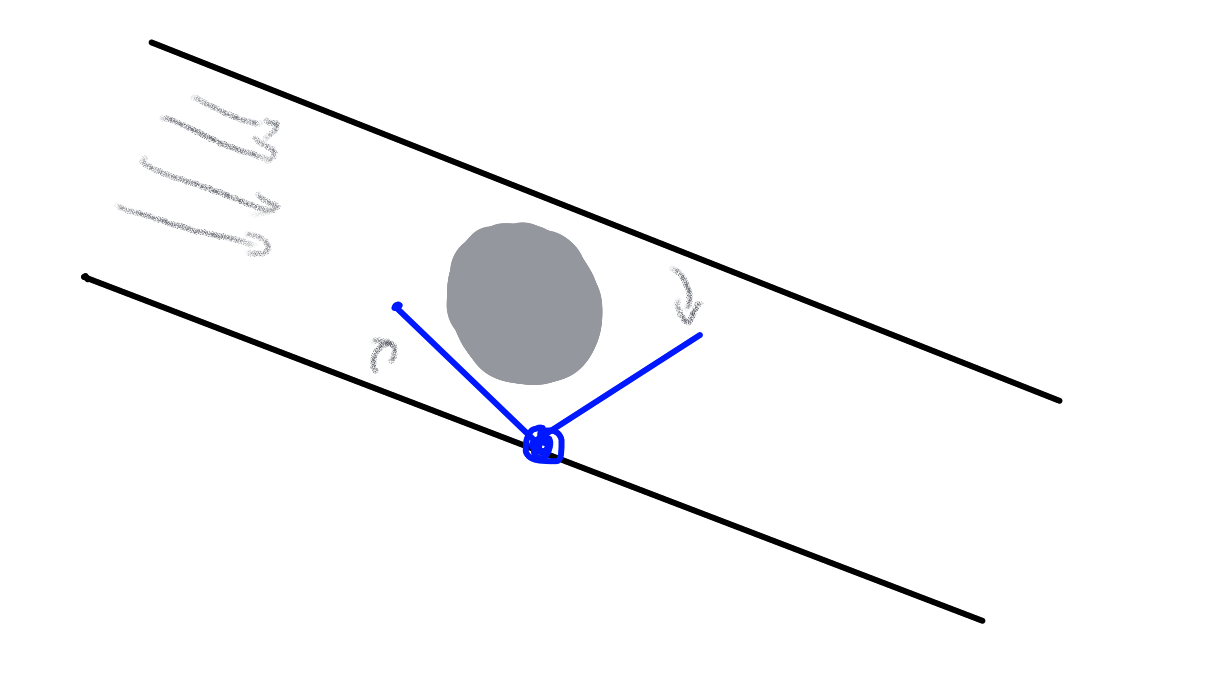
\includegraphics[width=\linewidth, height=1.5in, keepaspectratio]{../figure/gadget.png}
\caption{A ``gadget'' in a pipe that ensures that at most one marble can
pass through it. The first marble that passes causes the barrier to lift
and block new ones.}
\label{gadgetfig}
\end{marginfigure}


\begin{marginfigure}
\centering
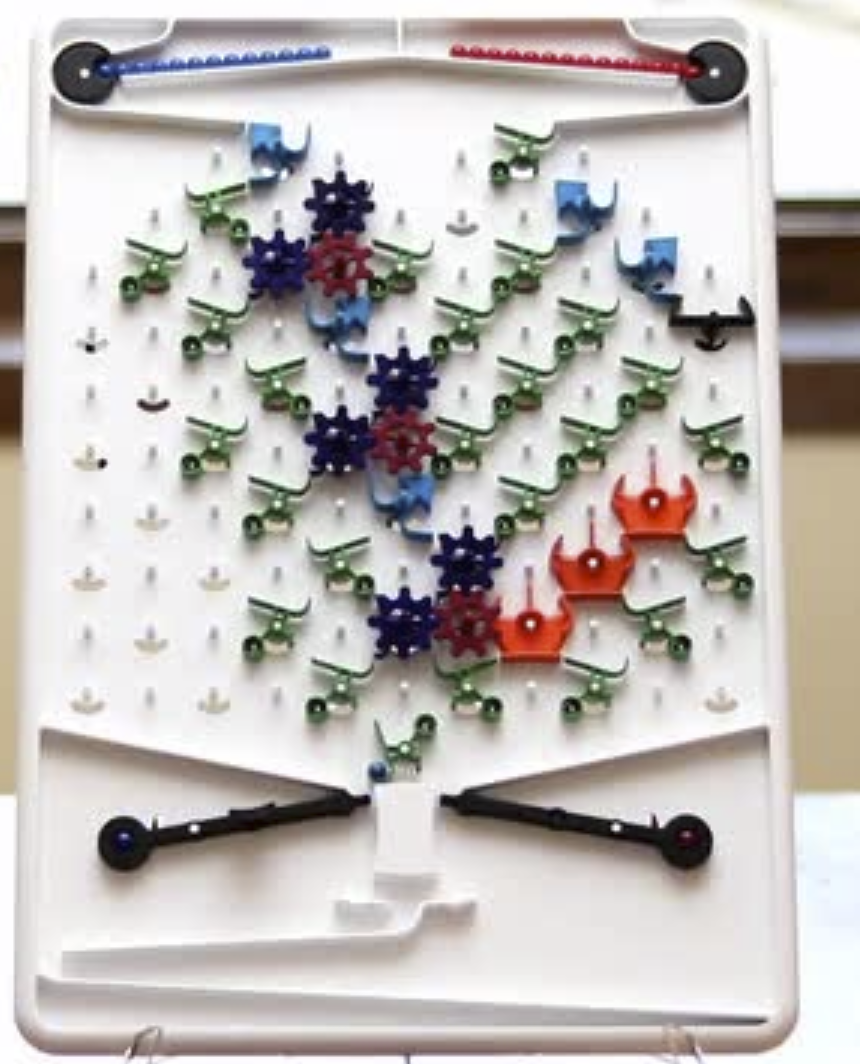
\includegraphics[width=\linewidth, height=1.5in, keepaspectratio]{../figure/turingtumble.png}
\caption{The game \href{https://www.turingtumble.com/}{``Turing
Tumble''} contains an implementation of logical gates using marbles.}
\label{turingtumblefig}
\end{marginfigure}

\section{The NAND function}\label{nandsec}

The \(\ensuremath{\mathit{NAND}}\) function is another simple function
that is extremely useful for defining computation. It is the function
mapping \(\{0,1\}^2\) to \(\{0,1\}\) defined by:

\[\ensuremath{\mathit{NAND}}(a,b) = \begin{cases} 0 & a=b=1 \\ 1 & \text{otherwise} \end{cases}\;.\]

As its name implies, \(\ensuremath{\mathit{NAND}}\) is the NOT of AND
(i.e.,
\(\ensuremath{\mathit{NAND}}(a,b)= \ensuremath{\mathit{NOT}}(\ensuremath{\mathit{AND}}(a,b))\)),
and so we can clearly compute \(\ensuremath{\mathit{NAND}}\) using
\(\ensuremath{\mathit{AND}}\) and \(\ensuremath{\mathit{NOT}}\).
Interestingly, the opposite direction holds as well:

\hypertarget{univnandonethm}{}
\begin{theorem}[NAND computes AND,OR,NOT] \label[theorem]{univnandonethm}

We can compute \(\ensuremath{\mathit{AND}}\),
\(\ensuremath{\mathit{OR}}\), and \(\ensuremath{\mathit{NOT}}\) by
composing only the \(\ensuremath{\mathit{NAND}}\) function.

\end{theorem}

\begin{proof} \label[proof]{We-start-with-the-followi}

We start with the following observation. For every \(a\in \{0,1\}\),
\(\ensuremath{\mathit{AND}}(a,a)=a\). Hence,
\(\ensuremath{\mathit{NAND}}(a,a)=\ensuremath{\mathit{NOT}}(\ensuremath{\mathit{AND}}(a,a))=\ensuremath{\mathit{NOT}}(a)\).
This means that \(\ensuremath{\mathit{NAND}}\) can compute
\(\ensuremath{\mathit{NOT}}\). By the principle of ``double negation'',
\(\ensuremath{\mathit{AND}}(a,b)=\ensuremath{\mathit{NOT}}(\ensuremath{\mathit{NOT}}(\ensuremath{\mathit{AND}}(a,b)))\),
and hence we can use \(\ensuremath{\mathit{NAND}}\) to compute
\(\ensuremath{\mathit{AND}}\) as well. Once we can compute
\(\ensuremath{\mathit{AND}}\) and \(\ensuremath{\mathit{NOT}}\), we can
compute \(\ensuremath{\mathit{OR}}\) using
\href{https://goo.gl/TH86dH}{``De Morgan's Law''}:
\(\ensuremath{\mathit{OR}}(a,b)=\ensuremath{\mathit{NOT}}(\ensuremath{\mathit{AND}}(\ensuremath{\mathit{NOT}}(a),\ensuremath{\mathit{NOT}}(b)))\)
(which can also be written as
\(a \vee b = \overline{\overline{a} \wedge \overline{b}}\)) for every
\(a,b \in \{0,1\}\).

\end{proof}

\begin{pause} \label[pause]{crefunivnandonethms-proof}

\cref{univnandonethm}'s proof is very simple, but you should make sure
that \textbf{(i)} you understand the statement of the theorem, and
\textbf{(ii)} you follow its proof. In particular, you should make sure
you understand why De Morgan's law is true.

\end{pause}

We can use \(\ensuremath{\mathit{NAND}}\) to compute many other
functions, as demonstrated in the following exercise.

\hypertarget{majbynandex}{}
\begin{solvedexercise}[Compute majority with NAND] \label[solvedexercise]{majbynandex}

Let \(\ensuremath{\mathit{MAJ}}: \{0,1\}^3 \rightarrow \{0,1\}\) be the
function that on input \(a,b,c\) outputs \(1\) iff \(a+b+c \geq 2\).
Show how to compute \(\ensuremath{\mathit{MAJ}}\) using a composition of
\(\ensuremath{\mathit{NAND}}\)'s.

\end{solvedexercise}

\begin{solution} \label[solution]{Recall-that-eqrefeqmajand}

Recall that \eqref{eqmajandornot} states that

\[
\ensuremath{\mathit{MAJ}}(x_0,x_1,x_2) = \ensuremath{\mathit{OR}}\left(\, \ensuremath{\mathit{AND}}(x_0,x_1)\;,\; \ensuremath{\mathit{OR}} \bigl( \ensuremath{\mathit{AND}}(x_1,x_2) \;,\; \ensuremath{\mathit{AND}}(x_0,x_2) \bigr) \, \right) \;. \label{eqmajandornotrestated}
\]

We can use \cref{univnandonethm} to replace all the occurrences of
\(\ensuremath{\mathit{AND}}\) and \(\ensuremath{\mathit{OR}}\) with
\(\ensuremath{\mathit{NAND}}\)'s. Specifically, we can use the
equivalence
\(\ensuremath{\mathit{AND}}(a,b)=\ensuremath{\mathit{NOT}}(\ensuremath{\mathit{NAND}}(a,b))\),
\(\ensuremath{\mathit{OR}}(a,b)=\ensuremath{\mathit{NAND}}(\ensuremath{\mathit{NOT}}(a),\ensuremath{\mathit{NOT}}(b))\),
and \(\ensuremath{\mathit{NOT}}(a)=\ensuremath{\mathit{NAND}}(a,a)\) to
replace the righthand side of \eqref{eqmajandornotrestated} with an
expression involving only \(\ensuremath{\mathit{NAND}}\), yielding that
\(\ensuremath{\mathit{MAJ}}(a,b,c)\) is equivalent to the (somewhat
unwieldy) expression

\[
\begin{gathered}
\ensuremath{\mathit{NAND}} \biggl(\, \ensuremath{\mathit{NAND}}\Bigl(\, \ensuremath{\mathit{NAND}}\bigl(\ensuremath{\mathit{NAND}}(a,b),\ensuremath{\mathit{NAND}}(a,c)\bigr), \\
\ensuremath{\mathit{NAND}}\bigl(\ensuremath{\mathit{NAND}}(a,b),\ensuremath{\mathit{NAND}}(a,c)\bigr)\, \Bigr),\\
\ensuremath{\mathit{NAND}}(b,c) \, \biggr)
\end{gathered}
\]

The same formula can also be expressed as a circuit with NAND gates, see
\cref{majnandcircfig}.

\end{solution}


\begin{marginfigure}
\centering
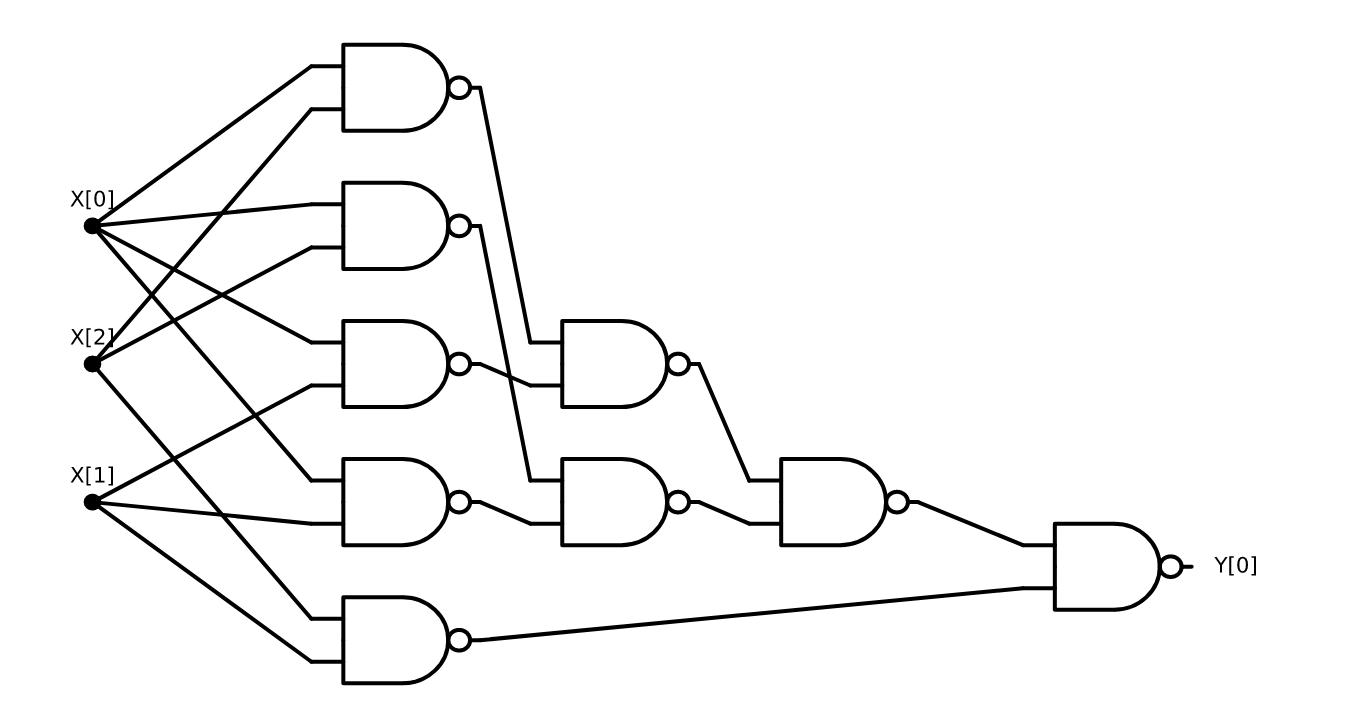
\includegraphics[width=\linewidth, height=1.5in, keepaspectratio]{../figure/majfromnand.png}
\caption{A circuit with NAND gates to compute the Majority function on
three bits}
\label{majnandcircfig}
\end{marginfigure}

\subsection{NAND Circuits}\label{NAND-Circuits}

We define \emph{NAND Circuits} as circuits in which all the gates are
NAND operations. Such a circuit again corresponds to a directed acyclic
graph (DAG) since all the gates correspond to the same function (i.e.,
NAND), we do not even need to label them, and all gates have in-degree
exactly two. Despite their simplicity, NAND circuits can be quite
powerful.

\hypertarget{xornandexample}{}
\begin{example}[$NAND$ circuit for $XOR$] \label[example]{xornandexample}

Recall the \(\ensuremath{\mathit{XOR}}\) function which maps
\(x_0,x_1 \in \{0,1\}\) to \(x_0 + x_1 \mod 2\). We have seen in
\cref{xoraonexample} that we can compute \(\ensuremath{\mathit{XOR}}\)
using \(\ensuremath{\mathit{AND}}\), \(\ensuremath{\mathit{OR}}\), and
\(\ensuremath{\mathit{NOT}}\), and so by \cref{univnandonethm} we can
compute it using only \(\ensuremath{\mathit{NAND}}\)'s. However, the
following is a direct construction of computing
\(\ensuremath{\mathit{XOR}}\) by a sequence of NAND operations:

\begin{enumerate}
\def\labelenumi{\arabic{enumi}.}
\tightlist
\item
  Let \(u = \ensuremath{\mathit{NAND}}(x_0,x_1)\).
\item
  Let \(v = \ensuremath{\mathit{NAND}}(x_0,u)\)
\item
  Let \(w = \ensuremath{\mathit{NAND}}(x_1,u)\).
\item
  The \(\ensuremath{\mathit{XOR}}\) of \(x_0\) and \(x_1\) is
  \(y_0 = \ensuremath{\mathit{NAND}}(v,w)\).
\end{enumerate}

One can verify that this algorithm does indeed compute
\(\ensuremath{\mathit{XOR}}\) by enumerating all the four choices for
\(x_0,x_1 \in \{0,1\}\). We can also represent this algorithm
graphically as a circuit, see \cref{cornandcircfig}.

\end{example}


\begin{marginfigure}
\centering
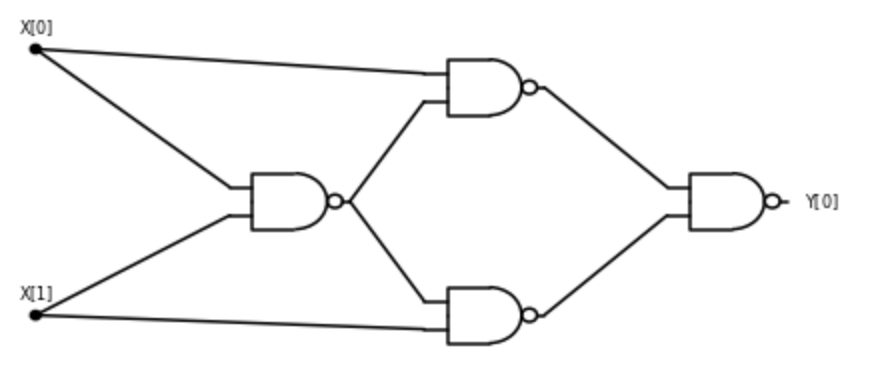
\includegraphics[width=\linewidth, height=1.5in, keepaspectratio]{../figure/nandcircxor.png}
\caption{A circuit with NAND gates to compute the XOR of two bits.}
\label{cornandcircfig}
\end{marginfigure}

In fact, we can show the following theorem:

\hypertarget{NANDuniversamthm}{}
\begin{theorem}[NAND is a universal operation] \label[theorem]{NANDuniversamthm}

For every Boolean circuit \(C\) of \(s\) gates, there exists a NAND
circuit \(C'\) of at most \(3s\) gates that computes the same function
as \(C\).

\end{theorem}

\begin{proofidea} \label[proofidea]{The-idea-of-the-proof-is-}

The idea of the proof is to just replace every
\(\ensuremath{\mathit{AND}}\), \(\ensuremath{\mathit{OR}}\) and
\(\ensuremath{\mathit{NOT}}\) gate with their NAND implementation
following the proof of \cref{univnandonethm}.

\end{proofidea}

\begin{proof}[Proof of \cref{NANDuniversamthm}] \label[proof]{If-C-is-a-Boolean-circuit}

If \(C\) is a Boolean circuit, then since, as we've seen in the proof of
\cref{univnandonethm}, for every \(a,b \in \{0,1\}\)

\begin{itemize}
\item
  \(\ensuremath{\mathit{NOT}}(a) = \ensuremath{\mathit{NAND}}(a,a)\)
\item
  \(\ensuremath{\mathit{AND}}(a,b) = \ensuremath{\mathit{NAND}}(\ensuremath{\mathit{NAND}}(a,b),\ensuremath{\mathit{NAND}}(a,b))\)
\item
  \(\ensuremath{\mathit{OR}}(a,b) = \ensuremath{\mathit{NAND}}(\ensuremath{\mathit{NAND}}(a,a),\ensuremath{\mathit{NAND}}(b,b))\)
\end{itemize}

we can replace every gate of \(C\) with at most three
\(\ensuremath{\mathit{NAND}}\) gates to obtain an equivalent circuit
\(C'\). The resulting circuit will have at most \(3s\) gates.

\end{proof}

\hypertarget{equivalencemodels}{}
\begin{bigidea} \label[bigidea]{equivalencemodels}

Two models are \emph{equivalent in power} if they can be used to compute
the same set of functions.

\end{bigidea}

\subsection{More examples of NAND circuits
(optional)}\label{More-examples-of-NAND-cir}

Here are some more sophisticated examples of NAND circuits:

\paragraph{Incrementing integers.} Consider the task of computing, given
as input a string \(x\in \{0,1\}^n\) that represents a natural number
\(X\in \N\), the representation of \(X+1\). That is, we want to compute
the function
\(\ensuremath{\mathit{INC}}_n:\{0,1\}^n \rightarrow \{0,1\}^{n+1}\) such
that for every \(x_0,\ldots,x_{n-1}\),
\(\ensuremath{\mathit{INC}}_n(x)=y\) which satisfies
\(\sum_{i=0}^n y_i 2^i = \left( \sum_{i=0}^{n-1} x_i 2^i \right)+1\).
(For simplicity of notation, in this example we use the representation
where the least significant digit is first rather than last.)

The increment operation can be very informally described as follows:
\emph{``Add \(1\) to the least significant bit and propagate the
carry''}. A little more precisely, in the case of the binary
representation, to obtain the increment of \(x\), we scan \(x\) from the
least significant bit onwards, and flip all \(1\)'s to \(0\)'s until we
encounter a bit equal to \(0\), in which case we flip it to \(1\) and
stop.

Thus we can compute the increment of \(x_0,\ldots,x_{n-1}\) by doing the
following:

\begin{algorithm}[Compute Increment Function]
\label[algorithm]{incrementalg} ~ \\ \noindent
\begin{algorithmic}[1]
\INPUT  $x_0,x_1,\ldots,x_{n-1}$ representing the number $\sum_{i=0}^{n-1} x_i\cdot 2^i$ \COMMENT{ we use LSB-first representation}
\OUTPUT $y \in \{0,1\}^{n+1}$ such that $\sum_{i=0}^n y_i \cdot 2^i =  \sum_{i=0}^{n-1} x_i\cdot 2^i + 1$
\STATE Let $c_0 \leftarrow 1$ \COMMENT{ we pretend we have a "carry" of $1$ initially}
\FOR{$i=0,\ldots, n-1$}
\STATE Let $y_i \leftarrow XOR(x_i,c_i)$.
\IF{$c_i=x_i=1$}
\STATE $c_{i+1}=1$
\ELSE
\STATE $c_{i+1}=0$
\ENDIF
\ENDFOR
\STATE Let $y_n \leftarrow c_n$.
\end{algorithmic}
\end{algorithm}

\cref{incrementalg} describes precisely how to compute the increment
operation, and can be easily transformed into \emph{Python} code that
performs the same computation, but it does not seem to directly yield a
NAND circuit to compute this. However, we can transform this algorithm
line by line to a NAND circuit. For example, since for every \(a\),
\(\ensuremath{\mathit{NAND}}(a,\ensuremath{\mathit{NOT}}(a))=1\), we can
replace the initial statement \(c_0=1\) with
\(c_0 = \ensuremath{\mathit{NAND}}(x_0,\ensuremath{\mathit{NAND}}(x_0,x_0))\).
We already know how to compute \(\ensuremath{\mathit{XOR}}\) using NAND
and so we can use this to implement the operation
\(y_i \leftarrow \ensuremath{\mathit{XOR}}(x_i,c_i)\). Similarly, we can
write the ``if'' statement as saying
\(c_{i+1} \leftarrow \ensuremath{\mathit{AND}}(c_i,x_i)\), or in other
words
\(c_{i+1} \leftarrow \ensuremath{\mathit{NAND}}(\ensuremath{\mathit{NAND}}(c_i,x_i),\ensuremath{\mathit{NAND}}(c_i,x_i))\).
Finally, the assignment \(y_n = c_n\) can be written as
\(y_n = \ensuremath{\mathit{NAND}}(\ensuremath{\mathit{NAND}}(c_n,c_n),\ensuremath{\mathit{NAND}}(c_n,c_n))\).
Combining these observations yields for every \(n\in \N\), a
\(\ensuremath{\mathit{NAND}}\) circuit to compute
\(\ensuremath{\mathit{INC}}_n\). For example,
\cref{nandincrememntcircfig} shows what this circuit looks like for
\(n=4\).


\begin{marginfigure}
\centering
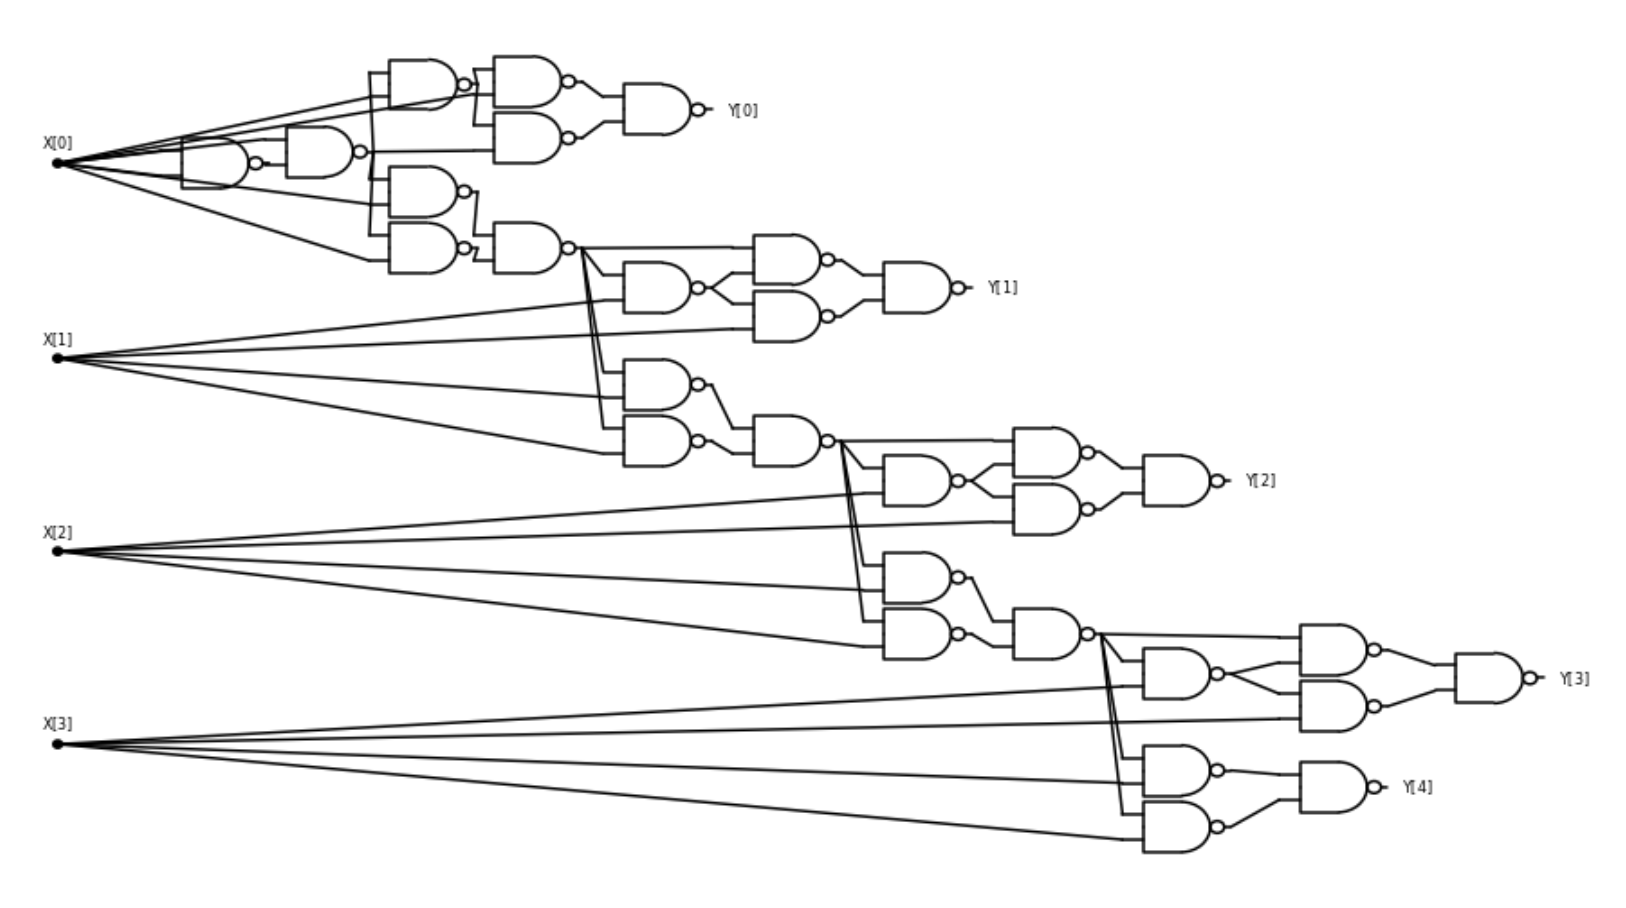
\includegraphics[width=\linewidth, height=1.5in, keepaspectratio]{../figure/incrementfromnand.png}
\caption{NAND circuit with computing the \emph{increment} function on
\(4\) bits.}
\label{nandincrememntcircfig}
\end{marginfigure}

\paragraph{From increment to addition.} Once we have the increment
operation, we can certainly compute addition by repeatedly incrementing
(i.e., compute \(x+y\) by performing \(\ensuremath{\mathit{INC}}(x)\)
\(y\) times). However, that would be quite inefficient and unnecessary.
With the same idea of keeping track of carries we can implement the
``grade-school'' addition algorithm and compute the function
\(\ensuremath{\mathit{ADD}}_n:\{0,1\}^{2n} \rightarrow \{0,1\}^{n+1}\)
that on input \(x\in \{0,1\}^{2n}\) outputs the binary representation of
the sum of the numbers represented by \(x_0,\ldots,x_{n-1}\) and
\(x_{n+1},\ldots,x_n\):

\begin{algorithm}[Addition using NAND]
\label[algorithm]{additionfromnand} ~ \\ \noindent
\begin{algorithmic}[1]
\INPUT  $u \in \{0,1\}^n$, $v\in \{0,1\}^n$ representing numbers in LSB-first binary representation.
\OUTPUT  LSB-first binary representation of $x+y$.
\STATE Let $c_0 \leftarrow 0$
\FOR{$i=0,\ldots,n-1$}
    \STATE Let $y_i \leftarrow u_i + v_i \mod 2$
    \IF{$u_i + v_i + c_i \geq 2$}
    \STATE $c_{i+1}\leftarrow 1$
    \ELSE
    \STATE $c_{i+1} \leftarrow 0$
    \ENDIF
\ENDFOR
\STATE Let $y_n \leftarrow c_n$
\end{algorithmic}
\end{algorithm}

Once again, \cref{additionfromnand} can be translated into a NAND
circuit. The crucial observation is that the ``if/then'' statement
simply corresponds to
\(c_{i+1} \leftarrow \ensuremath{\mathit{MAJ}}_3(u_i,v_i,v_i)\) and we
have seen in \cref{majbynandex} that the function
\(\ensuremath{\mathit{MAJ}}_3:\{0,1\}^3 \rightarrow \{0,1\}\) can be
computed using \(\ensuremath{\mathit{NAND}}\)s.

\subsection{The NAND-CIRC Programming language}\label{nandcircsec}

Just like we did for Boolean circuits, we can define a
programming-language analog of NAND circuits. It is even simpler than
the AON-CIRC language since we only have a single operation. We define
the \emph{NAND-CIRC Programming Language} to be a programming language
where every line has the following form:

\begin{code}
foo = NAND(bar,blah)
\end{code}

where \texttt{foo}, \texttt{bar} and \texttt{blah} are variable
identifiers.

\hypertarget{NANDprogramexample}{}
\begin{example}[Our first NAND-CIRC program] \label[example]{NANDprogramexample}

Here is an example of a NAND-CIRC program:

\begin{code}
u = NAND(X[0],X[1])
v = NAND(X[0],u)
w = NAND(X[1],u)
Y[0] = NAND(v,w)
\end{code}

\end{example}

\begin{pause} \label[pause]{Do-you-know-what-function}

Do you know what function this program computes? Hint: you have seen it
before.

\end{pause}

Formally, just like we did in \cref{AONcircdef} for AON-CIRC, we can
define the notion of computation by a NAND-CIRC program in the natural
way:

\hypertarget{NANDcomp}{}
\begin{definition}[Computing by a NAND-CIRC program] \label[definition]{NANDcomp}

Let \(f:\{0,1\}^n \rightarrow \{0,1\}^m\) be some function, and let
\(P\) be a NAND-CIRC program. We say that \(P\) \emph{computes} the
function \(f\) if:

\begin{enumerate}
\def\labelenumi{\arabic{enumi}.}
\item
  \(P\) has \(n\) input variables
  \texttt{X[}\(0\)\texttt{]}\(,\ldots,\)\texttt{X[}\(n-1\)\texttt{]} and
  \(m\) output variables
  \texttt{Y[}\(0\)\texttt{]},\(\ldots\),\texttt{Y[}\(m-1\)\texttt{]}.
\item
  For every \(x\in \{0,1\}^n\), if we execute \(P\) when we assign to
  \texttt{X[}\(0\)\texttt{]}\(,\ldots,\)\texttt{X[}\(n-1\)\texttt{]} the
  values \(x_0,\ldots,x_{n-1}\), then at the end of the execution, the
  output variables
  \texttt{Y[}\(0\)\texttt{]},\(\ldots\),\texttt{Y[}\(m-1\)\texttt{]}
  have the values \(y_0,\ldots,y_{m-1}\) where \(y=f(x)\).
\end{enumerate}

\end{definition}

As before we can show that NAND circuits are equivalent to NAND-CIRC
programs (see \cref{progandcircfig}):

\hypertarget{NANDcircslequivthm}{}
\begin{theorem}[NAND circuits and straight-line program equivalence] \label[theorem]{NANDcircslequivthm}

For every \(f:\{0,1\}^n \rightarrow \{0,1\}^m\) and \(s \geq m\), \(f\)
is computable by a NAND-CIRC program of \(s\) lines if and only if \(f\)
is computable by a NAND circuit of \(s\) gates.

\end{theorem}


\begin{marginfigure}
\centering
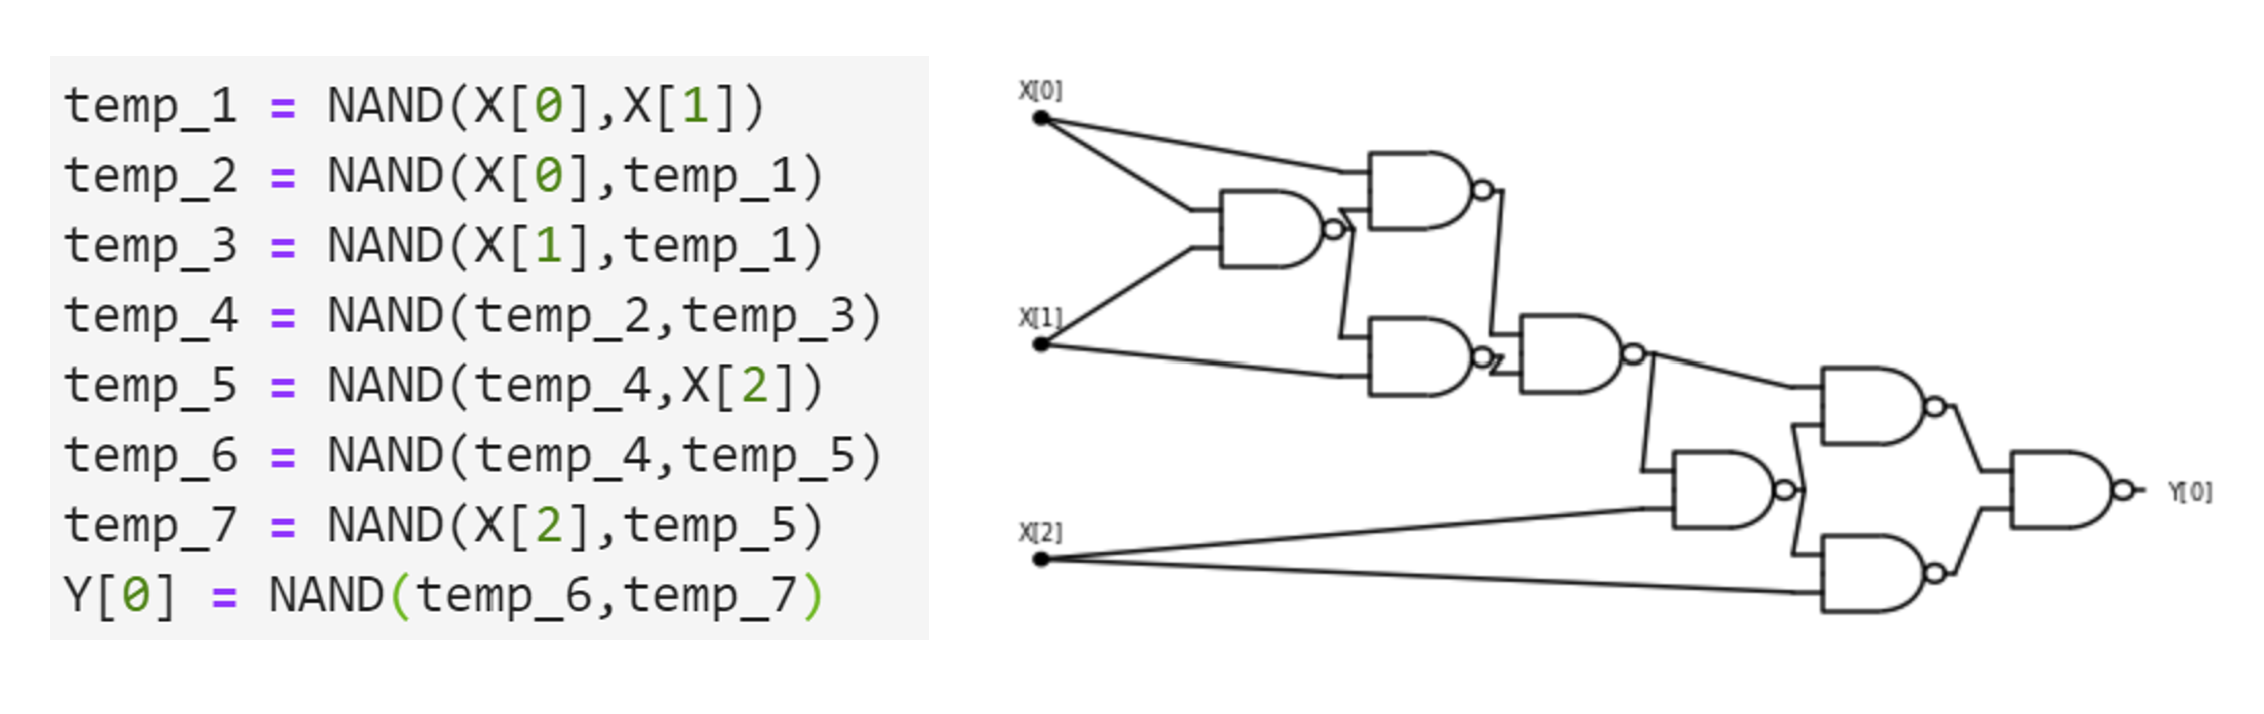
\includegraphics[width=\linewidth, height=1.5in, keepaspectratio]{../figure/nandcircuitequiv.png}
\caption{A NAND program and the corresponding circuit. Note how every
line in the program corresponds to a gate in the circuit.}
\label{progandcircfig}
\end{marginfigure}

We omit the proof of \cref{NANDcircslequivthm} since it follows along
exactly the same lines as the equivalence of Boolean circuits and
AON-CIRC program (\cref{slcircuitequivthm}). Given
\cref{NANDcircslequivthm} and \cref{NANDuniversamthm}, we know that we
can translate every \(s\)-line AON-CIRC program \(P\) into an equivalent
NAND-CIRC program of at most \(3s\) lines. In fact, this translation can
be easily done by replacing every line of the form
\texttt{foo = AND(bar,blah)}, \texttt{foo = OR(bar,blah)} or
\texttt{foo = NOT(bar)} with the equivalent 1-3 lines that use the
\texttt{NAND} operation. Our
\href{https://github.com/boazbk/tcscode}{GitHub repository} contains a
``proof by code'': a simple Python program \texttt{AON2NAND} that
transforms an AON-CIRC into an equivalent NAND-CIRC program.

\hypertarget{NANDturingcompleteness}{}
\begin{remark}[Is the NAND-CIRC programming language Turing Complete? (optional note)] \label[remark]{NANDturingcompleteness}

You might have heard of a term called ``Turing Complete'' that is
sometimes used to describe programming languages. (If you haven't, feel
free to ignore the rest of this remark: we define this term precisely in
\cref{chapequivalentmodels}.) If so, you might wonder if the NAND-CIRC
programming language has this property. The answer is \textbf{no}, or
perhaps more accurately, the term ``Turing Completeness'' is not really
applicable for the NAND-CIRC programming language. The reason is that,
by design, the NAND-CIRC programming language can only compute
\emph{finite} functions \(F:\{0,1\}^n \rightarrow \{0,1\}^m\) that take
a fixed number of input bits and produce a fixed number of outputs bits.
The term ``Turing Complete'' is only applicable to programming languages
for \emph{infinite} functions that can take inputs of arbitrary length.
We will come back to this distinction later on in this book.

\end{remark}

\section{Equivalence of all these
models}\label{Equivalence-of-all-these-}

If we put together \cref{slcircuitequivthm}, \cref{NANDuniversamthm},
and \cref{NANDcircslequivthm}, we obtain the following result:

\hypertarget{equivalencemodelsthm}{}
\begin{theorem}[Equivalence between models of finite computation] \label[theorem]{equivalencemodelsthm}

For every sufficiently large \(s,n,m\) and
\(f:\{0,1\}^n \rightarrow \{0,1\}^m\), the following conditions are all
equivalent to one another:

\begin{itemize}
\item
  \(f\) can be computed by a Boolean circuit (with \(\wedge,\vee,\neg\)
  gates) of at most \(O(s)\) gates.
\item
  \(f\) can be computed by an AON-CIRC straight-line program of at most
  \(O(s)\) lines.
\item
  \(f\) can be computed by a NAND circuit of at most \(O(s)\) gates.
\item
  \(f\) can be computed by a NAND-CIRC straight-line program of at most
  \(O(s)\) lines.
\end{itemize}

\end{theorem}

By ``\(O(s)\)'' we mean that the bound is at most \(c\cdot s\) where
\(c\) is a constant that is independent of \(n\). For example, if \(f\)
can be computed by a Boolean circuit of \(s\) gates, then it can be
computed by a NAND-CIRC program of at most \(3s\) lines, and if \(f\)
can be computed by a NAND circuit of \(s\) gates, then it can be
computed by an AON-CIRC program of at most \(2s\) lines.

\begin{proofidea} \label[proofidea]{We-omit-the-formal-proof-}

We omit the formal proof, which is obtained by combining
\cref{slcircuitequivthm}, \cref{NANDuniversamthm}, and
\cref{NANDcircslequivthm}. The key observation is that the results we
have seen allow us to translate a program/circuit that computes \(f\) in
one of the above models into a program/circuit that computes \(f\) in
another model by increasing the lines/gates by at most a constant factor
(in fact this constant factor is at most \(3\)).

\end{proofidea}

\cref{slcircuitequivthm} is a special case of a more general result. We
can consider even more general models of computation, where instead of
AND/OR/NOT or NAND, we use other operations (see \cref{othergatessec}
below). It turns out that Boolean circuits are equivalent in power to
such models as well. The fact that all these different ways to define
computation lead to equivalent models shows that we are ``on the right
track''. It justifies the seemingly arbitrary choices that we've made of
using AND/OR/NOT or NAND as our basic operations, since these choices do
not affect the power of our computational model. Equivalence results
such as \cref{equivalencemodelsthm} mean that we can easily translate
between Boolean circuits, NAND circuits, NAND-CIRC programs and the
like. We will use this ability later on in this book, often shifting to
the most convenient formulation without making a big deal about it.
Hence we will not worry too much about the distinction between, for
example, Boolean circuits and NAND-CIRC programs.

In contrast, we will continue to take special care to distinguish
between \emph{circuits/programs} and \emph{functions} (recall
\cref{functionprogramidea}). A function corresponds to a
\emph{specification} of a computational task, and it is a fundamentally
different object than a program or a circuit, which corresponds to the
\emph{implementation} of the task.

\subsection{Circuits with other gate sets}\label{othergatessec}

There is nothing special about AND/OR/NOT or NAND. For every set of
functions \(\mathcal{G} = \{ G_0,\ldots,G_{k-1} \}\), we can define a
notion of circuits that use elements of \(\mathcal{G}\) as gates, and a
notion of a ``\(\mathcal{G}\) programming language'' where every line
involves assigning to a variable \texttt{foo} the result of applying
some \(G_i \in \mathcal{G}\) to previously defined or input variables.
Specifically, we can make the following definition:

\hypertarget{genstraight-lineprogs}{}
\begin{definition}[General straight-line programs] \label[definition]{genstraight-lineprogs}

Let \(\mathcal{F} = \{ f_0,\ldots, f_{t-1} \}\) be a finite collection
of Boolean functions, such that
\(f_i:\{0,1\}^{k_i} \rightarrow \{0,1\}\) for some \(k_i \in \N\). An
\emph{\(\mathcal{F}\) program} is a sequence of lines, each of which
assigns to some variable the result of applying some
\(f_i \in \mathcal{F}\) to \(k_i\) other variables. As above, we use
\texttt{X[}\(i\)\texttt{]} and \texttt{Y[}\(j\)\texttt{]} to denote the
input and output variables.

We say that \(\mathcal{F}\) is a \emph{universal set of operations}
(also known as a universal gate set) if there exists a \(\mathcal{F}\)
program to compute the function \(\ensuremath{\mathit{NAND}}\).

\end{definition}

AON-CIRC programs correspond to
\(\{AND,\ensuremath{\mathit{OR}},\ensuremath{\mathit{NOT}}\}\) programs,
NAND-CIRC programs corresponds to \(\mathcal{F}\) programs for the set
\(\mathcal{F}\) that only contains the \(\ensuremath{\mathit{NAND}}\)
function, but we can also define
\(\{ \ensuremath{\mathit{IF}}, \ensuremath{\mathit{ZERO}}, \ensuremath{\mathit{ONE}}\}\)
programs (see below), or use any other set.

We can also define \emph{\(\mathcal{F}\) circuits}, which will be
directed graphs in which each \emph{gate} corresponds to applying a
function \(f_i \in \mathcal{F}\), and will each have \(k_i\) incoming
wires and a single outgoing wire. (If the function \(f_i\) is not
\emph{symmetric}, in the sense that the order of its input matters then
we need to label each wire entering a gate as to which parameter of the
function it corresponds to.) As in \cref{slcircuitequivthm}, we can show
that \(\mathcal{F}\) circuits and \(\mathcal{F}\) programs are
equivalent. We have seen that for
\(\mathcal{F} = \{ \ensuremath{\mathit{AND}},\ensuremath{\mathit{OR}}, \ensuremath{\mathit{NOT}}\}\),
the resulting circuits/programs are equivalent in power to the NAND-CIRC
programming language, as we can compute \(\ensuremath{\mathit{NAND}}\)
using
\(\ensuremath{\mathit{AND}}\)/\(\ensuremath{\mathit{OR}}\)/\(\ensuremath{\mathit{NOT}}\)
and vice versa. This turns out to be a special case of a general
phenomena--- the \emph{universality} of \(\ensuremath{\mathit{NAND}}\)
and other gate sets --- that we will explore more in depth later in this
book.

\hypertarget{IZOcircuits}{}
\begin{example}[IF,ZERO,ONE circuits] \label[example]{IZOcircuits}

Let
\(\mathcal{F} = \{ \ensuremath{\mathit{IF}} , \ensuremath{\mathit{ZERO}}, \ensuremath{\mathit{ONE}} \}\)
where \(\ensuremath{\mathit{ZERO}}:\{0,1\} \rightarrow \{0\}\) and
\(\ensuremath{\mathit{ONE}}:\{0,1\} \rightarrow \{1\}\) are the constant
zero and one functions,\footnote{One can also define these functions as
  taking a length zero input. This makes no difference for the
  computational power of the model.} and
\(\ensuremath{\mathit{IF}}:\{0,1\}^3 \rightarrow \{0,1\}\) is the
function that on input \((a,b,c)\) outputs \(b\) if \(a=1\) and \(c\)
otherwise. Then \(\mathcal{F}\) is universal.

Indeed, we can demonstrate that
\(\{ \ensuremath{\mathit{IF}}, \ensuremath{\mathit{ZERO}} , \ensuremath{\mathit{ONE}} \}\)
is universal using the following formula for
\(\ensuremath{\mathit{NAND}}\):

\[
\ensuremath{\mathit{NAND}}(a,b) = \ensuremath{\mathit{IF}}(a,\ensuremath{\mathit{IF}}(b,\ensuremath{\mathit{ZERO}},\ensuremath{\mathit{ONE}}),\ensuremath{\mathit{ONE}}) \;.
\]

\end{example}

There are also some sets \(\mathcal{F}\) that are more restricted in
power. For example it can be shown that if we use only AND or OR gates
(without NOT) then we do \emph{not} get an equivalent model of
computation. The exercises cover several examples of universal and
non-universal gate sets.

\subsection{Specification vs.~implementation
(again)}\label{specvsimplrem}


\begin{figure}
\centering
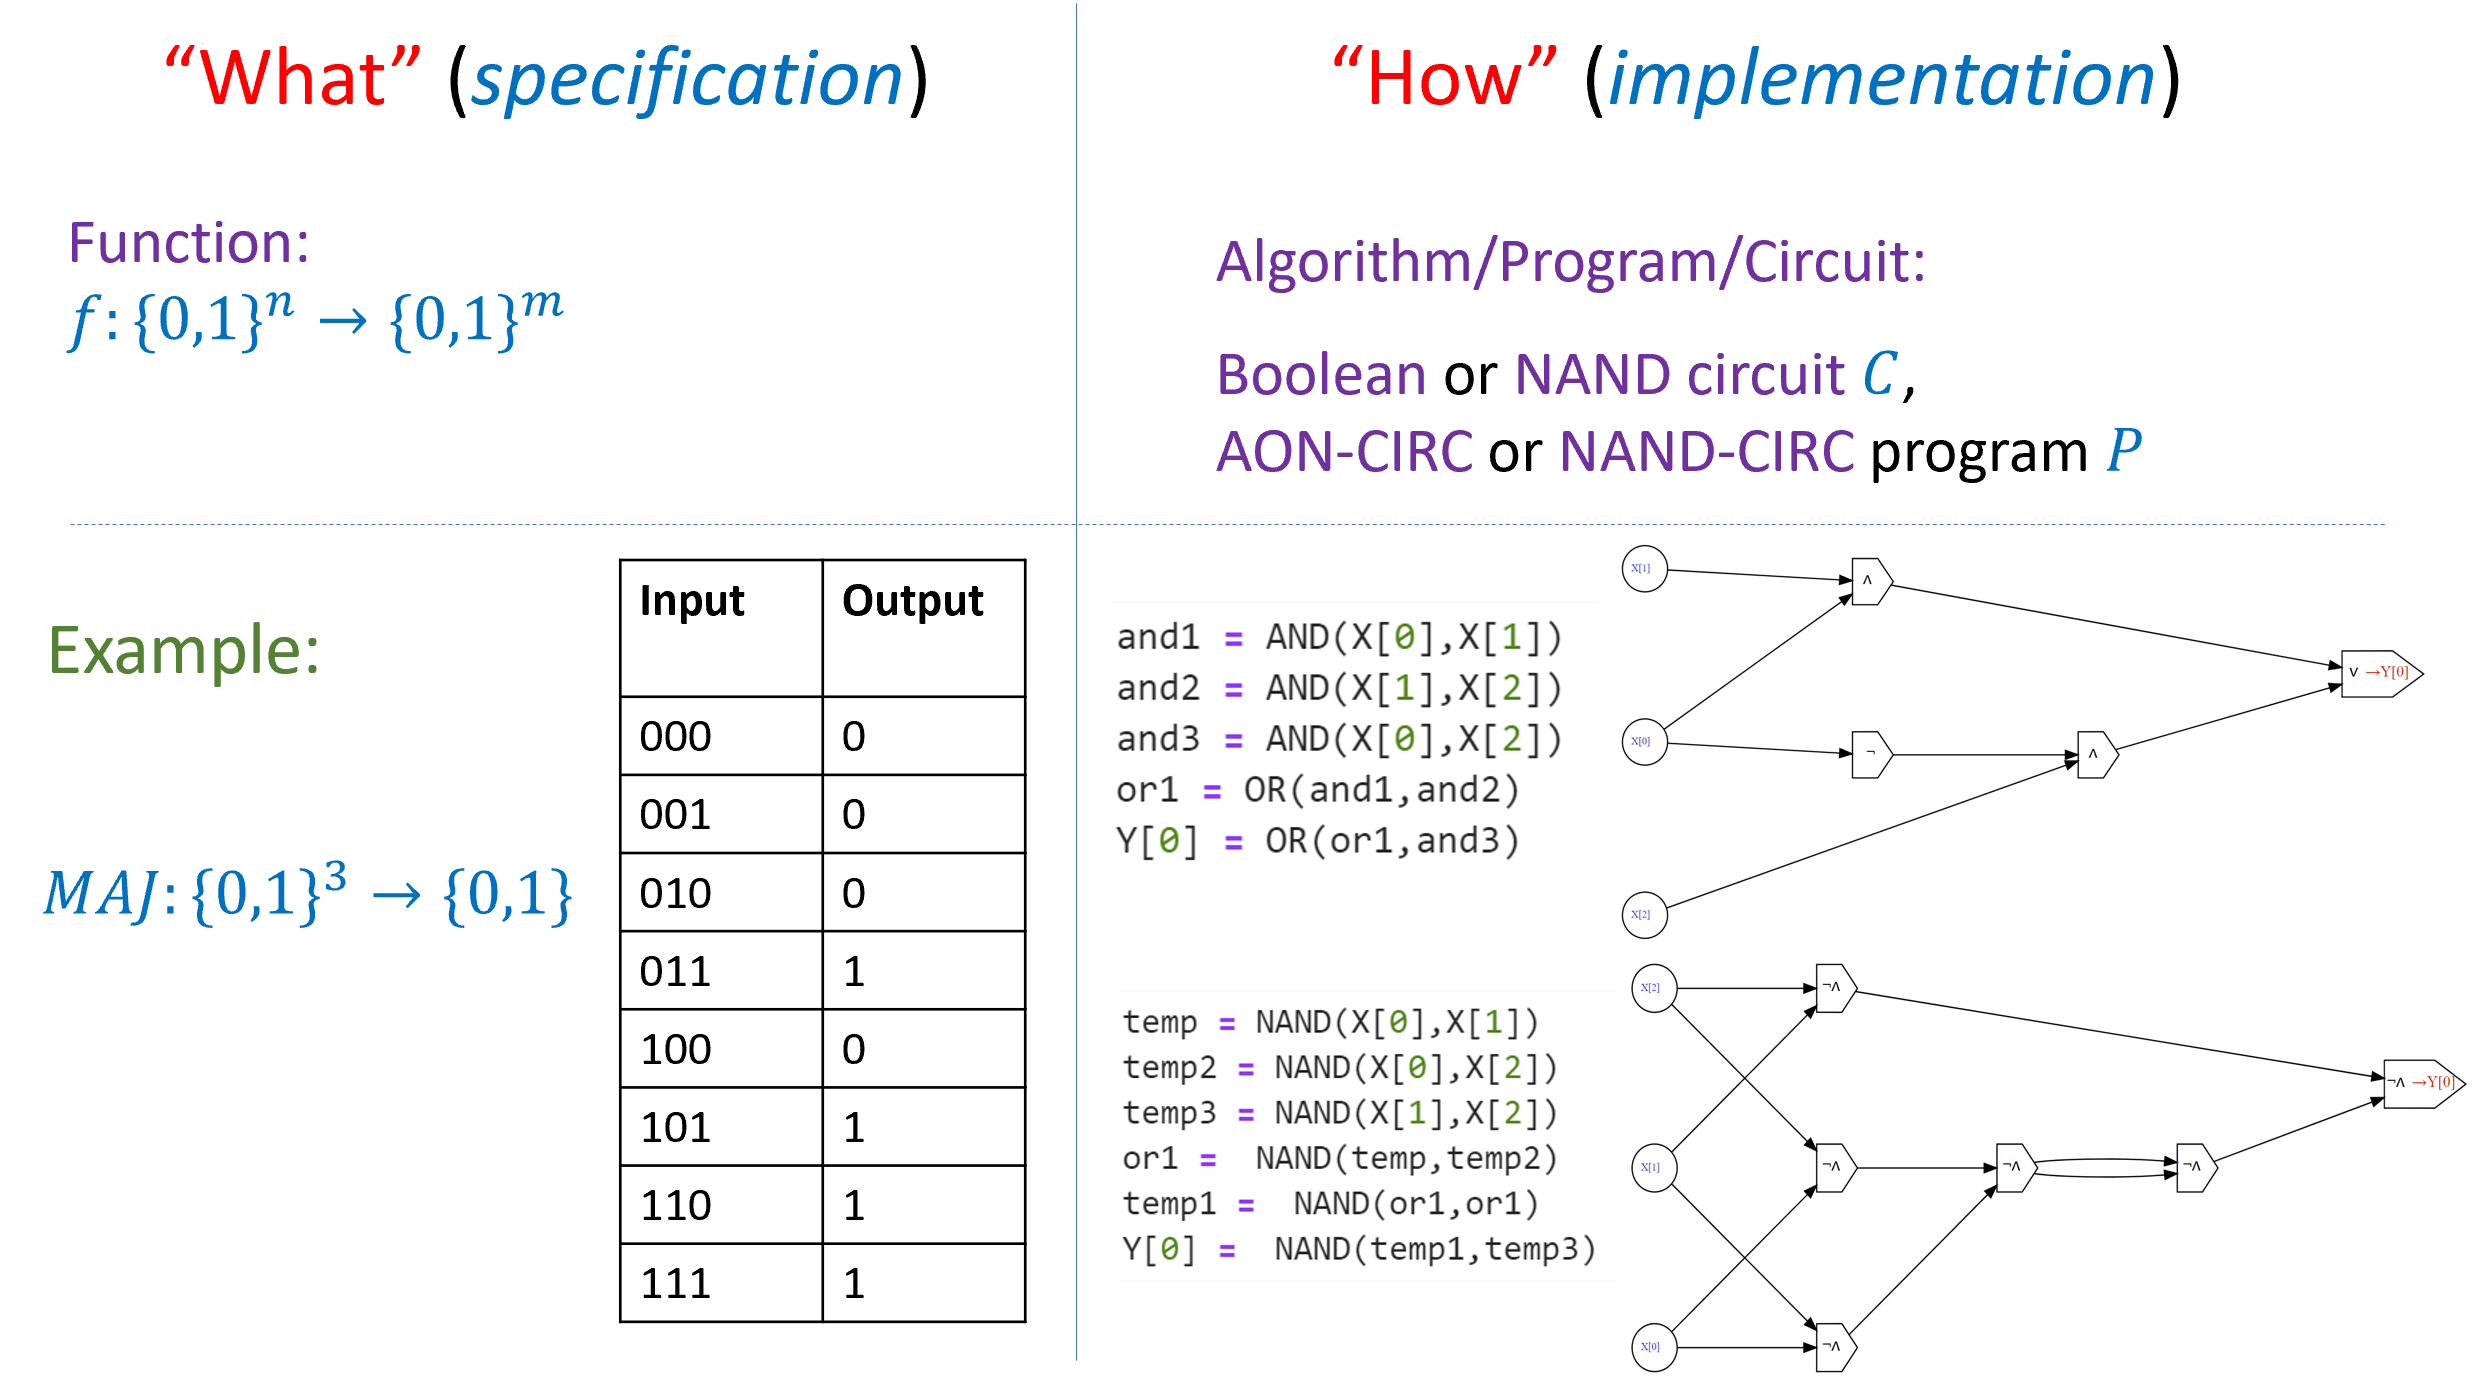
\includegraphics[width=\textwidth, height=0.25\paperheight, keepaspectratio]{../figure/specvsimpl.png}
\caption{It is crucial to distinguish between the \emph{specification}
of a computational task, namely \emph{what} is the function that is to
be computed and the \emph{implementation} of it, namely the algorithm,
program, or circuit that contains the instructions defining \emph{how}
to map an input to an output. The same function could be computed in
many different ways.}
\label{specvsimplfig}
\end{figure}

As we discussed in \cref{secimplvsspec}, one of the most important
distinctions in this book is that of \emph{specification} versus
\emph{implementation} or separating ``what'' from ``how'' (see
\cref{specvsimplfig}). A \emph{function} corresponds to the
\emph{specification} of a computational task, that is \emph{what} output
should be produced for every particular input. A \emph{program} (or
circuit, or any other way to specify \emph{algorithms}) corresponds to
the \emph{implementation} of \emph{how} to compute the desired output
from the input. That is, a program is a set of instructions how to
compute the output from the input. Even within the same computational
model there can be many different ways to compute the same function. For
example, there is more than one NAND-CIRC program that computes the
majority function, more than one Boolean circuit to compute the addition
function, and so on and so forth.

Confusing specification and implementation (or equivalently
\emph{functions} and \emph{programs}) is a common mistake, and one that
is unfortunately encouraged by the common programming-language
terminology of referring to parts of programs as ``functions''. However,
in both the theory and practice of computer science, it is important to
maintain this distinction, and it is particularly important for us in
this book.

\begin{recap} \label[recap]{An-algorithm-is-a-recipe-}

\begin{itemize}
\tightlist
\item
  An \emph{algorithm} is a recipe for performing a computation as a
  sequence of ``elementary'' or ``simple'' operations.
\item
  One candidate definition for ``elementary'' operations is the set
  \(\ensuremath{\mathit{AND}}\), \(\ensuremath{\mathit{OR}}\) and
  \(\ensuremath{\mathit{NOT}}\).
\item
  Another candidate definition for an ``elementary'' operation is the
  \(\ensuremath{\mathit{NAND}}\) operation. It is an operation that is
  easily implementable in the physical world in a variety of methods
  including by electronic transistors.
\item
  We can use \(\ensuremath{\mathit{NAND}}\) to compute many other
  functions, including majority, increment, and others.
\item
  There are other equivalent choices, including the sets
  \(\{AND,\ensuremath{\mathit{OR}},\ensuremath{\mathit{NOT}}\}\) and
  \(\{ \ensuremath{\mathit{IF}}, \ensuremath{\mathit{ZERO}}, \ensuremath{\mathit{ONE}} \}\).
\item
  We can formally define the notion of a function
  \(F:\{0,1\}^n \rightarrow \{0,1\}^m\) being computable using the
  \emph{NAND-CIRC Programming language}.
\item
  For every set of basic operations, the notions of being computable by
  a circuit and being computable by a straight-line program are
  equivalent.
\end{itemize}

\end{recap}

\section{Exercises}\label{Exercises}

\hypertarget{comparenumbersex}{}
\begin{exercise}[Compare $4$ bit numbers] \label[exercise]{comparenumbersex}

Give a Boolean circuit (with AND/OR/NOT gates) that computes the
function \(\ensuremath{\mathit{CMP}}_8:\{0,1\}^8 \rightarrow \{0,1\}\)
such that
\(\ensuremath{\mathit{CMP}}_8(a_0,a_1,a_2,a_3,b_0,b_1,b_2,b_3)=1\) if
and only if the number represented by \(a_0a_1a_2a_3\) is larger than
the number represented by \(b_0b_1b_2b_3\).

\end{exercise}

\hypertarget{compareasymnumbersex}{}
\begin{exercise}[Compare $n$ bit numbers] \label[exercise]{compareasymnumbersex}

Prove that there exists a constant \(c\) such that for every \(n\) there
is a Boolean circuit (with AND/OR/NOT gates) \(C\) of at most
\(c\cdot n\) gates that computes the function
\(\ensuremath{\mathit{CMP}}_{2n}:\{0,1\}^{2n} \rightarrow \{0,1\}\) such
that
\(\ensuremath{\mathit{CMP}}_{2n}(a_0\cdots a_{n-1} b_0 \cdots b_{n-1})=1\)
if and only if the number represented by \(a_0 \cdots a_{n-1}\) is
larger than the number represented by \(b_0 \cdots b_{n-1}\).

\end{exercise}

\hypertarget{ornotex}{}
\begin{exercise}[OR,NOT is universal] \label[exercise]{ornotex}

Prove that the set
\(\{ \ensuremath{\mathit{OR}} , \ensuremath{\mathit{NOT}} \}\) is
\emph{universal}, in the sense that one can compute NAND using these
gates.

\end{exercise}

\hypertarget{andorex}{}
\begin{exercise}[AND,OR is not universal] \label[exercise]{andorex}

Prove that for every \(n\)-bit input circuit \(C\) that contains only
AND and OR gates, as well as gates that compute the constant functions
\(0\) and \(1\), \(C\) is \emph{monotone}, in the sense that if
\(x,x' \in \{0,1\}^n\), \(x_i \leq x'_i\) for every \(i\in [n]\), then
\(C(x) \leq C(x')\).

Conclude that the set
\(\{ \ensuremath{\mathit{AND}} , \ensuremath{\mathit{OR}}, 0 , 1\}\) is
\emph{not} universal.

\end{exercise}

\hypertarget{xorex}{}
\begin{exercise}[XOR is not universal] \label[exercise]{xorex}

Prove that for every \(n\)-bit input circuit \(C\) that contains only
XOR gates, as well as gates that compute the constant functions \(0\)
and \(1\), \(C\) is \emph{affine or linear modulo two}, in the sense
that there exists some \(a\in \{0,1\}^n\) and \(b\in \{0,1\}\) such that
for every \(x\in \{0,1\}^n\),
\(C(x) = \sum_{i=0}^{n-1}a_ix_i + b \mod 2\).

Conclude that the set \(\{ \ensuremath{\mathit{XOR}} , 0 , 1\}\) is
\emph{not} universal.

\end{exercise}

\hypertarget{majnotex}{}
\begin{exercise}[MAJ,NOT, 1 is universal] \label[exercise]{majnotex}

Let \(\ensuremath{\mathit{MAJ}}:\{0,1\}^3 \rightarrow \{0,1\}\) be the
majority function. Prove that
\(\{ \ensuremath{\mathit{MAJ}},\ensuremath{\mathit{NOT}}, 1 \}\) is a
universal set of gates.

\end{exercise}

\hypertarget{majnotextwo}{}
\begin{exercise}[MAJ,NOT  is not universal] \label[exercise]{majnotextwo}

Prove that \(\{ \ensuremath{\mathit{MAJ}},\ensuremath{\mathit{NOT}} \}\)
is not a universal set. See footnote for hint.\footnote{\emph{Hint:} Use
  the fact that
  \(\ensuremath{\mathit{MAJ}}(\overline{a},\overline{b},\overline{c}) = \overline{MAJ(a,b,c)}\)
  to prove that every \(f:\{0,1\}^n \rightarrow \{0,1\}\) computable by
  a circuit with only \(\ensuremath{\mathit{MAJ}}\) and
  \(\ensuremath{\mathit{NOT}}\) gates satisfies
  \(f(0,0,\ldots,0) \neq f(1,1,\ldots,1)\). Thanks to Nathan Brunelle
  and David Evans for suggesting this exercise.}

\end{exercise}

\hypertarget{norex}{}
\begin{exercise}[NOR is universal] \label[exercise]{norex}

Let \(\ensuremath{\mathit{NOR}}:\{0,1\}^2 \rightarrow \{0,1\}\) defined
as
\(\ensuremath{\mathit{NOR}}(a,b) = \ensuremath{\mathit{NOT}}(\ensuremath{\mathit{OR}}(a,b))\).
Prove that \(\{ \ensuremath{\mathit{NOR}} \}\) is a universal set of
gates.

\end{exercise}

\hypertarget{lookupex}{}
\begin{exercise}[Lookup is universal] \label[exercise]{lookupex}

Prove that \(\{ \ensuremath{\mathit{LOOKUP}}_1,0,1 \}\) is a universal
set of gates where \(0\) and \(1\) are the constant functions and
\(\ensuremath{\mathit{LOOKUP}}_1:\{0,1\}^3 \rightarrow \{0,1\}\)
satisfies \(\ensuremath{\mathit{LOOKUP}}_1(a,b,c)\) equals \(a\) if
\(c=0\) and equals \(b\) if \(c=1\).

\end{exercise}

\hypertarget{universal-bound}{}
\begin{exercise}[Bound on universal basis size (challenge)] \label[exercise]{universal-bound}

Prove that for every subset \(B\) of the functions from \(\{0,1\}^k\) to
\(\{0,1\}\), if \(B\) is universal then there is a \(B\)-circuit of at
most \(O(1)\) gates to compute the \(\ensuremath{\mathit{NAND}}\)
function (you can start by showing that there is a \(B\) circuit of at
most \(O(k^{16})\) gates).\footnote{Thanks to Alec Sun and Simon Fischer
  for comments on this problem.}

\end{exercise}

\hypertarget{nandcircsizeex}{}
\begin{exercise}[Size and inputs / outputs] \label[exercise]{nandcircsizeex}

Prove that for every NAND circuit of size \(s\) with \(n\) inputs and
\(m\) outputs, \(s \geq \min \{ n/2 , m \}\). See footnote for
hint.\footnote{\emph{Hint:} Use the conditions of \cref{booleancircdef}
  stipulating that every input vertex has at least one out-neighbor and
  there are exactly \(m\) output gates. See also
  \cref{booleancircuitsremarks}.}

\end{exercise}

\hypertarget{threshold-nand-ex}{}
\begin{exercise}[Threshold using NANDs] \label[exercise]{threshold-nand-ex}

Prove that there is some constant \(c\) such that for every \(n>1\), and
integers
\(a_0,\ldots,a_{n-1},b \in \{-2^n,-2^n+1,\ldots,-1,0,+1,\ldots,2^n\}\),
there is a NAND circuit with at most \(c n^4\) gates that computes the
\emph{threshold} function
\(f_{a_0,\ldots,a_{n-1},b}:\{0,1\}^n \rightarrow \{0,1\}\) that on input
\(x\in \{0,1\}^n\) outputs \(1\) if and only if
\(\sum_{i=0}^{n-1} a_i x_i > b\).

\end{exercise}

\hypertarget{NANDsfromActivationfunctionex}{}
\begin{exercise}[NANDs from activation functions] \label[exercise]{NANDsfromActivationfunctionex}

We say that a function \(f:\mathbb{R}^2 \rightarrow \mathbb{R}\) is a
\emph{NAND approximator} if it has the following property: for every
\(a,b \in \mathbb{R}\), if \(\min\{|a|,|1-a|\}\leq 1/3\) and
\(\min \{ |b|,|1-b| \}\leq 1/3\) then
\(|f(a,b) - \ensuremath{\mathit{NAND}}(\lfloor a \rceil, \lfloor b \rceil)| \leq 1/3\)
where we denote by \(\lfloor x \rceil\) the integer closest to \(x\).
That is, if \(a,b\) are within a distance \(1/3\) to \(\{0,1\}\) then we
want \(f(a,b)\) to equal the \(\ensuremath{\mathit{NAND}}\) of the
values in \(\{0,1\}\) that are closest to \(a\) and \(b\) respectively.
Otherwise, we do not care what the output of \(f\) is on \(a\) and
\(b\).

In this exercise you will show that you can construct a NAND
approximator from many common activation functions used in deep neural
networks. As a corollary you will obtain that deep neural networks can
simulate NAND circuits. Since NAND circuits can also simulate deep
neural networks, these two computational models are equivalent to one
another.

\begin{enumerate}
\def\labelenumi{\arabic{enumi}.}
\item
  Show that there is a NAND approximator \(f\) defined as
  \(f(a,b) = L(ReLU(L'(a,b)))\) where
  \(L':\mathbb{R}^2 \rightarrow \mathbb{R}\) is an \emph{affine}
  function (of the form \(L'(a,b)=\alpha a + \beta b + \gamma\) for some
  \(\alpha,\beta,\gamma \in \mathbb{R}\)), \(L\) is an affine function
  (of the form \(L(y) = \alpha y + \beta\) for
  \(\alpha,\beta \in \mathbb{R}\)), and
  \(ReLU:\mathbb{R} \rightarrow \mathbb{R}\), is the function defined as
  \(ReLU(x) = \max \{0,x \}\).
\item
  Show that there is a NAND approximator \(f\) defined as
  \(f(a,b) = L(sigmoid(L'(a,b)))\) where \(L',L\) are affine as above
  and \(sigmoid:\mathbb{R} \rightarrow \mathbb{R}\) is the function
  defined as \(sigmoid(x) = e^x/(e^x+1)\).
\item
  Show that there is a NAND approximator \(f\) defined as
  \(f(a,b) = L(tanh(L'(a,b)))\) where \(L',L\) are affine as above and
  \(tanh:\mathbb{R} \rightarrow \mathbb{R}\) is the function defined as
  \(tanh(x) = (e^x-e^{-x})/(e^x+e^{-x})\).
\item
  Prove that for every NAND-circuit \(C\) with \(n\) inputs and one
  output that computes a function \(g:\{0,1\}^n \rightarrow \{0,1\}\),
  if we replace every gate of \(C\) with a NAND-approximator and then
  invoke the resulting circuit on some \(x\in \{0,1\}^n\), the output
  will be a number \(y\) such that \(|y-g(x)|\leq 1/3\).
\end{enumerate}

\end{exercise}

\hypertarget{majwithNAND}{}
\begin{exercise}[Majority with NANDs efficiently] \label[exercise]{majwithNAND}

Prove that there is some constant \(c\) such that for every \(n>1\),
there is a NAND circuit of at most \(c\cdot n\) gates that computes the
majority function on \(n\) input bits
\(\ensuremath{\mathit{MAJ}}_n:\{0,1\}^n \rightarrow \{0,1\}\). That is
\(\ensuremath{\mathit{MAJ}}_n(x)=1\) iff \(\sum_{i=0}^{n-1}x_i > n/2\).
See footnote for hint.\footnote{One approach to solve this is using
  recursion and analyzing it using the so called ``Master Theorem''.}

\end{exercise}

\hypertarget{outputlastlayer}{}
\begin{exercise}[Output at last layer] \label[exercise]{outputlastlayer}

Prove that for every \(f:\{0,1\}^n \rightarrow \{0,1\}\), if there is a
Boolean circuit \(C\) of \(s\) gates that computes \(f\) then there is a
Boolean circuit \(C'\) of at most \(s\) gates such that in the minimal
layering of \(C'\), the output gate of \(C'\) is placed in the last
layer. See footnote for hint.\footnote{\emph{Hint:} Vertices in layers
  beyond the output can be safely removed without changing the
  functionality of the circuit.}

\end{exercise}

\section{Biographical notes}\label{Biographical-notes}

The excerpt from Al-Khwarizmi's book is from ``The Algebra of
Ben-Musa'', Fredric Rosen, 1831.

Charles Babbage (1791-1871) was a visionary scientist, mathematician,
and inventor (see \cite{swade2002the, collier2000charles}). More than a
century before the invention of modern electronic computers, Babbage
realized that computation can be in principle mechanized. His first
design for a mechanical computer was the \emph{difference engine} that
was designed to do polynomial interpolation. He then designed the
\emph{analytical engine} which was a much more general machine and the
first prototype for a programmable general purpose computer.
Unfortunately, Babbage was never able to complete the design of his
prototypes. One of the earliest people to realize the engine's potential
and far reaching implications was Ada Lovelace (see the notes for
\cref{chaploops}).

Boolean algebra was first investigated by Boole and DeMorgan in the
1840's \cite{Boole1847mathematical, DeMorgan1847}. The definition of
Boolean circuits and connection to electrical relay circuits was given
in Shannon's Masters Thesis \cite{Shannon1938}. (Howard Gardener called
Shannon's thesis ``possibly the most important, and also the most
famous, master's thesis of the {[}20th{]} century''.) Savage's book
\cite{Savage1998models}, like this one, introduces the theory of
computation starting with Boolean circuits as the first model. Jukna's
book \cite{Jukna12} contains a modern in-depth exposition of Boolean
circuits, see also \cite{wegener1987complexity}.

The NAND function was shown to be universal by Sheffer
\cite{Sheffer1913}, though this also appears in the earlier work of
Peirce, see \cite{Burks1978charles}. Whitehead and Russell used NAND as
the basis for their logic in their magnum opus \emph{Principia
Mathematica} \cite{WhiteheadRussell1912}. In her Ph.D thesis, Ernst
\cite{Ernst2009phd} investigates empirically the minimal NAND circuits
for various functions. Nissan and Shocken's book \cite{NisanShocken2005}
builds a computing system starting from NAND gates and ending with high
level programs and games (``NAND to Tetris''); see also the website
\href{https://www.nand2tetris.org/}{nandtotetris.org}.
